\documentclass[10pt, a4paper, oneside]{book}

\usepackage[
  left=1.5cm, 
  right=1.5cm, 
  top=2cm, 
  bottom=2cm, 
]{geometry}

% math mode additions
\usepackage{amsmath,amsfonts,amssymb,mathtools} 
% Figs
\usepackage{float,graphicx}
% in-document references
\usepackage{hyperref,cleveref}

% nice derivatives
\usepackage[ISO]{diffcoeff}[=v4]


% make todo-notes
\usepackage[
  textsize=scriptsize,
  textwidth=1.5cm,
  linecolor=blue,
  backgroundcolor=cyan,
  colorinlistoftodos
  ]{todonotes}

% Text boxes
\usepackage{framed}


% Strike through (sout), without normalem, it overwrites \emph :(
\usepackage[normalem]{ulem}

% to write 'goes to zero/infinity' in equatoations
\usepackage{cancel}


% Tabel of contents
\usepackage{tocloft}

% Placing graphics
\usepackage{graphicx}
\usepackage{caption}
\usepackage{subcaption}

% Better titlepage
\usepackage{titlesec}

% Bold math
\usepackage{bm}

\usepackage{slashed}

% Feynman diagrams
% \usepackage{feynmf}fy
\usepackage{feynmp-auto}
\setlength{\unitlength}{1mm}



% only subsection in toc
\setcounter{tocdepth}{0}

% Nice part page
\titleclass{\part}{top} % make part like a chapter
\titleformat{\part}
[display]
{\raggedleft\normalfont\large\bfseries}
{\vspace{3pt}\MakeUppercase{\partname} \thepart}
{0pt}
{\vspace{1pc}\huge\MakeUppercase}
\titlespacing*{\part}{0pt}{0pt}{20pt}





% New names for derivatives
\newcommand{\odv}[3][1]{\diff[#1]{#2}{#3}}
\newcommand{\pdv}[3][1]{\diffp[#1]{#2}{#3}}
\newcommand{\fdv}[3][1]{\diff.delta.[#1]{#2}{#3}}

% Shorthands
\newcommand{\dd}{\mathrm{d}}

% Expectation value
\newcommand{\E}[1]{\left \langle #1 \right \rangle}

% Fancy letters     
\newcommand{\Eff}{\mathcal F}
\newcommand{\D}{\mathcal D}
\newcommand{\Ce}{\mathcal C}
\newcommand{\A}{\mathcal A}
\newcommand{\Oh}{\mathcal O}
\newcommand{\V}{\mathcal V}
\newcommand{\Ci}{\mathcal C}
\newcommand{\N}{\mathcal N}
\newcommand{\He}{\mathcal H}
\newcommand{\R}{\mathbb R}
\newcommand{\Ell}{\mathcal L}
\newcommand{\Em}{\mathcal M}
\newcommand{\J}{\mathcal J}
\newcommand{\Es}{\mathcal S}
\newcommand{\Ge}{\mathcal G}
\newcommand{\Te}{\mathcal T}
\newcommand{\Pe}{\mathcal P}
\newcommand{\Ess}{\mathcal S}
\newcommand{\Essdot}{\mathcal{\dot S}}
\newcommand{\Eh}{\mathcal E}
\newcommand{\En}{\mathcal N}
\newcommand{\Je}{\mathcal J}

\newcommand{\C}{\mathbb C}

% \newcommand{\br}{\mathbf}

\newcommand{\eps}{\varepsilon}

\newcommand{\const}{\mathrm{const.}}
\DeclareMathOperator{\sgn}{sgn}

\newcommand{\one}{\text{\usefont{U}{bbold}{m}{n}1}}
\MakeRobust{\one}

\newcommand{\stkout}[1]{\ifmmode\text{\sout{\ensuremath{#1}}}\else\sout{#1}\fi}



%%%%%%%%%%%%%%%%%%%%
% Benoits commands %
%%%%%%%%%%%%%%%%%%%%

\newcommand{\rmd}{{\rm d}}
\newcommand{\intd}[1]{\int \rmd^d \bm #1 \,}
\newcommand{\bphi}{\bar{\phi}}
\newcommand{\Teff}{T_{\rm eff}}

\newcommand{\calP}{{\cal P}}
\newcommand{\va}{\bm v_{\rm a}}
\newcommand{\lp}{\ell_{\rm p}}
\newcommand{\he}{\hat{\bm e}}


%%%%%%%%%%%%%%%%%%%%
% Suro commands    %
%%%%%%%%%%%%%%%%%%%%

\newcommand{\avOne}{\bar\phi_1}
\newcommand{\avTwo}{\bar\phi_2}


\def \beq{\begin{eqnarray}}
\def \eeq{\end{eqnarray}}
\def \avOne{\bar{\phi_1}}
\def \avTwo{\bar{\phi_2}}
\newcommand{\bk}{\bm{k}}
\newcommand{\ca}{A}
\newcommand{\br}{\bm{r}}
\newcommand{\bq}{\bm{q}}
\newcommand{\iu}{{i\mkern1mu}}
\newcommand{\revise}[1]{\textcolor{black}{#1}}






\title{Active Matter Notes}

% Subfolders containing chapter
\graphicspath{
    {chapters/}
}
\makeatletter
\def\input@path{
    {chapters/}
}
\makeatother


\begin{document}

    \maketitle
    \clearpage


    \tableofcontents

\vspace{5cm}
This document contains lecture notes from the Active Matter course held in the summer semester of 2024 at the University of Göttingen.
The lectures are organized by Benoît Mahault and Ramin Golestanian of the Max Planck Insitute of Dynamics and Self-Organization, featuring a range of guest lecturers: Luca Cocconi, Yuto Hosaka, Giulia Pisegna, Navdeep Rana, Suropriya Saha, and Gennaro Tucci. 
These notes are typeset by Martin Kjøllesdal Johnsrud, and
are meant to give a short introduction to the field of Active Matter Physics, while presenting some background material in the form of concepts and mathematical tools used to study what is known as \textit{active matter}.
    
    \clearpage

    % space instead of indentation for paragraphs 
    \setlength{\parindent}{0em}
    \setlength{\parskip}{0.8em}

    \chapter{Introduction - Lectures 1\&2}
    \label{chap_intro}
    \label{chapter: introduction}

% Handwritten page I 


\subsection*{What is active matter?}


A general definition of active matter is that it is made of elementary units that locally dissipate energy in a continuous and sustained manner. 
Hence, the dynamics of active particles break time-reversal symmetry, \textit{it is inherently far from thermodynamic equilibrium}. 
In many cases, activity manifests as persistent motion, but can also take the form of local production of forces, sustaining of chemical reactions, growth (reproduction), or several of them at the same time. This definition is very broad and encompasses a multitude of biological examples spanning many scales:

\begin{figure}[!htb]
    \centering
    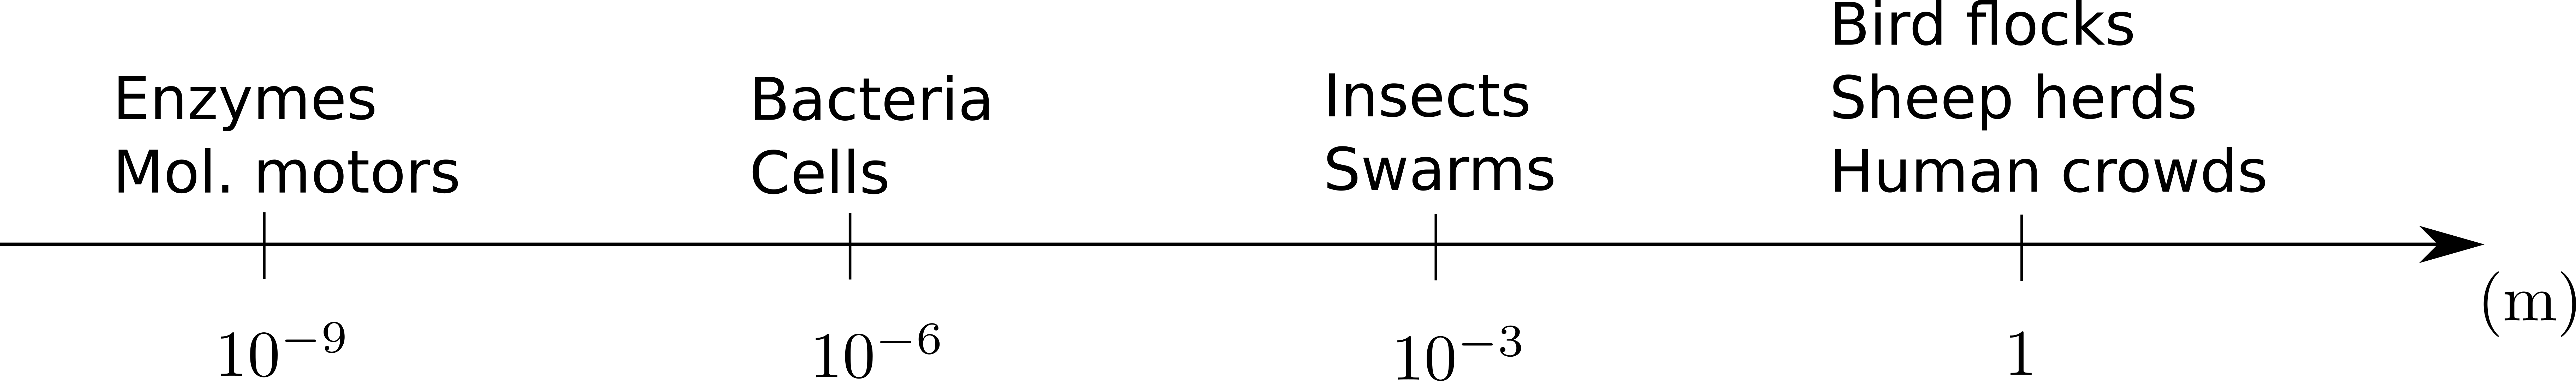
\includegraphics[width=.6\textwidth]{Figures/introduction/scales.png}
    \caption{The range of scales of active particles.}
    \label{fig: scales active particles}
\end{figure}


% Handwritten page II
Some examples of active systems are:

\begin{itemize}
    \item Enzymes and molecular motors, that evolve over the nanometer scale. Enzymes (E) catalyze chemical reactions of their substrate (S) into some product(s) (P),
    %s and cells. Bacteria and
    \begin{align}
        E + S \longrightarrow  \underbrace{SE}_{\mathrm{binding}} \longrightarrow  E + P,
    \end{align}
    %
     and thus locally sustains chemical gradients $\bm \nabla S$ and $\bm \nabla P$. 
     \begin{figure}[H]
        \centering
        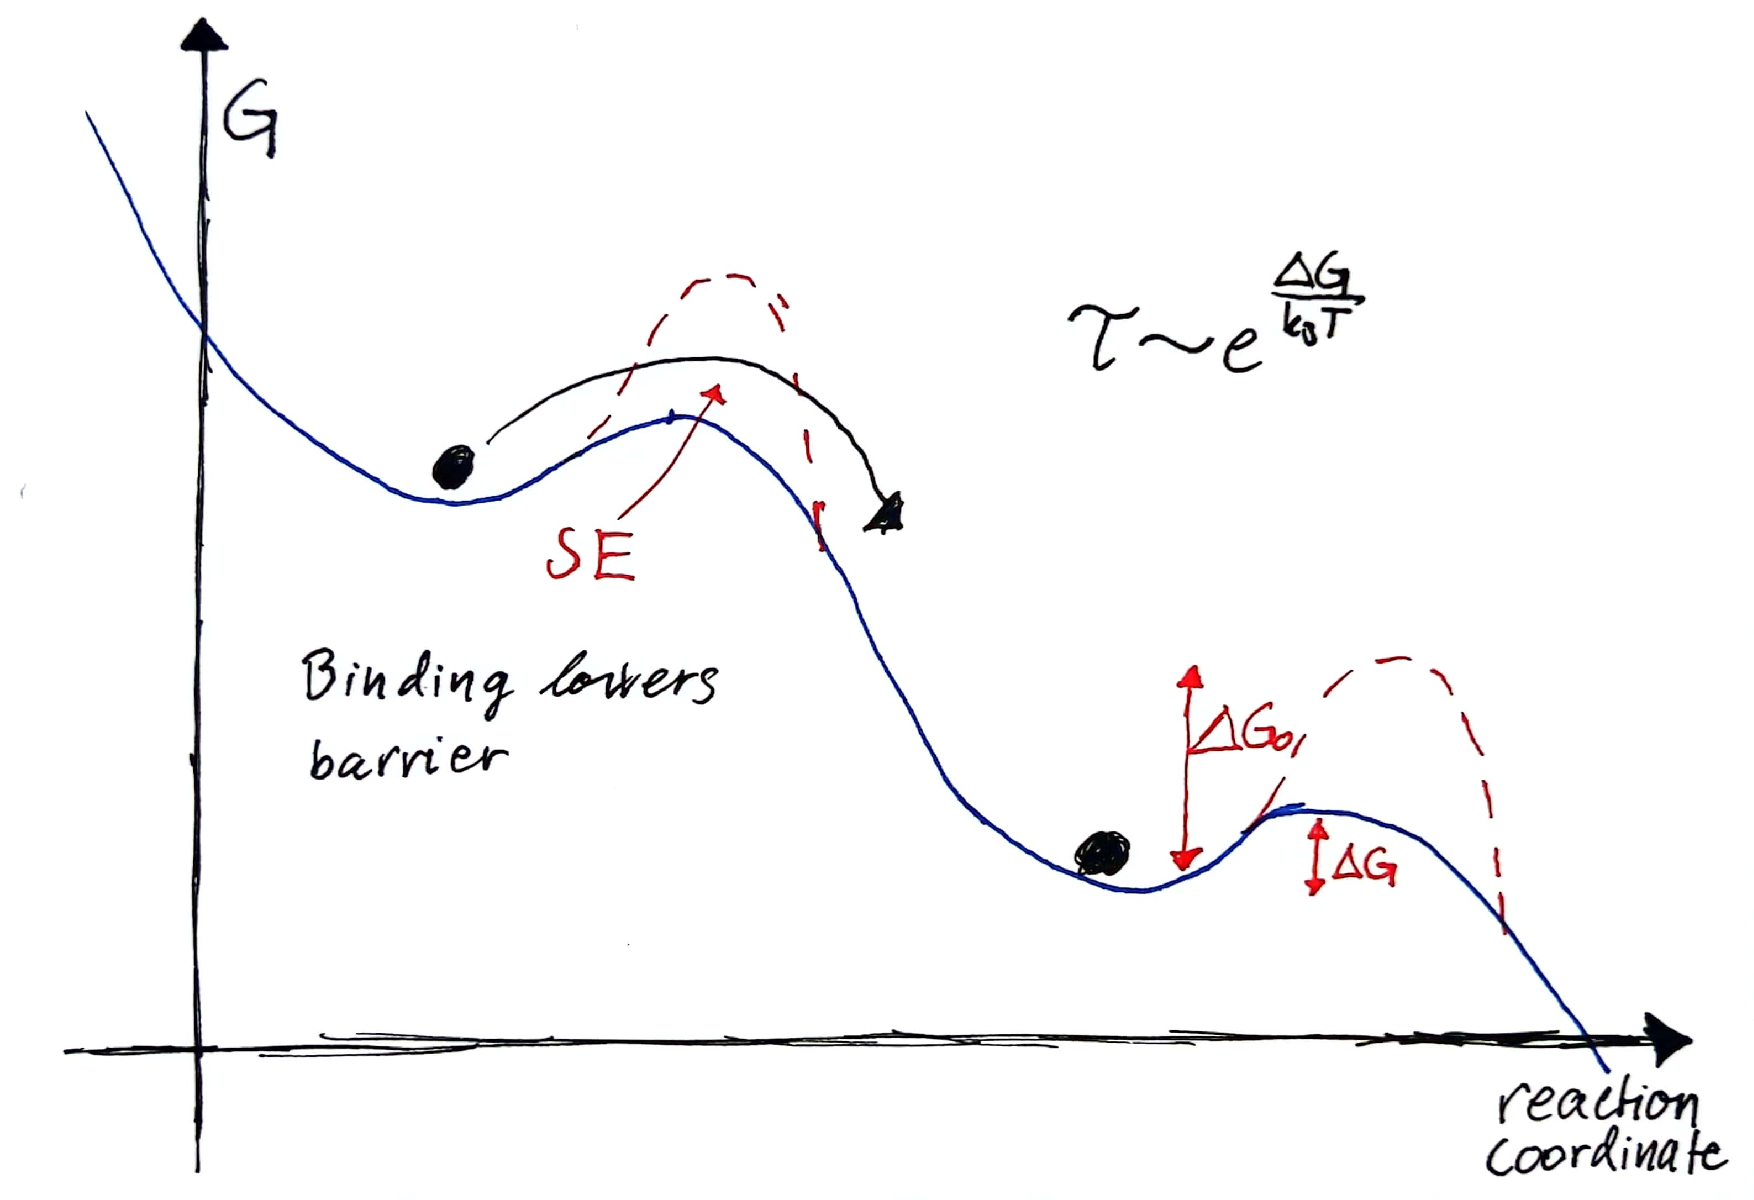
\includegraphics[width=.3\textwidth]{Figures/introduction/enzymes.pdf}
        \caption{A sketch of how an enzyme works. The enzyme lowers the effective free energy barrier associated with the $S \to P$ reaction. In the case where a constant supply of substrate is provided, the effect of the enzyme will therefore materialize in the production of chemical currents in some reaction coordinate space.}
        \label{fig: enzymes}
    \end{figure}
    %
    \item Molecular motors are a particular kind of enzyme for which chemical cycles are coupled to displacements or rotations so that these molecular machines can perform work and, e.g., self-propel.
     \begin{figure}[!h]
        \centering
        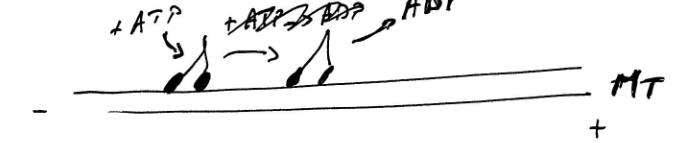
\includegraphics[width=.3\textwidth]{Figures/introduction/motors.png}
        \caption{Molecular motors consume ATP to travel along microtubules.}
        \label{fig: motors}
     \end{figure}
    \item Microorganisms and cells. Bacteria and algae usually move thanks to filamentous appendices called flagella or cilia, which are powered by molecular motors.
    Thanks to their internal machinery, these organisms are therefore able to displace the fluid around them, resulting in a self-propelled motion.
    Another example of self-propulsion at the micrometer scale can be found in some types of cells that are able to glide on substrates by performing cycles of polymerization and depolymerization of actin filaments.
    \begin{figure}[!h]
        \centering
        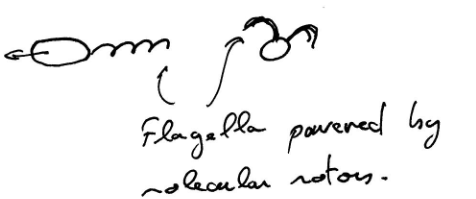
\includegraphics[width=.3\textwidth]{Figures/introduction/bacteria.png} 
        \hspace{2cm}
        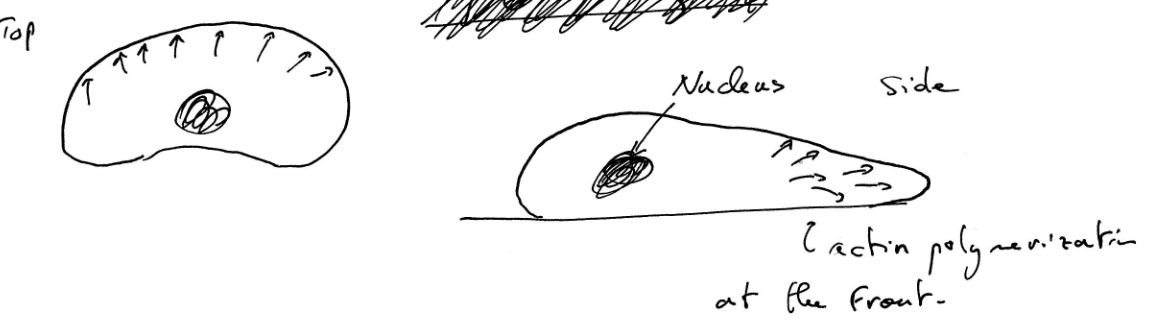
\includegraphics[width=.22\textwidth]{Figures/introduction/actin.png}
        \caption{Motion at a microscopic level: to the left, microswimmers move using flagella. 
        To the right, a cell moves by polymerizing actin filaments at its front.}
        \label{fig: label}
    \end{figure}
    %
    \item Many familiar examples of active entities are found at larger scales, this includes e.g. insect swarms at the millimeter scale, and animal herds or human crowds at (roughly) the meter scale.
\end{itemize}


% Handwritten page III

\subsection*{What makes active matter special?}

Active systems, because they constantly dissipate energy at the level of their elementary constituents, 
%and in contrast to passive systems globally driven (for example turbulent flows, shaken granulars, \ldots), 
are able to spontaneously self-assemble into complex and dynamic structures. 
Again, these ideas are relevant to many examples in the living world including the architecture of the cytoskeleton, the morphogenesis of multicellular organisms, or the collective motion arising from social interactions in groups of several hundred or thousands of individuals. 

Active matter is also not restricted to the study of biological systems, as the design and study of synthetic active particles now represent a large part of the field. Those allow for better controlled experiments and often exhibit similar phenomenology as their biological counterpart, thus opening the way to biomimetic materials engineering. 
Famous examples of artificial active matter include assemblies of self-propelled colloids (Phoretic Janus particles, so-called Quincke rollers), artificial microswimmers (self-propelled drops, magnetic swimmers), and robots~\cite{BechingerRMP2016}.

\begin{figure}[!htb]
    \centering
    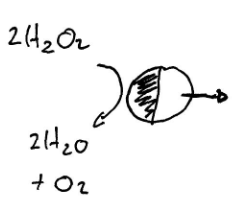
\includegraphics[width=.2\textwidth]{Figures/introduction/janus.png}
    \caption{A self-propelled Janus particle, to be discussed in Chapter~\ref{chap_phoretic}.}
    \label{fig: janus}
\end{figure}



\subsection*{On the nonequilibriumness of active assemblies}

As written above, active matter is inherently `far' from equilibrium, since it is assembled from particles whose dynamics constantly break time-reversal symmetry. This means that active systems lack most of the properties on which our intuition of systems at thermodynamic equilibrium is based. These include:
%
\begin{enumerate}
    \item \textit{Absence of minimization principle:} active dynamics are not constrained by the second law of thermodynamics so that they do not converge over long times to a state of maximal entropy (or minimum free energy). In fact, there is no general argument telling us whether the dynamics of a many-body active system converge to a steady state or not.
    \item \textit{No time-reversal symmetry (TRS):} as a consequence of the previous point, active systems can (and do) generally produce macroscopic currents, leading to phases where TRS is collectively broken.
    \item \textit{Lack of a thermodynamic framework:} Basic equilibrium concepts such as temperature or thermodynamic pressure are usually not defined for active systems. Additionally, active systems generally do not exhibit an equation of state, meaning that their bulk behavior is not only determined by their material properties but can also be substantially affected by the nature and shape of the container they live in. 
    \item \textit{The presence of memory:} again due to point 1, and contrary to systems at equilibrium, the state of an active system may be dependent on its history.
    \item \textit{Emergence of nonreciprocal couplings:} In active matter, momentum is not conserved so forces do not necessarily need to satisfy the action-reaction principle. Familiar examples of such `nonreciprocity' are encountered in predator-prey dynamics, while it also generally arises when particles interact via self-generated fields such as bacteria or phoretic colloids.
    The consequences of the presence of such couplings will be explored in chapter~\ref{chap_nrch}.
\end{enumerate}
%
In summary, the collective behaviors found in active systems generally break our intuition built on equilibrium physics, and their theoretical understanding requires the development of tools and concepts specifically tailored to address nonequilibrium dynamics.
In chapter~\ref{chap_thermo}, we will see how field theory descriptions of active systems can be obtained phenomenologically from the framework of irreversible thermodynamics, while coarse-graining techniques will be discussed in chapter~\ref{chap_scalar}.


% Handwritten Page IV

\subsection*{The idea of this course}

Active matter is very large and quickly developing field, borrowing tools and concepts from various other areas of physics including soft matter, biological physics, hydrodynamics, and statistical physics. Hence, this course is only meant as an introduction to the basics of the very diverse of active systems, and how it is usually apprehended. In particular, our journey will be driven by two general questions which are still the topic of ongoing research:
\begin{itemize}
    \item How is active motion generated at the micro scale, and what are its consequences on the dynamics of active particles?
    \item How do active systems convert energy dissipated at the molecular scale into the formation of structure and order macroscopic scales?
\end{itemize}
This first chapter is meant to give an overview of the topics that will be addressed in the following lectures, while we will also introduce physics concepts and mathematical tools that will be useful throughout these notes.

% Handwritten page V

\section{Hydrodynamics of microswimmers}
\label{sec: hydrodynamics of microswimmers}

Many (if not most) active particles evolve in a fluid, which they need to displace in order to move. Understanding the locomotion of such swimmers thus requires to study the dynamics of the flow around them. The fluid surrounding the particles is generally incompressible, so that it is defined by its local velocity $\bm v$ which obeys the Navier-Stokes (NS) equations:
%
\begin{subequations}
\label{eq_NS}
\begin{align}
    \label{eq_NS_v}
    \rho \left[ \partial_t \bm v + (\bm v \cdot \nabla)\bm v \right] & = \eta \nabla^2\bm v - \nabla P + \bm f, \\
    \label{eq_NS_inc}
    \nabla \cdot \bm v & = 0.
\end{align}
\end{subequations}
%
The terms on the left-hand side of~\eqref{eq_NS_v} correspond to the material derivative and simply model the effect of inertia, while on the right-hand side the first term originates from viscous dissipation, the second is the pressure which ensures incompressibility as required by~\eqref{eq_NS_inc}, while the active force $\bm f$ arises as a source term.
In cases dominated by inertia or dissipation, the NS Eq.~\eqref{eq_NS} simplifies. To understand this, let us define the typical length and velocity scales of the problem, $L$ and $V$, and apply the following rescalings:
%
\begin{equation*}
    \bm v \to V \bm v', \quad
    \bm x \to L \bm x', \quad
    t \to \frac{L}{V}t', \quad
    P \to \frac{\eta V}{L} P', \quad
    \bm f \to \frac{\eta V}{L^2} \bm f'.
\end{equation*}
%
We then obtain the following equation in terms of the dimensionless primed variables
%
\begin{equation}
    {\rm Re}\left[ \partial_{t'} \bm v' + (\bm v' \cdot \nabla')\bm v' \right] = \nabla'^2\bm v' - \nabla' P' + \bm f',
\end{equation}
%
where the dimensionless quantity ${\rm Re} = \rho V L / \eta$ is known as the Reynolds number. 
Alternatively, note that the Reynolds number can be obtained by taking the ratio of the typical scales associated with the convection $\rho(\bm v\cdot \nabla )\bm v$ and dissipation $\eta\nabla^2\bm v$ terms in~\eqref{eq_NS}. 
Hence, the value of the Reynolds number controls the relative importance of inertial effects and viscous dissipation.
For a micron-sized swimmer in water such as bacteria, we can evaluate $\rho \approx 10^3 \; {\rm kg / m^3}$, $\eta \approx 10^{-3} \; {\rm Pa \cdot s}$,
$V \approx 10^{-5}\; {\rm m/s}$, and $L \approx 10^{-6} \; {\rm m}$, such that ${\rm Re} \approx 10^{-5}$.
%
% Handwritten page VI
%
\textit{Microswimmers, therefore, live in a world at basically zero Reynolds number} where inertial effects are negligible. 
Their dynamics then evolve in the so-called Stokes regime, 
such that the flow they generate obeys the Stokes equation:
%
\begin{subequations}
\label{eq_Stokes}
\begin{align}
    \label{eq_Stokes_v}
    \eta \nabla^2\bm v -\nabla P + \bm f & = \bm 0, \\
    \label{eq_Stokes_inc}
    \nabla \cdot \bm v & = 0.
\end{align}
\end{subequations}
%
Contrary to the Navier-Stokes equation, Eqs.~\eqref{eq_Stokes_v} do not have time derivatives and is linear.
The flow velocity $\bm v$ thus only depends on the instantaneous value of the force $\bm f$ (there is no inertia), and it varies linearly with it\footnote{By taking the divergence of~\eqref{eq_Stokes_v}, you can convince yourself that the pressure is also a linear function of the force.}. 
An important consequence of these features is that is that Stokes flows obey kinematic reversibility, meaning that they satisfy the symmetry
%
\begin{equation*}
    \bm f \rightarrow -\bm f, \qquad \bm v \rightarrow -\bm v.
\end{equation*}
%
As such, sequences of motion are reversible.
One important consequence of this is the \emph{scallop theorem}, which states that a microswimmer cannot achieve self-propulsion with reciprocal motion.
%
\begin{figure}[!htb]
    \centering
    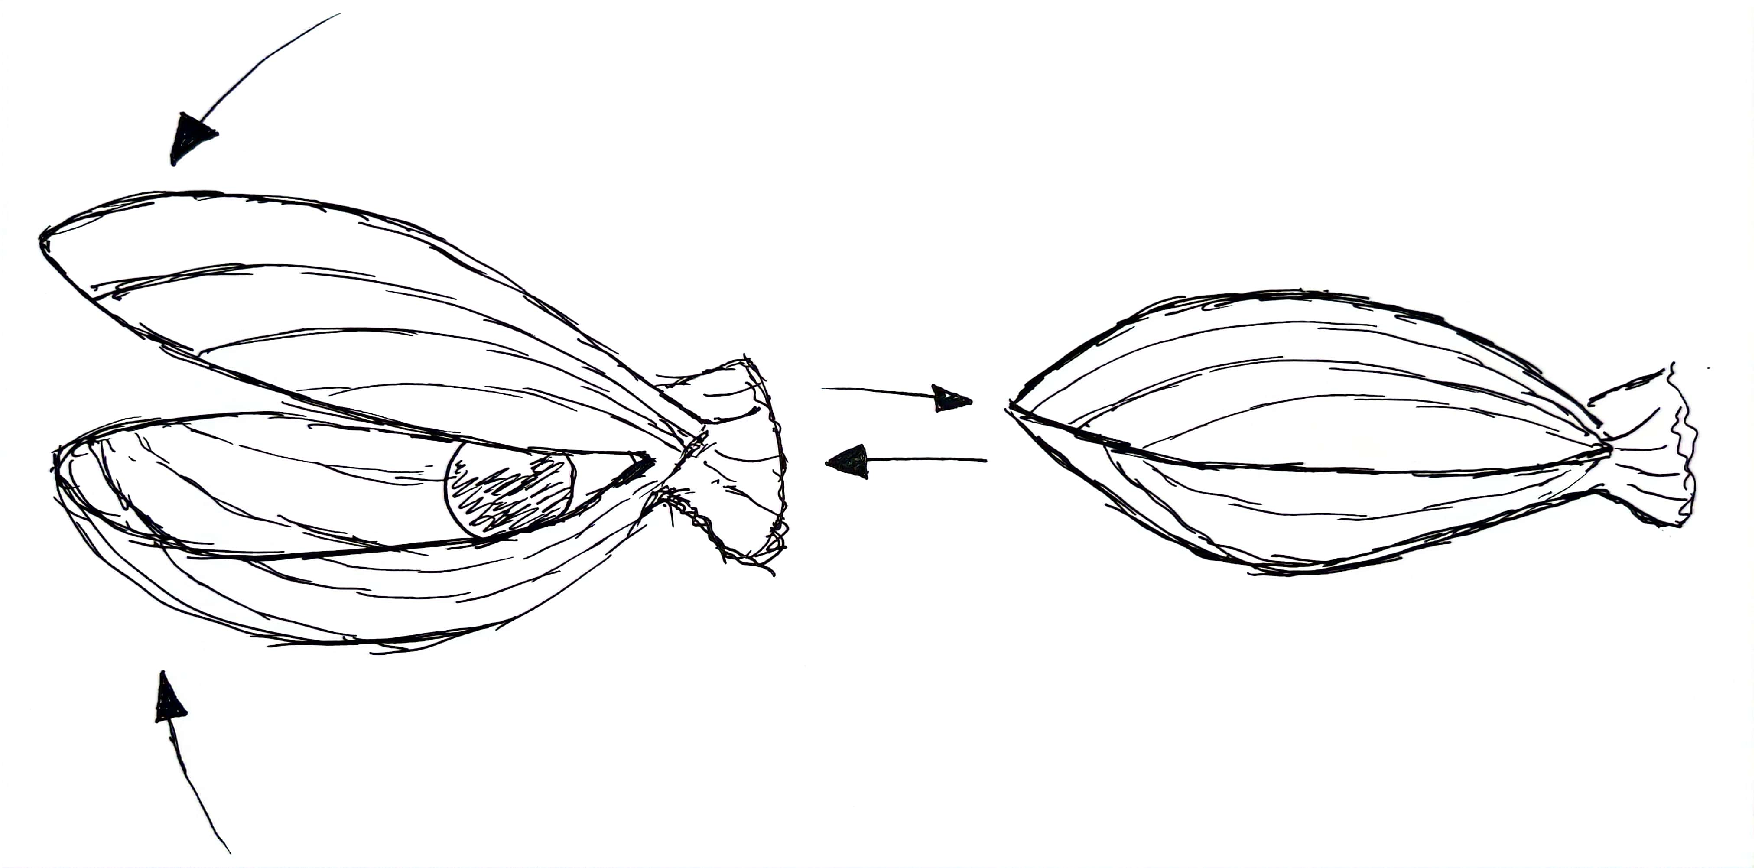
\includegraphics[width=.5\textwidth]{Figures/introduction/scallop.pdf}
    \caption{A scallop moves by opening and closing its shells, which in the Stokes regime gives zero net motion}
    \label{fig: scallop}
\end{figure}

The name comes from an example of reciprocal motion, a scallop opening and closing its shell.
A nonzero net self-propulsion therefore requires for the active particle to perform nonreciprocal cycles in configuration space.
The solutions nature has found to overcome this problem include rotating a bundle of helical flagella, as is done by \textit{E. coli}, or using additional degrees of freedom allowing, e.g., to perform breast-stroke-like motion, as is done by \textit{Chlamydomonas}.

\begin{figure}[!htb]
    \centering
    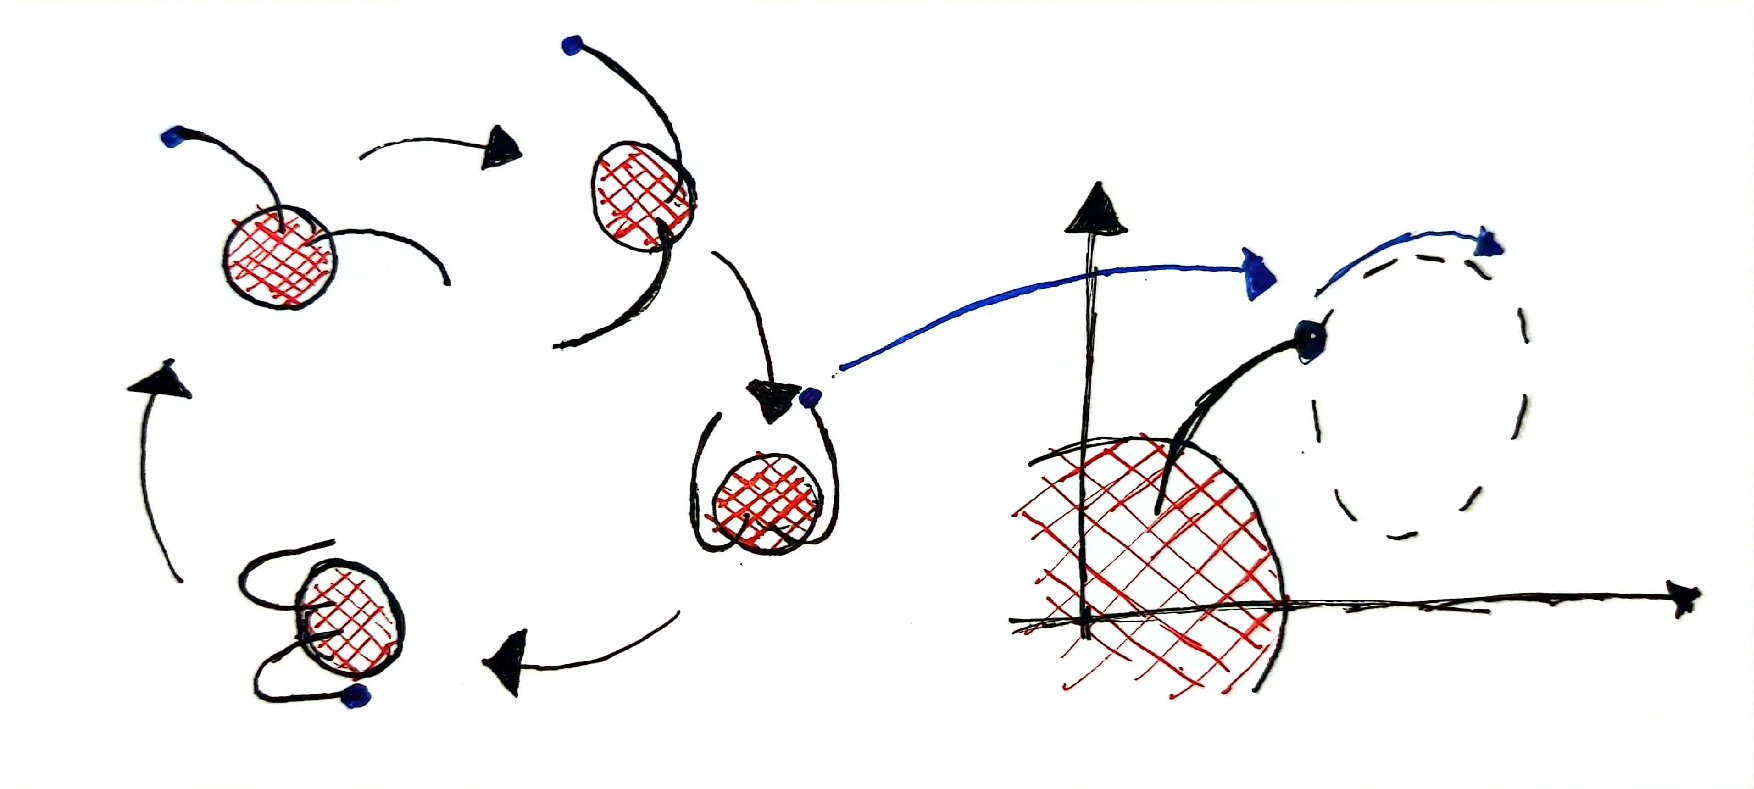
\includegraphics[width=.4\textwidth]{Figures/introduction/breast_stroke.pdf}
    \caption{
        A schematics illustrating how the breaststroke of a flexible flagellum follows a nonreciprocal cycle in configuration space.
        If the stroke consisted instead of a back-and-forth motion of a rigid flagellum --as is the case with the scallop-- any of its point would trace a line enclosing no area.
    %By following the tip of the flagellum.
    %If the stroke was the same backwards and forwards, the tip would trace out a line instead of a circle, and thus enclose no area in configuration space.
    %This is the case when following any point on the scallop, and is why it would achieve no net motion in the Stokes regime. 
    }
    \label{fig: breast stroke}
\end{figure}


Another consequence of the absence of inertia in the Stokes regime is that the swimmers cannot experience any net force or torque (the Stokes equation corresponds to a balance of momentum).
A net force would lead to acceleration, which by assumption is zero in the Stokes regime.
Hence, the force and torque generated by the flagella of the swimmers shown in Fig.~\ref{fig: swimmers} must be compensated by the drag their body exerts on the fluid\footnote{Assuming that the drag coming from the flagella is negligible.}. 
In the far field, most microswimmers can thus be modeled as force and/or torque dipoles.
Analogously to electric dipoles, force dipoles exert no net force on the fluid, but still generate a nonzero flow field.
%Force dipoles are similar to electric dipoles, points with zero charge but which still affect the electric field, as they are points where the net force is zero but which still affect the flow field.
The nature of the dipole 
depends on how the swimmer locally actuates the fluid.
For example, swimmers propelling by pushing the fluid at their rear like \textit{E. coli} are named `pushers', while those pulling the fluid in front of them like \textit{Chlamydomonas} are named `pullers'. 

\begin{figure}[!htb]
    \centering
    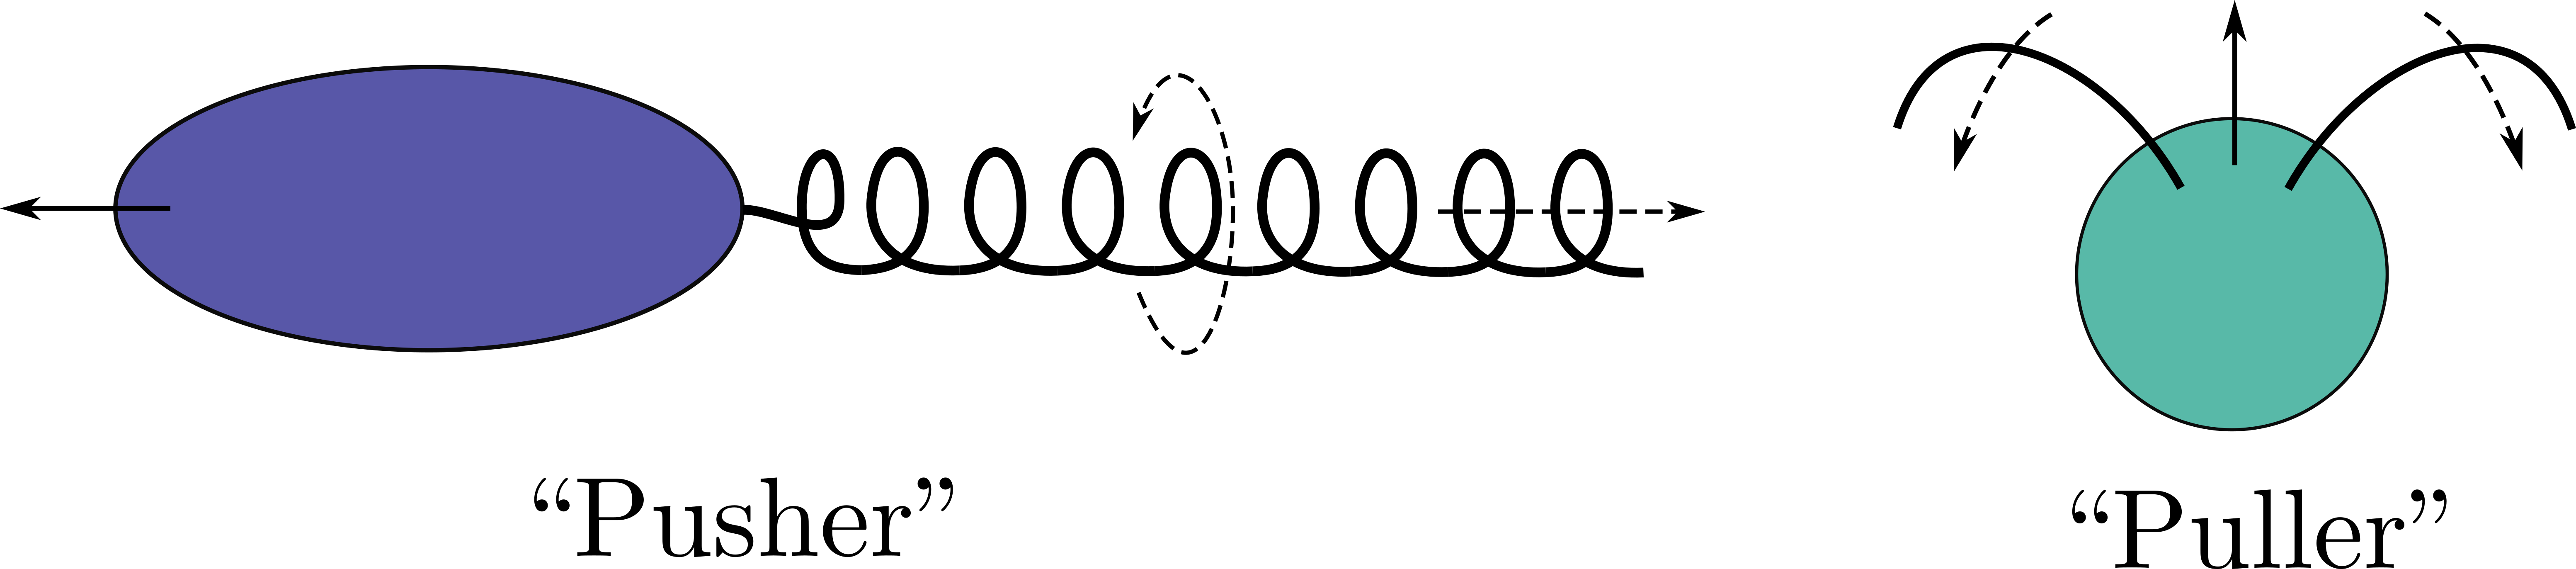
\includegraphics[width=.5\textwidth]{Figures/introduction/swimmers.png}
    \caption{Two examples of microswimmers showing the so-called \textit{pusher} and \textit{puller} configurations,
    corresponding to dipoles with forces pointing outwards and inwards, respectively.
    In both cases, the forces exerted by the flagella on the fluid are compensated by the drag. 
    }
    \label{fig: swimmers}
\end{figure}

We have seen that, because of the constraints imposed by Stokes flows, generating active motion at microscopic scales is far from being a simple task. The design and characterization of microscimmer self-propulsion mechanisms is in fact an active area of research. 
In Chapter~\ref{chap_hydro}, we will discuss microswimmers hydrodynamics in more details.

% handwritten page VII

\section{A minimal model for active motion}
\label{intro_ABM}

In the previous section, we have discussed by which mechanism(s) active motion can arise in the context of microswimmers.
Here, we will ask a different question: what are the consequences of the presence of a self-propulsion speed on the dynamics of an active particle?
For this, we will model our swimmer/crawler/glider as an abstract `particle', and assume that it is able to sustain a finite self-propulsion velocity, but we won't be interested in the details of how this self-propulsion is realized.


\subsection*{Some basics on Brownian motion}

\begin{figure}[!htb]
    \centering
    \includegraphics[width=.4\textwidth]{Figures/introduction/brownian.png}
    \caption{A Brownian particle is constantly interacting with the solvent molecules, resulting in an erratic motion.}
    \label{fig: brownian}
\end{figure}

Before discussing active motion, let us give a brief recap on the theory of the motion of Brownian (i.e. dead) particles.
Consider a micron-sized particle (e.g. a grain of pollen, a colloid, etc..) in a fluid maintained at temperature $T$. 
The particle constantly undergoes collisions with the fluid molecules, and its mass is low enough so that these collisions result in an apparent erratic dynamics known as Brownian motion.
The dynamics of the particle can be modeled by the \emph{Langevin equation}
%
\begin{equation} \label{eq_LangevinBM}
    m\frac{\rmd^2 \bm r}{\rmd t^2} + \zeta \frac{\rmd \bm r}{\rmd t} = \bm f(t).
\end{equation}
%
Equation~\eqref{eq_LangevinBM} is nothing but Newton's second law, so that the first term on the left hand side represents the acceleration of the particle multiplied by its mass, and the second term accounts for the Stokes friction exerted by the fluid in response to the motion of the particle.
In fact, the ratio of the particle mass and friction coefficient defines a timescale $\tau = m / \zeta$ beyond which inertial effects can be neglected.
For a micron-sized sphere with a density comparable to that of water, we have
%
\begin{equation*}
    \tau = \frac{\rho \tfrac{4\pi}{3} R^3}{6 \pi \eta R} 
    = \frac{2\rho R^2}{9\eta} \approx 0.2 \; \mu{\rm s}.
\end{equation*}
%
For observation times beyond the micro-second, inertial effects can therefore be safely neglected. Hence, we will neglect the inertial term in~\eqref{eq_LangevinBM}, which we re-express in this overdamped limit as
\begin{equation} \label{eq_LangevinBM_ovd}
    \frac{\rmd \bm r}{\rmd t} = \frac{1}{\zeta}\bm f(t).
\end{equation}
%
The force term $\bm f$ is meant to model the random collisions that the particle undergoes with the solvent molecules, and is thus stochastic in nature.
Under the approximation that these collisions are isotropic, identically distributed and uncorrelated random events, we can use the central limit theorem to approximate the distribution of the stochastic process $\bm f$ by a normal distribution with zero mean and variance $\sigma^2$.
Namely, denoting averages with independent realizations of the noise with the notation $\langle \cdot \rangle$, the first two moments that fully characterize the distribution read
\begin{equation*}
    \langle f_i(t) \rangle = 0, \qquad
    \langle f_i(t) f_j(t') \rangle = \sigma^2 \delta_{ij}\delta(t - t').
\end{equation*}

Equation~\eqref{eq_LangevinBM_ovd} can be easily solved by integration, which leads to
\begin{equation*}
    \Delta \bm r(t) \equiv \bm r(t) - \bm r(t=0) = \frac{1}{\zeta} \int_0^t\rmd\tau \bm f(\tau).
\end{equation*}
Taking averages over the noise, this solution implies in particular that 
\begin{equation} \label{eq_BM_moments}
    \langle \Delta \bm r(t) \rangle = \bm 0, \qquad 
    \langle |\Delta \bm r(t)|^2 \rangle = d \sigma^2 t / \zeta^2,
\end{equation}
where $d$ is the number of spatial dimensions.
Equation~\eqref{eq_BM_moments} summarizes the two main features of Brownian (or diffusive) motion: it is associated with no net motion and leads to a mean-squared displacement (MSD) linear in time.
The quantity $D = \sigma^2 / 2 \zeta^2$ is the diffusion coefficient of the particle.
Since both the viscous drag and stochastic force in~\eqref{eq_LangevinBM_ovd} originate from interactions between the particle and the solvent, the diffusion and friction coefficients are related by Einstein relation as $D = k_{\rm B}T / \zeta$.
This relation belongs to a more general class of equalities known as fluctuation-dissipation relations, and which are a hallmark of equilibrium (or near-equilibrium) dynamics.

\noindent
\textbf{Homework:} \textit{ By solving~\eqref{eq_LangevinBM} for the particle velocity $\bm v = \dd\bm r / \dd t$, show that the equipartition theorem imposes $\sigma^2 = 2 \zeta k_B T$. Deduce Einstein's relation from this result.
}

% Hand written page VIII

The problem of overdamped Brownian motion is sufficiently simple so that one can determine the full statistics of the particle displacement. 
For this, we define $\calP(\bm x,t) = \langle \delta(\bm x - \bm r(t)) \rangle$ as the distribution of the particle position, which obeys the Fokker-Planck equation
%
\begin{equation} \label{eq_FP_BM}
    \partial_t \calP(\bm x,t) - D \nabla^2 \calP(\bm x,t) = 0.
\end{equation}
%
Assuming that the particle sits at $\bm x = \bm 0$ at time $t=0$, the solution of Equation~\eqref{eq_FP_BM} is given by
\begin{equation*}
    \calP(\bm x,t) = \frac{1}{(4\pi D t)^{d/2}}e^{-\tfrac{|\bm x|^2}{4 D t}}.
\end{equation*}
We note that the mean of the distribution is at $\bm x = \bm 0$ at all times and that its width, i.e. the standard deviation, grows as $\sqrt{t}$ consistently with~\eqref{eq_BM_moments}.


\textit{
{\bf Homework:}
It\^o's lemma corresponds to the chain rule of stochastic calculus. Given a stochastic process $\bm x(t)$ satisfying the Langevin equation $\tfrac{\dd\bm x}{\dd t} = \bm a + b \bm \xi(t)$,
it states that any twice differentiable function $f(\bm x,t)$ satisfies
\begin{equation*}
    \frac{\dd f}{\dd t} = \frac{\partial f}{\partial t} + \bm a\cdot\nabla f + \frac{b^2}{2}\nabla^2 f + b (\nabla f)\cdot \bm \xi(t).
\end{equation*}
\begin{enumerate}
    \item Considering an arbitrary function $f(\bm x)$, we define its average as $\E{f} = \int \dd\bm x \, f(\bm x) \calP(\bm x,t)$.
    Express $\E{\tfrac{\dd f}{\dd t}}$ as a function of $\partial_t \cal P$ and, using It\^o's lemma, also show that
    \begin{equation*}
        \E{\frac{\dd f}{\dd t}} = 
        \E{\bm a \cdot \nabla f} + \E{\frac{b^2}{2}\nabla^2 f}
        = \int\dd\bm x\, f(\bm x) \left[-\nabla \cdot(\bm a \calP) 
        + \frac{1}{2}\nabla^2\left(b^2\calP \right)\right].
    \end{equation*}
    Using that $f$ is arbitrary, deduce the Fokker-Planck equation satisfied by $\calP(\bm x,t)$.
    \item Consider a Brownian particle in a potential $U$, write the associated Fokker-Planck equation. Show that the stationary solution corresponds to the Boltzmann distribution.
    For a harmonic potential $U = \tfrac{1}{2} k |\bm x|^2$, the time dependent solution of the FPE with initial condition $\calP(\bm x,0) = \delta(\bm x)$ is given by 
    \begin{equation*}
    \calP(\bm x,t) = \left(\frac{\lambda}{2\pi D (1 - e^{-2\lambda t})}\right)^{d/2}e^{-\tfrac{\lambda}{2 D} \tfrac{|\bm x|^2}{1 - e^{-2\lambda t}}},
    \end{equation*}
    with $\lambda = k / \zeta$.
    Calculate the mean and MSD associated with this distribution, comment.
\end{enumerate}
}

\subsection*{Active Brownian motion}

Although the previous section was devoted to the description of the dynamics of a passive particle, the Langevin equation~\eqref{eq_LangevinBM_ovd} does not assume that the particle is in an equilibrium state. 
Therefore, we can straightforwardly generalize to describe active motion it by assuming that the particle is able to self-generate a force leading to an active velocity $\va(t)$.  Equation~\eqref{eq_LangevinBM_ovd} now becomes
\begin{equation}\label{eq_LangevinABM}
    \frac{\rmd \bm r}{\rmd t} = \va(t) + \frac{1}{\zeta}\bm f(t).
\end{equation}
To fully characterize the dynamics, we now need to specify how $\va(t)$ evolves in time. 
As we have seen previously, self-propelled motion can arise in various ways, but what we argue below is that it most importantly introduces a finite persistence length in the dynamics.

To understand this, let us comment on real systems.
For example, the dynamics of bacteria like \textit{E. coli} consists of randomly alternating sequences of `run' and `tumble', respectively corresponding to straight motion along a fixed direction and random reorientations. 
Other active swimmers like self-propelled colloids, on the other hand, follow smooth trajectories as their self-propulsion direction slowly diffuses over time due to fluctuations.
In both cases, defining the typical particle velocity as $v_0$ and reorientation time $\tau_r$, we can build a persistence length by dimensional analysis as $\lp = v_0 \tau_r$.
Physically, on length scales below $\lp$ the active particle exhibits ballistic motion along a fixed direction with a speed $\approx v_0$, while on scales $\gg \lp$ its direction of motion has randomized so that its overall dynamics is isotropic and diffusive. 


\begin{figure}[!htb]
    \centering
    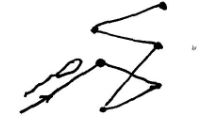
\includegraphics[width=.25\textwidth]{Figures/introduction/runandtumble.png}
    \hspace{2cm}
    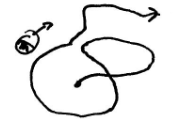
\includegraphics[width=.2\textwidth]{Figures/introduction/smooth.png}
    \caption{Run-and-tumble versus smooth active trajectories resulting from different modes of self-propulsion.}
    \label{fig: run and tumble vs smooth}
\end{figure}

As a minimal model of active velocity, we can thus simply assume that the particle self-propels at constant speed $v_0$, while the unit vector $\he$ parametrizing its orientation is a colored noise with zero mean and exponential correlations:
\begin{equation} \label{eq_cf_e}
    \langle \he(t) \cdot \he(t + \tau) \rangle = e^{-\tau / \tau_r}.
\end{equation}

\textit{
\noindent 
    {\bf Homework:} 
    Consider an active particle moving in two dimensions,
    so that its self-propulsion direction is parametrized by a single angle $\theta(t)$.
    \begin{enumerate}
        \item Modeling tumbles as isotropic and uncorrelated random events occurring with a rate $\lambda$, show that the associated probability distribution is given by
        \begin{equation*}
            P(\theta,t) = e^{-\lambda t}\delta(\theta) + \frac{1}{2\pi}\left(1 - e^{-\lambda t} \right).
        \end{equation*}
        Here, we have assumed for simplicity that $\theta = 0$ at time $t = 0$.
        \item In the case where $\theta$ diffuses in time with a diffusion coefficient $D_r$, show that the associated distribution is a Gaussian with zero mean and variance $2 D_r t$.
        \item For both cases 1. and 2. deduce that the 
        particle self-propulsion direction satisfies $\E{\hat{\bm e}(\theta(0))\cdot \hat{\bm e}(\theta(\tau))} = \exp(-\tau/\tau_r)$, and express $\tau_r$ as a function of $\lambda$ and $D_r$.
    \end{enumerate}
    }


We immediately deduce from~\eqref{eq_cf_e} that, under the assumption that the active and Brownian noises are independent,
\begin{align}
    \langle |\Delta \bm r(t)|^2 \rangle & = 2 d D t 
    + v_0^2 \int_0^t\rmd\tau_1\int_0^t\rmd\tau_2 \, e^{-|\tau_1-\tau_2|/\tau_r} \nonumber \\
    & = 2 d D t 
    + 2 \lp^2 \left( \frac{t}{\tau_r} - 1 + e^{-t/\tau_r} \right).
\end{align}
%
This expression can be simplified by considering the limiting regimes $t \gg \tau_r$ and $t \ll \tau_r$,
which respectively give
%
\begin{align*}
    \langle |\Delta \bm r(t)|^2 \rangle & 
    \underset{t \ll \tau_r}{\simeq} 2 d D t + v_0^2 t^2 , \\
    \langle |\Delta \bm r(t)|^2 \rangle & 
    \underset{t \gg \tau_r}{\simeq} 2 d D_{\rm eff} t , \qquad  D_{\rm eff} = D + \frac{v_0^2\tau_r}{d}. 
\end{align*}
%
The active particle MSD therefore highlight three dynamical regimes shown in Fig.~\ref{fig: MSD}:
\begin{itemize}
    \item Thermal diffusion dominates at short times ($t \ll 2 d D / v_0^2)$.
    \item At intermediate times ($2 d D / v_0^2 \ll t \ll \tau_r)$, activity contributes and motion is ballistic with a typical speed $v_0$.
    \item At long times ($t \gg \tau_r$) the self-propulsion direction has randomized, resulting in a diffusive motion with an enhanced diffusion coefficient.
\end{itemize} 

Due to the finite correlation time of its self-propulsion orientation, the long-time dynamics of an active particle is therefore ``Brownian-like'' (i.e. diffusive).
However, the associated effective diffusion coefficient $D_{\rm eff}$ does not satisfy the fluctuation-dissipation relation, which is a clear signature that the dynamics is out-of-equilibrium.

\begin{figure}[!htb]
    \centering
    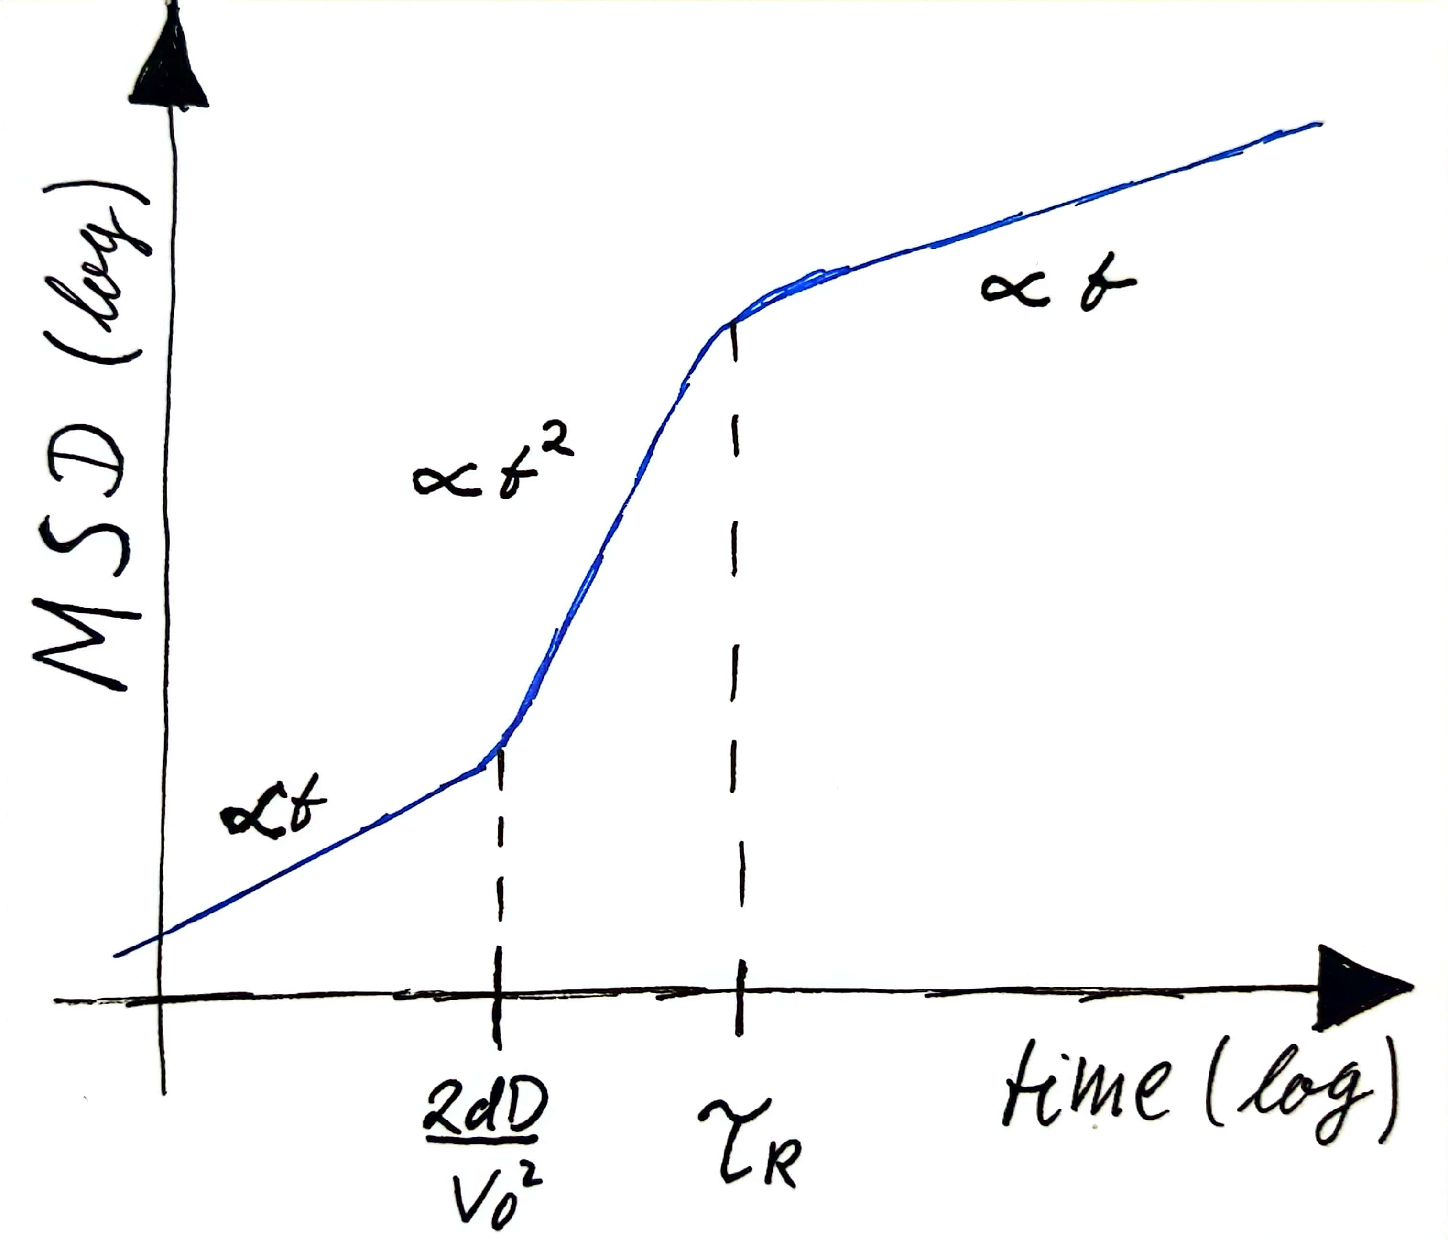
\includegraphics[width=.4\textwidth]{Figures/introduction/crossover.pdf}
    \caption{The mean-square displacement of an active Brownian particle showing the three dynamical regimes discussed in the main text.}
    \label{fig: MSD}
\end{figure}



% Handwritten page XIII

\section{Phase transitions and critical phenomena}

The concept of phase transition plays a central role in the study of active systems.
A prominent example the emergence of flocking behavior which we will study in more details in Chapter~\ref{chap_polar}, where directed units spontaneously choose a direction to align in and move together as a flock.
This phenomenon can be conceptually interpreted as a nonequilibrium phase transition, where rotational symmetry is spontaneously broken.
In some sense, flocks thus correspond to an active version of ferromagnetic materials, where spins do not sit on the sites of a lattice but can freely move.
%This is the Active Matter version of the ordering transition in the Ising model, in which spins align in the case of a ferromagnet or anti-align in the case of an anti-ferromagnet.
In this section, we will review some of the basic features of the theories of phase transitions at equilibrium, and introduce tools that will be useful in the context of active matter.



\subsection*{A simple example: the Ising model}

One of these important features of phase transitions is that they are associated with the notion of scale-invariance.
The simplest illustration of this can be obtained by analyzing the Ising model.
We consider $N$ spins, $s_i = \pm 1$ on a lattice, and define an energy function as
%
\begin{align} \label{eq_energy_Ising}
    E = - \frac{J}{2} \sum_{\E{ij}} s_i s_j.
\end{align}
%  
Here, $\E{ij}$ indicates that the sum is over all pairs of neighbors $(i,j)$ on the lattice, while the factor $\tfrac{1}{2}$ prevents double counting. 
For $J > 0$, minimizing $E$ will thus favour configurations for which neighbouring spins are aligned, while if $J < 0$ they will preferably anti-align.
The equilibrium state of the model is captured by the partition function, which in the canonical ensemble is obtained by summing the Boltzmann weights associated with all possible spin configurations $\{s_i\}$:
%
\begin{align}
    Z = \sum_{\{s_i\}} e^{-\beta E},
\end{align}
%
where $\beta = (k_B T)^{-1}$.
To measure the amount of order in the system, we also define the order parameter,
%
\begin{align}
    m = \frac{1}{N}\sum_i s_i,
\end{align}
%
which is usually called the magnetization.
If all spins points along the same direction $|m|  = 1$, while if they completely disordered $m \to 0$.

To get a qualitative understanding of the phenomenology of the model, we use a simple mean-field analysis and assume that each spin weakly fluctuates around its mean value $m$, so that we write $s_i \approx m + \delta s_i$, with $\delta s_i$ small.
Then, at linear order in the perturbation,
%
\begin{align*}
    s_i  s_j = m^2 + m(\delta s_i + \delta s_j) + \Oh(\delta s^2)
    \approx m(s_i + s_j - m).
\end{align*}
%
%Here, we have neglected terms that are second order in the perturbations $\delta s$.
% Handwritten page XIV
Under this assumption, we rewrite the total energy~\eqref{eq_energy_Ising} as
%
\begin{align*}
    E_{\rm MF} 
    &= \frac{1}{2} J m \sum_{\E{ij}}(m - s_i - s_j)
    = \frac{1}{2} J m z \left(m N - 2 \sum_{i} s_i  \right).
\end{align*}
%
Here, $z$ is the number of nearest neighbors for each site, i.e. the coordination number of the lattice.
Its value depends on the structure of the lattice and the dimensionality of space.
For square and cubic lattices, $z = 2 d$, where $d$ is the dimension of space.
At the mean field level, the partition function therefore reads
%
\begin{align}
    Z_{\rm MF} & = \sum_{\{s_i\}} \exp \left\{\frac{1}{2}\beta J m z \left( 2\sum_{i} s_i - mN \right) \right\} \nonumber \\
    & = e^{-\frac{1}{2}\beta J z N m^2} 
    \sum_{\{s_i\}} \prod_{i} e^{\beta J m z s_i} \nonumber \\
    & = e^{-\frac{1}{2}\beta J z N m^2} 
    \left[\sum_{s = \pm 1} \exp \left(\beta J m z s \right)\right]^N \nonumber\\
    & = e^{-\frac{1}{2}\beta J z N m^2} \left[2 \cosh \beta J m z\right]^N. \nonumber
\end{align}
%
The Helmholtz free energy of the system is obtained by taking the logarithm of the partition function, $\beta F = - \ln Z$, so that
%
\begin{align} \label{eq_Ising_FMF}
    \beta F_{\rm MF} = N \left[ \frac{1}{2}\beta Jm^2 z - \ln\left(\cosh \beta J m z\right) \right],
\end{align}
%
where we have discarded irrelevant constant contributions.
At constant volume and temperature,  the equilibrium state of the system minimizes the total free energy.
The magnetization of the system is therefore obtained from 
%
\begin{align} \label{eq_Ising_mMF}
    \pdv{F_{
    \rm MF}}{m} = 0
    \iff m = \tanh (\beta J m z).
\end{align}
%

\begin{figure}[!b]
    \centering
    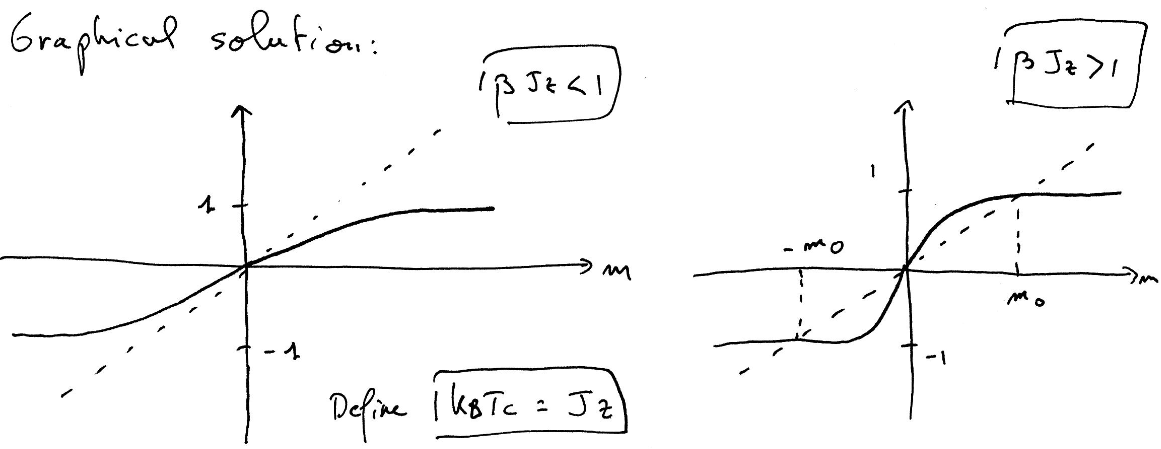
\includegraphics[width=.6\textwidth]{chapters/Figures/introduction/minimize.png}
    \caption{Graphical solution for the mean field magnetization.}
    \label{fig: The graphical solution of the mean field free energy minimization.}
\end{figure}

Equation~\eqref{eq_Ising_mMF} can be solved graphically by drawing both its l.h.s.\ and r.h.s.\ as a function of $m$, as illustrated in Fig.~\ref{fig: The graphical solution of the mean field free energy minimization.}.
In particular, we note that the $\tanh(\beta J m z)$ function is strictly monotonous in $[-1;1]$, while its maximum slope at $m=0$ is given by $\beta J z$. 
Therefore, when $\beta J z < 1$ the only solution of~\eqref{eq_Ising_mMF} corresponds to $m = 0$,
while for $\beta J z > 1$ a pair of additional solutions $m = \pm m_0 \ne 0$ emerges.
Taking the second derivative of $F_{\rm MF}$, one can also show that for $\beta J z > 1$ the solutions $m = \pm m_0$ correspond to two degenerate minima, while $m = 0$ is a local maximum.

Hence, there exists is finite value of the system temperature $k_B T_c = J z$ that marks a qualitative change in the equilibrium properties of the system.
This is exactly the definition of a phase transition, which is here associated to the emergence of a macroscopic magnetization in the system. 
% This shows that for inverse temperatures $\beta = 1 / k_B T$ so that $\beta J z < 1$, there is only one stationary point free energy, $m = 0$.
% In this case, this is also a minimum.
% For $\beta J z > 1$, there appear two additional stationary $m = \pm m_0$ points.
%These are now two degenerate minima of the free energy, while $m = 0$ is a local maximum.
%There is thus a \emph{phase transition} at the finite, critical temperature defined by $k_B T_c = J z$.
For $T \le T_c$, the $m \rightarrow - m$ symmetry of the theory is spontaneously broken, as the magnetization $m$ randomly settles at one of the degenerate minima $\pm m_0$.
If we now study the behavior of the system close to the transition, we can assume that $m$ is small and expand the free energy around $T \approx T_c$
so as to obtain a simplified expression known as the \textit{Landau free energy}:
%
\begin{align} \label{eq_LandauFE_Ising}
    F_{\rm MF}
    \underset{T \to T_c}{\simeq} 
    \frac{1}{2} Nk_B T_c
    \left( \vartheta m^2 + \frac{m^4}{6}\right)
    + \Oh(m^6),
\end{align}
%
where we have defined the reduced temperature $\vartheta \equiv (T - T_c) / T_c$, often called the control parameter. 

Thanks to its simple form, it is easier to get an intuitive picture from~\eqref{eq_LandauFE_Ising} of the changes in the free energy landscape that induce the phase transition.
%t has the form $F = \frac{1}{2} \alpha t m^2 + \beta \frac{1}{4} m^4$.
As $\vartheta$ changes sign, the free energy transitions from a single-well to a double-well structure with two degenerate minima.
This feature is very general, so that using symmetry arguments one can always write the free energy of the system in the form of~\eqref{eq_LandauFE_Ising}, regardless of the details of the microscopic dynamics.
This points out to the existence of a kind of universality in the properties of the system close to the ordering transition, but to understand it fully we now need to account as well for the spatial dynamics of $m$.

\begin{figure}[!t]
    \centering
    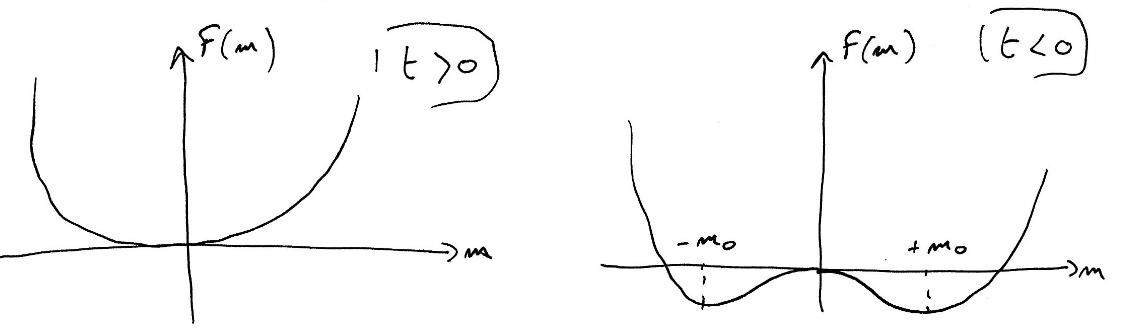
\includegraphics[width=.8\textwidth]{chapters/Figures/introduction/double_well.png}
    \caption{The double Landau free energy changes from a single to a double well as the control parameter is tuned past the critical point.}
    \label{fig: double well}
\end{figure}

%To go beyond the mean-field approach, we include spatial dynamics.
From now, the system magnetization will thus no more be a simple number, but a field that depends on space and time $m = m(\bm x,t)$.
Considering a small subvolume of the system $\rmd\bm x$, close enough to the transition we can thus reasonably assume that the associated `bulk' free energy is given by $f(m) \rmd\bm x$
with
%
\begin{align} \label{eq_eff_Landau_FE}
    f(m) = \frac{1}{2}\alpha \vartheta  m^2 + \frac{1}{4} \beta m^4,
\end{align}
%
where $\alpha \approx k_B T_c$ and $\beta \approx k_B T_c / 3 \approx \alpha / 3 $. 
Of course, we also need to account for the fact that $m$ cannot change arbitrarily fast between neighboring subvolumes, so that the presence of finite gradients must come at a cost.
%This is the ``Bulk free energy density''.
%The full free energy is the integral of this density, plus a term that takes into account the cost of gradients.
The simplest way to do this while preserving the invariance of the free energy under $m \to -m$ and rotations of space (which must always be obeyed as they are symmetries of the microscopic dynamics) is to include a term $\propto |\nabla m|^2$ in the free energy density.
Combining these terms together gives us the Ginzburg-Landau free energy functional\footnote{\emph{Functional}, not function, as $F[m]$ is a function of a function $m(\bm x)$. 
This means that the minimum of $F[m]$ is not determined by using derivatives $\odv{}{m}$, but functional derivatives $\fdv{}{m(\bm x)}$.}
%
\begin{align} \label{eq_GL_Ising}
    F[m] = \int \dd \bm x 
    \left(f(m) + \frac{1}{2} K |\nabla m|^2\right).
\end{align}
%

Analogously to the mean field analysis, the equilibrium magnetization profile minimizes the free energy~\eqref{eq_GL_Ising}. 
Namely, the associated condition is
$\delta F / \delta m(\bm x) = 0$, where the $\delta$ symbol indicates that we perform a functional derivative.
In fact, here we won't really be interested in the mean magnetization profile, but rather in characterizing the behaviour of the fluctuations around it.
One way to achieve this is to generalize the Langevin approach that we used in Sec.~\ref{intro_ABM} to model the dynamics of fields.
Namely, under the reasonable assumption that the force acting on $m$ derives from the free energy functional, we can write\footnote{We will see in Chapter~\ref{chap_thermo} how this form of the equation of motion gives the correct detailed-balance condition on the stochastic field dynamics.}
%To obtain a dynamical equation for this system, which governs the time-evolution of $m$, we assume purely dissipative dynamics, 
%
\begin{align} \label{eq_dyn_m_Ising}
    \partial_t m(\bm x, t)
    =
    - \fdv{F}{{m(\bm x, t)}} + \psi(\bm x, t)
    = - [\alpha \vartheta + \beta m^2(\bm x, t)] m(\bm x, t) + K \nabla^2 m(\bm x, t) + \psi(\bm x,t),
\end{align}
%
where $\psi$ is Gaussian white noise satisfying
%
\begin{align*}
    \E{\psi(\bm x, t)} &= 0, &
    \E{\psi(\bm x, t) \psi(\bm x', t')}
    = \Psi \delta(\bm x - \bm x') \delta(t - t').
\end{align*} 
%
Momentarily discarding the noise, Eq.~\eqref{eq_dyn_m_Ising} admits a homogeneous steady state solution $m_0$ given by
%
\begin{align*}
    (\alpha \vartheta + \beta m_0^2) m_0 = 0
    \implies
    \begin{cases}
        m_0 = 0, & \vartheta > 0, \\
        m_0 = \sqrt{ \frac{ \alpha |\vartheta| }{ \beta } }, & \vartheta \le 0,
    \end{cases}
\end{align*}
%
consistently with our previous analysis.
To study how this homogeneous solution is affected by the presence of fluctuations, we now write the magnetization field as $m(\bm x, t) = m_0 + \delta m(\bm x, t)$ and study the dynamics of $\delta m$ at the linear level.
The perturbation obeys the equation of motion
%
\begin{align} \label{eq_dm_Ising}
    \partial_t \delta m = - a^2 \delta m  + K \nabla^2 \delta m + \psi,
\end{align}
%
where the damping rate
%
\begin{align*}
    a^2 \equiv 
    \begin{cases}
        \alpha \vartheta, & \vartheta > 0, \\
        2 \alpha |\vartheta|, & \vartheta \le 0,
    \end{cases}
\end{align*}
%
is positive in both phases.
Because it is linear, Equation~\eqref{eq_dm_Ising} is easily solved in Fourier space, so that we define for any field $\phi(\bm x,t)$
%
\begin{align*}
    \hat \phi(\bm q, \omega)
    =
    \int \dd \bm x \dd t \, e^{i(\bm q \cdot \bm x + \omega t)} \phi(\bm x, t), \qquad
    \phi(\bm x, t)
    =
    \int \frac{\dd \bm q \dd \omega}{(2\pi)^{d+1}} \, e^{-i(\bm q \cdot \bm x + \omega t)}
    \hat \phi(\bm q, \omega).
\end{align*}
%
We then get
%
\begin{align}
    (i \omega + a^2 + Kq^2)\delta \hat m(\bm q,\omega) = \hat \psi(\bm q, \omega),
\end{align}
%
where $q = |\bm q|$ and the Fourier transform of the noise keeps a vanishing expectation value and has a covariance
%
\begin{align*}
    \E{\hat \psi(\bm q, \omega)\hat\psi(\bm q', \bm \omega')}
    = \Psi (2\pi)^{d + 1}\delta(\bm q + \bm q') \delta(\omega + \omega').
\end{align*}
%
With this, we easily can explicitly calculate the Fourier transform of the two-point correlation function,
%
\begin{align*}
    \hat C(\bm q, \bm \omega)
    = 
    \frac{\E{\delta \hat m(\bm q, \omega) \delta \hat m(-\bm q, -\omega)}}{(2\pi)^{d + 1}\delta(\bm q + \bm q') \delta(\omega + \omega')  }
    = 
    \frac{\Psi}{\omega^2 + (a^2 + K q^2)^2}.
\end{align*}
%
We obtain the equal-time correlation by integrating over all frequencies. Performing the integral\footnote{Using that 
$\int_{-\infty}^{+\infty} \tfrac{\dd x}{2\pi} \tfrac{1}{x^2 + a^2} = 
\tfrac{1}{2\pi a}\int_{-\infty}^{+\infty} \tfrac{\dd y}{y^2 + 1} = \tfrac{1}{2\pi a} [\arctan(y)]_{-\infty}^{+\infty}= \tfrac{1}{2a}$}, 
we get
%
\begin{align}
    \hat C(\bm q) \equiv \int\limits_{-\infty}^{+\infty} \frac{\dd \omega}{2 \pi} \hat C(\bm q, \omega)
    = 
    \frac{1}{2}\frac{\Psi }{a^2 + K q^2}.
\end{align}
%
The real space two-point correlation function is then
%
\begin{align}    \label{eq_CF_Ising}
    C(\bm x)
    = \E{\delta m(\bm 0) \delta m(\bm x)}
    & = \frac{\Psi}{2 K}
    \int \frac{\dd \bm q}{(2 \pi)^d} \frac{e^{-i\bm q \cdot \bm x}}{\xi^{-2} + q^2}
    = \frac{\Psi}{2 K}
    \int \frac{\dd q}{2 \pi} 
    \frac{q^{d-1}}{\xi^{-2} + q^2}
    I(\bm q \cdot \bm x),
    %\int \frac{\dd\Omega}{(2\pi)^{d-1}}   \frac{e^{-i q x \cos\theta}}{\xi^{-2} + q^2}, \nonumber \\
\end{align}
%
where we have introduced the \emph{correlation length}
%
\begin{align} \label{eq_corr_length}
    \xi \equiv \sqrt{ \frac{ K }{ a^2 } },
\end{align}
%
while $I(\bm q \cdot \bm x) = \int \tfrac{\dd\Omega_q}{(2\pi)^{d-1}} \exp(- i \bm q \cdot \bm x)$, and the integration is performed over all orientations of $\bm q$.
As expected from the symmetries of the problem, the correlation function $C(x)$ is isotropic, and measures how much, on average, fluctuations in the magnetization are correlated over a distance $x$. 
The correlation length $\xi$ basically measures the length scale over which these correlations are significant.
We may see this by taking the two limits of the integral~\eqref{eq_CF_Ising},
%
\begin{align*}
    C(x) \simeq
    \begin{cases}
        x^{2-d}, & x \ll \xi, \\
        x^{1-d/2} e^{- x / \xi}, & x \gg \xi.
    \end{cases}
\end{align*}
%
Therefore, over distances less than the correlation length, the correlations exhibit a slow algebraic decay, $C(x) \sim x^{2 - d}$, while over distances much larger than $\xi$ they are exponentially suppressed.

As $\xi \propto 1/\sqrt{ |\vartheta| }$ (see Eq.~\eqref{eq_corr_length}), the correlation length is finite in both the disordered and ordered phases.
On the other hand, when approaching the transition $\vartheta \to 0$ the correlation length diverges, and the correlations become \emph{scale free}.
$\vartheta = 0$ defines a \emph{critical point}, which corresponds to a parameter regime where the dynamics of fluctuations has no intrinsic length scale, which can be visualized directly \href{https://www.youtube.com/watch?v=lQxD1PinDbs}{from simulations}.

Another consequence of the divergence of $\xi$ is that the large scale physics at the critical point is independent of the microscopic details of the model.
This property is at the root of the powerful concept of \emph{universality} commonly used in condensed matter physics.
At a critical point, the only features that govern the relevant large scale physics are fundamental characteristics of a system like its symmetries, the conservation laws it obeys, and its dimensionality.
Systems sharing the same characteristics are said to belong to the same universality class, and are thus formally described by the same theory.

A critical point is characterized by a set of critical exponents, which describe how various observables behave in its vicinity.
Examples we have already met include
%
\begin{align}
    |m_0| &\sim |\vartheta|^\beta, &
    \xi & \sim |\vartheta|^{-\nu}, &
    C(x) & \sim x^{d - 2 + \eta},
\end{align}
%
with the mean field exponents $\beta = \nu = \tfrac{1}{2}$ and $\eta = 0$.
To obtain these values we have assumed that the typical fluctuations of $m$ around its mean $m_0$ are small, so that we obtained a linear equation for the perturbations.
As the critical point corresponds to the vanishing of the damping term in Eq.~\eqref{eq_dm_Ising}, 
we can however reasonably question the validity of this approximation.
%these mean field predictions are generally incorrect, because we have neglected the non-linearities in the equation, and we have not taken into account the effects of fluctuations.

In fact, the Ising model can be solved exactly in dimensions one and two, 
and the corresponding solutions (unsurprisingly) do not match the predictions of the mean field theory.
Namely, in one dimension the dynamics is dominated by entropy: spins have too few nearest neighbors for the alignment to compete with fluctuations, so that the system is disordered at any finite temperature.
In two dimensions, the mean field calculation only gives a qualitatively correct picture. 
The exact solution derived by Onsager~\cite{Onsager1944} indeed predicts the existence of a critical point at a finite $T_c$, but the exact exponents are different from their mean field values.  
A similar situation is found in three dimensions, although the absence of an exact solution imposes to determine the exponents numerically.
In the end, the mean field theory is only quantitatively valid in dimensions higher than $4$, while $d_c = 4$ is known has the upper critical dimension of the model.
The values of the critical exponents in $d \ge 2$ are reported in Table~\ref{table_Ising_exp}.

\begin{table}[!t]
    \centering
    \caption{Critical exponents of the Ising model. Those in $d=2$ are exact, the $d=3$ ones are obtained from numerical simulations~\cite{CampostriniPRE2002}, while those in $d \ge 4$ are follow from the mean field analysis.}
    \begin{tabular}{r|c c c}
        $d$ & 2 & 3 & $\ge 4$ \\
        \hline
        $\beta$ & $1/8$ & $0.32653(10)$ & $1 / 2$ \\
        $\nu$ & $1$ & $0.63012(16)$ & $1 / 2$ \\
        $\eta$ & $1/4$ & $0.03639(15)$ & $0$
    \end{tabular}   
    \label{table_Ising_exp}
\end{table}

\begin{figure}[!b]
    \centering
    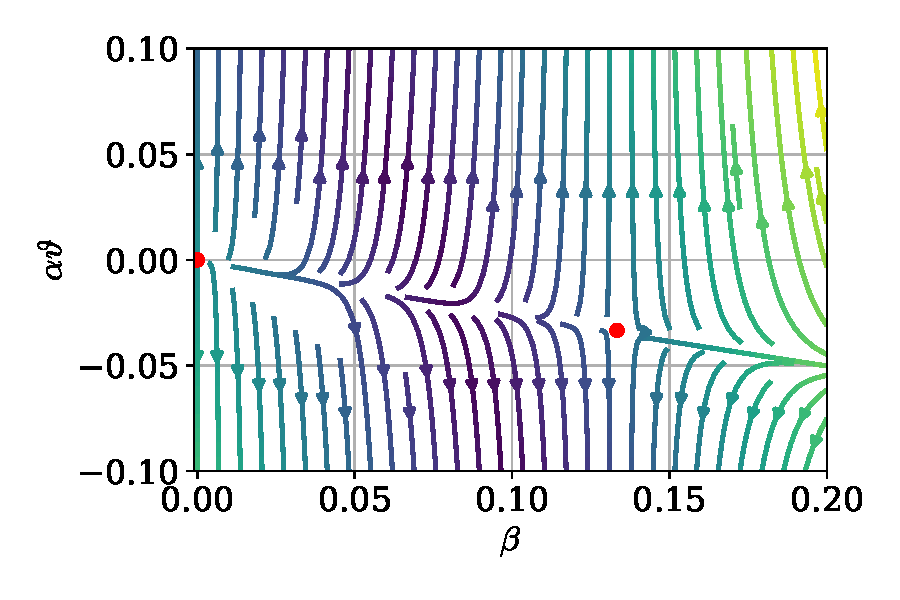
\includegraphics[width=.4\textwidth]{chapters/Figures/introduction/flow.pdf}
    \caption{
    %The flow in parameter space under renormalization group transformations.
        As the short wavelength physics is integrated out via renormalization group transformations, the theory is described by an effective free energy~\eqref{eq_GL_Ising} with a set of renormalized parameters.
        The the lines in this diagram indicate how the parameters of the theory `flow' under RG transformations.
        %values of the parameters $\alpha\vartheta$ and $\beta$ in~\eqref{eq_eff_Landau_FE} flow following the lines in this plot, which are given by the RG equations.
        The two red dots indicate fixed points where the theory is invariant under RG flow.
        }
    \label{fig: flow}
\end{figure}

A refined prediction for the value of the exponents in three dimensions requires to take into account the effect of nonlinearities, which can be done using the theoretical framework of the \emph{Renormalization Group} (RG).
%In fact, the one-dimensional Ising model can be solved exactly, and \emph{does not} feature a phase transition at finite temperature. In one dimension, there are too few nearest neighbors to keep spins ordered when thermal noise is introduced, and any non-zero temperature results in a finite correlation length.
%In the case of the Ising model, the mean-field breaks down for all dimensions lower than its \emph{critical dimension}, $d < d_c = 4$.
%To go beyond the mean field prediction and obtain accurate results for the critical exponents, one has to employ the \emph{Renormalization Group} or RG for short.
The RG framework relies on the scale invariance property of the critical point.
Its main idea is to study how the parameters of the free energy~\eqref{eq_GL_Ising} ($\alpha$, $\beta$ and $K$) renormalize as one changes the scale of the theory and integrates out the short wavelength physics. 
This approach leads to the RG equations, whose solutions tell us how the effective parameters of the theory `flow' as we investigate the physics over larger and larger scales. 
this is illustrated for the Ising model in \autoref{fig: flow}, where the parameters $\alpha \vartheta$ and $\beta $ follow the lines given by the RG equations.
The critical point then corresponds to a fixed point of these equations, meaning that the parameters do not change anymore with the scale of the theory: the physics is scale-free.
The red dot at $\alpha\vartheta = 0$ and $\beta = 0$ is the Gaussian fixed point that we have studied above.
This fixed point is unstable in dimensions $< 4$, so that in $d = 2$ and $d = 3$ the critical behavior of the Ising model is described by another fixed point at $\beta \neq 0$ (the other red dot in Fig.~\ref{fig: flow}), named the Willson-Fischer fixed point.
You can find a visual illustration of the RG flow \href{https://www.youtube.com/watch?v=MxRddFrEnPc}{here}.
A detailed introduction to RG, can be found in the textbook references~\cite{Goldenfeld1992,Kardar2007}. 



%In this method, one explicitly integrates out the short-wavelength dynamics.
%With this, one may derive equations describing how the parameters in the free energy, such as $\alpha$ and $\beta$ above, change as one changes the scale of the theory.
%These are the \emph{Renormalizatio Group Equations}.
%A fixed point in the RG equations means that the parameters do not change, and thus that the corresponding model is scale-free.
%Below we report some of the exponents for the Ising model.


%In 3 dimensions, one has to resort to renormalization or numerics.
%In the table below, we provide some the exponents in various dimensions.
%Those in 2D are exact, the 3D ones are from numerics, while those above 4D are the mean-field exponents.



\subsection*{Continuous symmetries: Goldstone modes and the Mermin-Wagner theorem}

At the beginning of this section, we motivated the present introduction on critical phenomena by mentioning the example of flocking.
Contrary to Ising spins which can only take discrete values, birds are free to move in any direction they please.
Hence, the self-propulsion direction of a bird is better described by a vector than a scalar.
Here, we will therefore stay within the framework of equilibrium systems, but make a step closer to actual birds by extending our analysis to systems presenting a continuous rotational symmetry.

%The Ising model has the discrete symmetry $s_i \rightarrow -s_i$, in mathematical terms $\mathbb{Z}_2$.
%The equations of motion, and thus all physics, remain unchanged if all spins are flipped upside-down.
%We will now consider spins that are free to rotate around, and not just point up or down so that the spin at each site is represented by a vector $\bm s_i$.

We therefore consider $N$ vector spins $\{\bm s_i\}$, each having $n$ components, on a lattice in $d$ dimensions.
The magnetization measuring the amount of order in the system is thus also a vector, 
%
\begin{align}
    \bm m = \frac{ 1 }{ N } \E{{\sum}_i \bm s_i},
\end{align}
%
while the energy function~\eqref{eq_energy_Ising} is generalized to
%
\begin{align} \label{eq_energy_ON}
    E = - \frac{J}{2} \sum_{\E{ij}} \bm s_i \cdot \bm s_j.
\end{align}
%
By construction, the energy~\eqref{eq_energy_ON} remains unchanged when one rotates all spins at the same time.
This class of transformations belongs to the orthogonal symmetry group $\mathrm{O}(n)$, so that the model defined by~\eqref{eq_energy_ON} is usually referred to as the $\mathrm{O}(n)$ model.
Note that the Ising model we studied previously corresponds to the particular case $n = 1$ (in this case the symmetry is of course discrete and amounts to flipping all spins),
while the $n = 2$ and $n = 3$ are respectively known as the $XY$ and Heisenberg models.

%This symmetry, which in group theory is called a $\mathrm{O}(n)$ symmetry where $n$ is the number of dimensions of the vector being rotated, is continuous.

We now generalize the Ginzburg-Landau approach presented in the previous section to this case with continuous symmetries.
Assuming again a regime where the amplitude of the vector $\bm m$ is small, we write a low-order expansion of the free energy that satisfies the $\mathrm{O}(n)$ symmetry:\footnote{
For simplicity, we have set $\alpha = \beta = 1$. This choice of parameters basically amounts to a specific choice of units for $\vartheta$ and $|\bm m|$.}
%
\begin{align} \label{eq_FE_ON}
    F = \int \dd \bm x \, 
    \left(
        \frac{\vartheta}{2}  |\bm m|^2 + \frac{1}{4} |\bm m|^4 + \frac{K}{2} |\nabla \bm m|^2
    \right),
\end{align}
%
where the gradient term should be understood as $|\nabla \bm m|^2 = \sum_{i, \alpha}\nabla_i m_\alpha \nabla_i m_\alpha$.
For $\vartheta > 0$, the bulk part of the free energy~\eqref{eq_FE_ON} corresponds to a single well centered at $\bm m = \bm 0$, while for $\vartheta < 0$ it has a continuum of degenerate minima satisfying $|\bm m| = \sqrt{|\vartheta|}$.
For $n = 2$, in particular, the free energy landscape takes the well-known Mexican-hat shape shown in Fig.~\ref{fig: mexican}.

\begin{figure}[!htb]
    \centering
    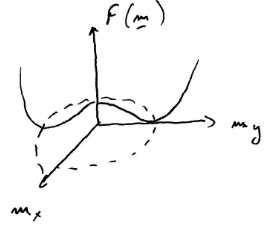
\includegraphics[width=.5\textwidth]{chapters/Figures/introduction/mexican.png}
    \caption{The Mexican-hat potential.}
    \label{fig: mexican}
\end{figure}

%Here, the gradient term represents a dot-product of both the gradients and the magnetization, $|\nabla m|^2 = \nabla_\alpha m_\beta \nabla_\alpha m_\beta$.
We now follow the same procedure as before, leading to the stochastic dynamics,
%
\begin{align}
    \partial_t \bm m = - (\vartheta + |\bm m|^2) \bm m + K \nabla^2 \bm m
    + \bm \psi,
\end{align}
where the noise $\bm \psi$ has zero mean and correlations
\begin{align*}
    \E{\psi_i(\bm x, t) \psi_j(\bm x', t')}
    = \Psi \delta_{ij} \delta^d(\bm x - \bm x') \delta(t - t') 
    \qquad \forall i,j \in [0;n].
\end{align*} 
%

As before, the steady-state solution of the deterministic equation
%
\begin{align*}
    |\bm m_0|^2 
    =
    \begin{cases}
        0, & \vartheta > 0 \\
        |\vartheta|, & \vartheta < 0 
    \end{cases}
\end{align*}
%
only defines the magnitude of the mean order, while its direction remains arbitrary and is picked at random by the system.
%Now, the steady-state solution is picked not from two degenerate minima, but instead from a continuum of degenerate minima.
We thus write the deterministic stationary solution as $\bm m_0 = m_0 \hat {\bm u}_\parallel$, where $\hat {\bm u}_\parallel$ is a $n$-dimensional unit vector giving the direction of the 
mean order.
We also expand $\bm m$ in terms of longitudinal and transverse perturbations
%
\begin{align*}
    \bm m &= (m_0 + \delta m_\parallel) \hat {\bm u}_\parallel + \delta \bm m_\perp,
\end{align*}
%
such that $\delta \bm m_\perp \cdot \hat {\bm u}_\parallel = 0$.
You can easily convince yourself that the analysis of the disordered phase $\vartheta > 0$ will not lead to any qualitatively new behavior w.r.t. what we have discussed for the Ising model, so here we will focus on analysing the ordered solution, i.e., taking $\vartheta < 0$.
The linearized equations for the perturbations are then
%
\begin{subequations}
\begin{align}
    \label{eq_ON_dmpara}
    \partial_t \delta m_\parallel 
    & = 
    2 t \delta m_\parallel + K \nabla^2 \delta m_\parallel + \psi_\parallel, \\
    \label{eq_ON_dmperp}
    \partial_t \delta \bm m_\perp
    & = K \nabla^2 \delta \bm m_\perp + \bm \psi_\perp,
\end{align}
\end{subequations}
%
where $\psi_\|$ and $\bm \psi_\perp$ correspond to projections of the noise along the longitudinal and transverse directions, and remain uncorrelated Gaussian white noises with variance $\Psi$.

Comparing Eqs.~\eqref{eq_dm_Ising} and~\eqref{eq_ON_dmpara},
it is clear that the longitudinal fluctuations are described by the same equation as for the Ising model, so that they are correlated over a finite correlation length $\xi_\| = \sqrt{ K / 2 |\vartheta| }$.
The dynamics of transverse perturbations, on the other hand, is not damped so that it is
associated with a diverging correlation length for all $\vartheta \le 0$.
The reason for this is quite intuitive: a uniform transverse perturbation $\delta\bm m_\perp$ corresponds to a global rotation of the mean order, which comes at zero energetic cost. 
Depending on who you are talking to, $\delta \bm m_\perp$ will be called a \emph{Goldstone mode}, a \emph{spin wave} or,
in the language of high-energy physics, a \emph{massless mode}.
%This results from the spontaneous breaking of a continuous symmetry. When this happens, there is no energetic cost associated with a global rotation. Consider the Mexican hat, given some direction of symmetry breaking, one can always rotate the corresponding unit vector around the center without incurring an energetic cost.

Goldstone modes are associated with the presence of a continuous symmetry, and their presence has important consequences.
First, the spatial correlations of the order parameter are scale-free:
%
\begin{align}
    \hat C_\perp(\bm q) = \frac{(n - 1)\Psi}{2 K q^2},
\end{align}
%
where the $(n-1)$ factor comes from the fact that the transverse fluctuation vector has $n-1$ components.
While observing the critical behavior of the Ising model required to fine tune $\vartheta$ to $0$, here criticality is present in the whole ordered phase.
Secondly, as fluctuations are essentially not damped at large scales, the question of how they affect the macroscopic order arises.
To quantify this, we calculate their typical amplitude $\E{|\delta\bm m_\perp|^2}$, which is obtained from the equal-time correlation function as
\begin{align} \label{eq_fluct_MW}
    \E{|\delta\bm m_\perp|^2} = 
    \int \frac{\dd\bm q}{(2 \pi)^d} \hat C_\perp(\bm q) 
    \propto \int\limits_{1 / L}^{1/a} q^{d - 3}
    \underset{L \to \infty}{\sim}
    \begin{cases}
        L^{2 - d}, & d < 2, \\
        \ln\frac{L}{a}, & d = 2, \\
        a^{2 - d}, & d > 2.
    \end{cases}
\end{align}
Here, we have introduced two cutoff scales in the last integration. 
$a$ serves as a microscopic (sometimes referred to as ultraviolet (UV), since it corresponds to short-wavelength fluctuations) cutoff and should be interpreted as the minimum scale beyond which the field theory can be considered valid\footnote{
In any dimensions, it is clear from Eq.~\eqref{eq_fluct_MW} that the magnetization fluctuations diverge as $a \to 0$.
However, the underlying approximation of the theory that describes the system  with smooth fields is only valid down to a finite scale set by, e.g., the lattice spacing or the typical particle size.
Below this microscopic scale, it is reasonable to suppose that the field theoretical description breaks down.
The UV divergence obtained by taking $a \to 0$ in~\eqref{eq_fluct_MW} is therefore unphysical, as it is an artifact introduced by the model assumptions, which is why we regularize it by hand.}. 
In general, $a$ will be (roughly) given by the lattice size.
The scale $L$ is macroscopic cutoff (sometimes referred to as infrared (IR), since it corresponds to long-wavelength fluctuations) that plays the role of the system size.

%By imposing a Lattice size, $a$ and a system size $L$, we get finite limits for our integral and consider the dominant behavior as we approach a continuous system, $a \rightarrow 0$, in the thermodynamic limit, $L \rightarrow \infty$,
%

For $d \le 2$, Eq.~\eqref{eq_fluct_MW} predicts that the amplitude of transverse magnetization fluctuations diverge in the thermodynamic limit where the system size becomes infinite.
%This is exactly the regime where we are hoping our model is a good description and not something we can sweep under the rug.
%In $d = 2$, the lower critical dimension for the $\mathrm{O}(N)$ model, the theory diverges both in the IR and the UV.
%The IR divergence is a physical prediction.
This result indicates that fluctuations of the Goldstone mode destroy order in all dimensions below 2. 
%What it tells us is that our assumption of a state that is mostly ordered, with small fluctuations $\bm m = \bm m_0 + \delta \bm m $ is wrong.
In other words, in dimensions $d \leq 2$, there cannot be long-range order associated with the spontaneous breaking of a continuous symmetry.
This feature is an instance of the so-called \emph{Mermin-Wagner theorem}.

\subsection*{Universality and active matter}

As we have just shown, for systems with continuous symmetries the concepts of scale invariance---and thus universality---are not only associated with phase transitions but also more generally with the emergence of macroscopic order.
Naturally, we expect these features to extend to certain out-of-equilibrium dynamics, and especially to active matter.
This, in particular, motivates the classification of active systems in terms of their symmetries and conservation laws which is used to structure this course.




    \chapter{Hydrodynamics - Lecture 3}
    \label{chap_hydro}
    As alluded to in \autoref{sec: hydrodynamics of microswimmers}, microswimmers are often immersed in a fluid, which we have to take into account in our models.
In this lecture, we will extend the analysis of hydrodynamics needed to model active particles.


\section{Stokes flow}

The interaction of microswimmers with a fluid is quite different to what we are used to at macroscopic scales.
To see the effect of scales on the hydrodynamics, we begin with the most general equations for a fluid, the Navier-Stokes equation, and show that in certain regimes, this reduces to the much simpler Stokes equation.
Hydrodynamic flows where this is the case are called Stokes flows, and as we will show, this is the relevant regime for microswimmers.

\subsection{Navier-Stokes equations}

We start with the hydrodynamic equation with inertia
\begin{align}
    \rho\left(
    \frac{\partial \mathbf{v}}{\partial t}
+\mathbf{v}\cdot\nabla\mathbf{v}
    \right)
    =\eta\nabla^2\mathbf{v}
    -\nabla p +\rho\mathbf{f},
    \label{eq:NS}
\end{align}
with $\rho$ density, $\mathbf{v}$ velocity field, $\eta$ viscosity, $p$ pressure, and $\rho\mathbf{f}$ force density.
The first term on the LHS varies with time and the second represents convection, while the first term on the RHS results from dissipation and the second represents force due to the pressure gradient.
If fluids cannot be compressed, the continuity equation holds
\begin{align}
    \frac{\partial \rho}{\partial t}
    + \nabla\cdot(\rho\mathbf{v})=0.
\end{align}


Taking the ratio of the second term on the LHS of Eq.~(\ref{eq:NS}) and the first term on the RHS gives the Reynolds number
\begin{align}
    \frac{\rho V^2/a}{\eta V/a^2}
    =
    \frac{\rho V a}{\eta}
    \equiv {\rm Re},
\end{align}
where $V$ is a characteristic velocity and $a$ is a typical size relevant to microswimmers.
On the other hand, taking the ratio of the first term on the LHS of Eq.~(\ref{eq:NS}) and the first term on the RHS leads to the Strouhal number:
\begin{align}
    \frac{\rho V/\tau}{\eta V/a^2}
    =
    \frac{\rho a^2/\eta}{\tau}
    \equiv {\rm Re}\cdot{\rm St},
\end{align}
where the characteristic timescale is chosen as $\tau$.
Using typical values such $\rho\sim1000~{\rm kg}\cdot{\rm m}^{-3}$ (water), $a\sim1~\mu{\rm m}$, $\eta\sim10^{-3}~{\rm Ps}\cdot{\rm s}$ (water), and $V\sim10$ body length per second, one can obtain ${\rm Re}\sim10^{-5}$ and ${\rm Re}\cdot{\rm St}\sim10^{-6}~{\rm s}/\tau$.



\subsection{Stokes equations}

At zero Reynolds number, the governing equations become
\begin{align}
    \eta\nabla^2\mathbf{v}-\nabla p +\rho\mathbf{f}=\mathbf{0}, \quad
    \nabla\cdot\mathbf{v}=0.
\end{align}
It is worth noting that 
\begin{itemize}
    \item no time dependence in the equations
    \item fluids responds to any change in the boundary condition instantly
    \item equations are linear in the velocity and hence kinematic reversibility holds.
    \item Scallop theorem holds, which states that in order for a microswimmer to swim using cyclic deformations, more than two decrees of freedom is necessary.
\end{itemize}
The Scallop theorem was proposed in E.\ M.\ Puercell, Am.\ J.\ Phys.\ (1977) and was later mathematically proved in Ishimoto and Yamada, SIAM Journal on Applied Mathematics (2012).


\subsection{How to circumvent the Scallop theorem?}

For example, inertialess single rigid swimmers cannot show net motion by undergoing reciprocal body distortions. But some flexibility leads the swimmers to show motion. This can be seen in a bacterium, which has a single helix and seems that only one degree of freedom exists. 
The fact that it can swim is explained by the flexibility of the flagella attached to the body. Another simple model is the three-sphere microswimmer proposed by Najafi and Golestanian in 2004, which is composed of three spheres connected by rigid shafts.


\subsection{Passive hydrodynamic problem}

\todo[inline]{add motivation/figure for problem}

We consider a passive (forced) rigid particle in viscous fluids, which moves with translational velocity $\mathbf{V}$ and rotational velocity $\boldsymbol{\Omega}$. 
The velocity induced by this particle obeys the Stokes equations
\begin{align}
    \eta\nabla^2\mathbf{v}-\nabla p =\mathbf{0}, \quad
    \nabla\cdot\mathbf{v}=0,
    \label{eq:stokes}
\end{align}
with the no-slip boundary condition at the surface
\begin{align}
    \mathbf{v} = \mathbf{V}+\boldsymbol{\Omega}\times\mathbf{r}.
\end{align}
Here background flows are set to be zero, i.e., $\mathbf{v}=\mathbf{0}$ for $r\to\infty$.
In this setup, the external force acting on the particle is balanced by the drag exerting from a medium:
\begin{align}
    \mathbf{F}+\mathbf{F}_{\rm D}= \mathbf{0}.
\end{align}
The force acting from the fluid can be calculated by integrating the traction over the object surface
\begin{align}
    \mathbf{F}_{\rm D}
    =
    \int_{\rm S}dS\, \boldsymbol{\sigma}\cdot\mathbf{n},
\end{align}
where the second-rank stress tensor of a Newtonian fluid is given by $\boldsymbol{\sigma}=-p\mathbf{I}+\eta(\nabla\mathbf{v}+\nabla\mathbf{v}^T)$ and $\mathbf{n}$ is a surface normal pointing into the fluid.


In the following, we shall derive Stokes' law for a translating sphere, which is a basic hydrodynamic problem solved by George Gabriel Stokes. 
The law states that the force acting on a sphere (radius $a$) moving with velocity $\mathbf{V}$ in a medium of viscosity $\eta$ is expressed with
\begin{align}
    \mathbf{F}_{\rm D}= -6\pi\eta a \mathbf{V}.
\end{align}


We start with obtaining the pressure expression. Taking the divergence of Eq.~(\ref{eq:stokes}) gives $\nabla^2p=0$, implying the pressure is harmonic. Possible solutions are $1/r$ and its spatial derivatives such as $\mathbf{r}/r^3$ (source), $\mathbf{I}/r^3-3\mathbf{rr}/r^5$ (source dipole), and so on. 
From the fact that the pressure is a scalar and the equations~(\ref{eq:stokes}) are linear in the velocity, one can infer that the pressure takes the form of
\begin{align}
    p(\mathbf{r})= c_1 \frac{\mathbf{r}\cdot\mathbf{V}}{r^3}.
\end{align}


In order to solve the velocity $\mathbf{v}$, one can decompose the Stokes equation~(\ref{eq:stokes}) into the homogeneous $\mathbf{v}_{\rm h}$ and particular solutions $\mathbf{v}_{\rm p}$, where $\nabla^2\mathbf{v}_{\rm h}=\mathbf{0}$. 
Again from the similar arguments, since the velocity is a vectorial quantity and is linearly proportional to $\mathbf{V}$, the homogeneous solution is constructed by a source and source dipole
\begin{align}
    \mathbf{v}_{\rm h} =  
    c_2 \frac{\mathbf{V}}{r}
    +
    c_3 \left(
    \frac{\mathbf{I}}{r^3}-\frac{3\mathbf{rr}}{r^5}
    \right)\cdot\mathbf{V}.
\end{align}
The particular solution can be obtained from the expression $\eta\nabla^2\mathbf{v}_{\rm p}-\nabla p=\mathbf{0}$.
Through the relation $\nabla^2(\mathbf{r}p)=2\nabla p$, the Stokes equation can be rewritten as
\begin{align}
    \eta\nabla^2 
    \left(
    \mathbf{v}_{\rm p}-
    \frac{1}{2\eta}\mathbf{r}p
    \right)=\mathbf{0},
\end{align}
which yields $\mathbf{v}_{\rm p}=\mathbf{r}p/(2\eta)$.


Having obtained the velocity and pressure, one finds the velocity follows
\begin{align}
    \mathbf{v}=
    \frac{1}{r}
    \left(
    c_2 + \frac{c_3}{r^2}
    \right)
    \mathbf{V}
    +
    \frac{1}{r}
    \left(
    \frac{c_1}{2\eta}\frac{\mathbf{rr}}{r^2}
    -
    c_3 
    \frac{3\mathbf{rr}}{r^4}
    \right)
    \cdot
    \mathbf{V}.
\end{align}
From the boundary condition, one finds
\begin{align}
    \mathbf{v}=
    \left(
    \frac{3a}{4r} + \frac{a^3}{4r^3}
    \right)
    \mathbf{V}
    +
    \left(
    \frac{3a}{4r^3}
    -
    \frac{3a^3}{4r^5}
    \right)
    \mathbf{rr}
    \cdot
    \mathbf{V}.
    \label{eq:sphere}
\end{align}


\todo[inline]{add velocity plot}

\subsection{Oseen tensor: the linear hydrodynamic response due to a point force}


By solving the forced Stokes equation, we derive the corresponding Green's function, which is known as the Oseen tensor.
One can obtain this propagator from the solution to the flow problem around a sphere.
For a point force at the origin, its induced velocity is calculated from Eq.~(\ref{eq:sphere}) when two neighboring spheres have vanishing small radii, i.e., in the limit of $a\to0$
\begin{align}
    \mathbf{v}(\mathbf{r})
    =
    \frac{1}{8\pi\eta r}
    \left(
    \mathbf{I} +\frac{\mathbf{rr}}{r^2}
    \right)
    \cdot
    \mathbf{F},
\end{align}
where $\mathbf{F}= 6\pi\eta a \mathbf{V}$ has been used.


\section{Active hydrodynamic problem}


\subsection{Hydrodynamic flow around an active particle}


In general, the far-field from around an object immersed in a fluid of viscosity $\eta$ can be expressed with
\begin{align}
    v_i(\mathbf{r})
    =
    \frac{1}{8\pi\eta}G_{ij}F_j
    -
    \frac{1}{8\pi\eta}C_{ij}T_j
    +
    \frac{1}{16\pi\eta}
    K_{ijk}S_{jk}
    +\dots,
\end{align}
where $\mathbf{F}$ is the force, $\mathbf{T}$ is the torque, and $\mathbf{S}$ is the symmetric tensor called stresslet with $\mathbf{C}$ and $\mathbf{K}$ being, respectively, the symmetric and anti-symmetric part of the derivative of the Oseen tensor $\mathbf{G}$.
One can see that the velocity, to the leading order, decays with a power of $r^{-1}$, while the other terms above decreases faster as $r^{-2}$.
For active or living particles, the force-free and torque-free conditions should hold, namely, $\mathbf{F}=\mathbf{T}=\mathbf{0}$. Hence, the leading contribution decays as $r^{-2}$.

Stresslet or symmetric force dipole characterizes the flow induced by a microswimmer. 
For a trace-free and symmetric second-rank tensor, the stresslet is written as $\mathbf{S}=\alpha(\mathbf{e}\otimes\mathbf{e}-\mathbf{I}/3)$ with direction $\mathbf{e}$.
The sign of the parameter $\alpha$ determines the type of microswimmers: $B_2 > 0$ corresponds to pullers, which generate thrust from the front, while $B_2 < 0$ corresponds to pushers, which generate thrust from the back. Swimmers with $\alpha=0$ are neutral swimmers.



\subsection{Squirmer model}

\todo[inline]{Hsould have illustration}


Here we consider a simple model of microswimmers with surface activity, such as ciliated microorganisms. By assuming that cilia are smaller than body size and all activity takes place in the narrow regime at the surface, one can replace them with effective slip velocity.
Such a model is called squirmer model and was first proposed by Lighthill (1952) and later developed by Blake (1971).
If we denote by $\mathbf{v}_{\rm s}$ the effective surface velocity, the velocity in the laboratory frame is given by $\mathbf{v}=\mathbf{V}+\boldsymbol{\Omega}\times\mathbf{r}+\mathbf{v}_{\rm s}$ at the object surface.

\todo[inline]{should have an explenation of what the theorem says.}

We can now make use of the Lorentz reciprocal theorem to calculate the propulsion velocity directly from the surface slip (see the next subsection for the derivation).
\begin{align}
    \int_\mathcal{S} dS\,
    \mathbf{v}\cdot\hat{\boldsymbol{\sigma}}
    \cdot\mathbf{n}
    =
    \int_\mathcal{S} dS\,
    \hat{\mathbf{v}}\cdot\boldsymbol{\sigma}
    \cdot\mathbf{n}
    .
    \label{eq:LRT}
\end{align}
Let us now choose $(\mathbf{v},\boldsymbol{\sigma})$ to be the force-free and torque-free motion of an object with a surface slip velocity boundary condition, and $(\hat{\mathbf{v}},\hat{\boldsymbol{\sigma}})$ to describe the motion of the same object when dragged through the viscous fluid by an external force $\hat{\mathbf{F}}$ with velocity $\hat{\mathbf{V}}$.
Since $\hat{\mathbf{v}}=\hat{\mathbf{V}}$ at the surface and solution is force-free, the right hand side of Eq.~(\ref{eq:LRT}) vanishes. 
Inserting $\mathbf{v}$ without the angular velocity into the theorem gives
\begin{align}    
    \mathbf{V}\cdot
    \hat{\mathbf{F}}
    =
    -
    \int_\mathcal{S} dS\,
    \mathbf{v}_{\rm s}\cdot\hat{\mathbf{f}}.
\end{align}
For a sphere of radius $a$, we have $\hat{\mathbf{f}}=\hat{\mathbf{F}}/(4\pi a^2)$, from which the drift velocity of a spherical squirmer follows
\begin{align}
    \mathbf{V}=- \frac{1}{4\pi a^2} \int_S dS\, \mathbf{v}_{\rm s}.
\end{align}
Similarly, the angular velocity of a spherical particle is obtained as
\begin{align}
    \boldsymbol{\Omega} =
    - \frac{3}{8\pi a^3} \int_S dS\, \mathbf{n}\times\mathbf{v}_{\rm s}.
\end{align}
In general, the tangential surface velocity can be expanded in the basis of Legendre polynomials as $v_\theta=\sum_{n=1} 2B_n/[n(n+1)]\sin\theta P_n^\prime(\cos\theta)$.
One can show that the slip velocity should have a nonvanishing first harmonic in order for an axisymmetric squirmer to lead to a translational velocity. 
Specifically, the swimmer with direction $\mathbf{e}$ moves with $\mathbf{V}=(2/3)B_1\mathbf{e}$.



\subsection{Lorentz reciprocal theorem}


Here we provide a general form of the reciprocal theorem for a two-phase compressible flow with body force.
Let the unhatted and hatted symbols represent the variables for any two arbitrary types of flows that satisfy the following equations:
\begin{align}
    \partial_j\sigma_{ij}+\mathfrak{f}_i=0,\quad
    \partial_j\hat{\sigma}_{ij}+\hat{\mathfrak{f}}_i=0,
    \label{eq:body}
\end{align}
where $\sigma_{ij}=-p\delta_{ij}+\eta_{ijk\ell}\partial_\ell v_k$ and $\hat{\sigma}_{ij}=-\hat{p}\delta_{ij}+\hat{\eta}_{ijk\ell}\partial_\ell\hat{v}_k$ are the stress tensors with the pressure field $p$, the identity tensor $\delta_{ij}$, the viscosity tensor $\boldsymbol{\eta}$, the velocity field $\mathbf{v}$, and the arbitrary body force density $\boldsymbol{\mathfrak{f}}$.
The inner product of $\mathbf{v}$ with the second expression in Eq.~(\ref{eq:body}) gives
\begin{align}
    \partial_j (\hat{\sigma}_{ij}v_i)+\hat{p}\partial_iv_i
    -\hat{\eta}_{k\ell ij}(\partial_\ell v_k)(\partial_j\hat{v}_i)
    + \hat{\mathfrak{f}}_iv_i = 0,
    \label{eq:hatted0}
\end{align}
and the equivalent expression with $\boldsymbol{\sigma}$ and $\hat{\mathbf{v}}$
\begin{align}
    \partial_j (\sigma_{ij}\hat{v}_i)+p\partial_i\hat{v}_i
    -\eta_{ijk\ell}(\partial_\ell v_k)(\partial_j\hat{v}_i)
    + \mathfrak{f}_i\hat{v}_i = 0.
    \label{eq:unhatted0}
\end{align}
In classical fluids, the viscosity tensor is composed solely of its symmetric components with respect to swapping the indices $ij\leftrightarrow k\ell$, namely,
\begin{align}
    \eta_{ijk\ell}= \eta_{k\ell ij}.
\end{align}
Based on this symmetry argument, we find from Eqs.~(\ref{eq:hatted0}) and (\ref{eq:unhatted0})
\begin{align}
    \partial_j (\hat{\sigma}_{ij}v_i)+\hat{p}\partial_iv_i
    -\hat{\eta}_{ijk\ell}(\partial_\ell v_k)(\partial_j\hat{v}_i)
    + \hat{\mathfrak{f}}_iv_i &= 0, \label{eq:hatted}\\
    \partial_j (\sigma_{ij}\hat{v}_i)+p\partial_i\hat{v}_i
    -\eta_{ijk\ell}(\partial_\ell v_k)(\partial_j\hat{v}_i)
    + \mathfrak{f}_i\hat{v}_i &= 0. \label{eq:unhatted}
\end{align}
If we allow for the linear relation between the two tensorial quantities, i.e., $
\hat{\boldsymbol{\eta}}=c\boldsymbol{\eta}$ with a constant $c$ and subtract Eq.~(\ref{eq:unhatted}) from Eq.~(\ref{eq:hatted}), we obtain
\begin{align}
    \partial_j (\hat{\sigma}_{ij}v_i)+\hat{p}\partial_iv_i + \hat{\mathfrak{f}}_iv_i
    =
    c[
    \partial_j (\sigma_{ij}\hat{v}_i)+p\partial_i\hat{v}_i + \mathfrak{f}_i\hat{v}_i
    ]
    .
\end{align}
Integrating over the fluid volume $\mathcal{V}$ and using the divergence theorem to obtain corresponding surface integrals over all bounding surfaces $\mathcal{S}$, the generalized reciprocal theorem is derived as
\begin{align}
    \int_\mathcal{S} dS\,
    \mathbf{v}\cdot\hat{\boldsymbol{\sigma}}
    \cdot\mathbf{n}
    -
    \int_\mathcal{V} dV\,
    (
    \hat{p}
    \nabla\cdot\mathbf{v}
    +
    \hat{\boldsymbol{\mathfrak{f}}}
    \cdot\mathbf{v}
    )
    =
    c
    \left[
    \int_\mathcal{S} dS\,
    \hat{\mathbf{v}}\cdot\boldsymbol{\sigma}
    \cdot\mathbf{n}
    -
    \int_\mathcal{V} dV\,
    (
    p
    \nabla\cdot\hat{\mathbf{v}}
    +
    \boldsymbol{\mathfrak{f}}
    \cdot\hat{\mathbf{v}}
    )
    \right]
    ,
\end{align}
where $\mathbf{n}$ is a surface normal pointing into the fluid.
For incompressible fluids with $c=1$ and without body forces, the Lorentz reciprocal theorem reduces to Eq.~(\ref{eq:LRT}).

    \chapter{Thermodynamics - Lecture 4}
    \label{chap_thermo}
    %%%%%%%%%%%%%
% Lecture 4 %
%%%%%%%%%%%%%

In this lecture, we give an overview of the thermodynamic tools that we have at our disposal for the characterization of active matter. 
As mentioned in Lecture 1, active matter defies thermodynamic equilibrium at the local scale. Some of the consequences of this property are: (i) the absence of a minimization principle for the steady-state statistics; (ii) the breaking of time-reversal symmetry of the steady-state dynamics; (iii) the absence of a generic thermodynamic framework. These are all related, as we will demonstrate shortly, via the concept of entropy production, which provides a measure of ``distance'' from equilibrium.


\section{Guessing the arrow of time}

Imagine being given the equation of motion of a particular process, after which a video of a sample realization of said process starts playing. How can you guess whether the video is currently being played in its original form, or whether it has been reversed?

Optimal decision theory, in particular Wald's ratio test \cite{PhysRevLett.115.250602}, tells us that the best time to make a guess between two competing hypotheses (here F=forward movie, B=backward movie) is the first occurrence of the quantity 
%
\begin{equation}\label{eq:Q_def}
    Q = \ln \frac{P(F|O)}{P(B|O)}
\end{equation}
%
reaching either of the pre-defined values $\pm Q^*$ (i.e. it is a first passage problem),
where $P(F,B|O)$ denote the posterior probability of either F or B being true given an observed realization $O$ of the process. We can equivalently write,
%
\begin{equation}
    P(F|O) = \frac{1}{2} + \frac{\tanh(Q)}{2},\quad P(B|O) = \frac{1}{2} - \frac{\tanh(Q)}{2}~,
\end{equation}
%
whereby $Q^*$ can be translated into a given degree of confidence about our guess. Using Bayes' theorem,
%
\begin{equation}
    P(F|O) = \frac{\mathbb{P}(O|F)P(F)}{\mathbb{P}(O)}
\end{equation}
%
and similarly for $P(B|O)$,
where we introduced the notation $\mathbb{P}$ to highlight the fact that these are ``path probabilities'' associated with a particular trajectory $O = \{o(t)\}_0^\tau$ of duration $\tau$. We set our prior probabilities $P(F) = P(B) = 1/2$ and substitute into \eqref{eq:Q_def} to obtain
%
\begin{equation}\label{eq:Q_def_paths}
    Q[O = \{o(t)\}_0^\tau] = \ln \frac{\mathbb{P}(O|F)}{\mathbb{P}(O|B)}~.
\end{equation}
%
Now, since all possible sample trajectories, whether played backward or not, originate from the original dynamics, we conclude that $\mathbb{P}(O|B) = \mathbb{P}(\hat{\Omega} O|F)$ with $\hat{\Omega}$ the time-reversal operator, i.e. the probability of being shown a particular trajectory O \emph{given that it was time-reversed} is simply the probability of the corresponding time-reversed trajectory $\hat{\Omega}O$ in the forward ensemble. It should be noted that the operator $\hat{\Omega}$ acts differently on different types of observables, depending in particular on their \emph{signature} under time-reversal: even quantities, such as densities and position, are invariant under time-reversal, while odd quantities, such as velocities and magnetic fields, change sign.

The quantity $Q[O]$ appearing in \eqref{eq:Q_def_paths} is a random variable, being a functional of a random path. To determine the mean rate with which confidence about our guess of the arrow of time is built, we average with respect to the ensemble of possible observed trajectories and divide by the trajectory duration
%
\begin{equation}
    \dot{\bar{Q}} \equiv \frac{\bar{Q}}{\tau} = \frac{1}{\tau} \int \mathcal{D}O \ \mathbb{P}(O|F) \ln \frac{\mathbb{P}(O|F)}{\mathbb{P}(O|B)}~.
\end{equation}
%
The structure in the right-hand side can be recognized as the Kullbeck-Leibler divergence \cite{kullback1951information} per unit time of the forward and time-reversed ensembles. This is a standard measure of statistical distinguishibility, vanishing when the two path probability distributions are identical. \\

Let us now compute this quantity for a simple case, specifically one-dimensional Brownian motion in the presence of an external position-dependent force. The governing Langevin equation reads
%
\begin{equation}
    \dot{x}(t) = \mu F(x(t)) + \sqrt{2k_B T \mu} \eta(t)
\end{equation}
%
where $\eta$ is a zero-mean Gaussian white noise of unit covariance, $\langle \eta(t)\eta(t')\rangle = \delta(t-t')$. In discrete time,
%
\begin{equation}
    dx_t = \mu F(x_t) dt + \sqrt{2k_B T \mu dt} \eta_t
\end{equation}
%
with $\eta_t \sim \mathcal{N}(0,1)$ now a set of iid zero-mean, unit variance Gaussian random variables. Thus, the probability of a particular realization of the noise has a simple factorized form,
%
\begin{equation}
    \mathbb{P}[\{\eta_t\}] \propto \prod_{i=0}^{\tau/dt} {\rm exp}\left( - \frac{\eta_i^2}{2} \right) 
    = {\rm exp}\left( - {\sum}_i \frac{\eta_i^2}{2} \right)~.
\end{equation}
%
Given a particular initial condition $x(0)$, any trajectory $x(t \in [0,\tau])$ is uniquely defined by the corresponding noise realisation $\eta(t \in [0,\tau])$. Thus, for an observable $A[x(t)]$ depending on $x(t)$ we can write expectations as
%
\begin{equation}
    \langle A \rangle = \int \mathcal{D}\eta \ \mathbb{P}[\eta] A[x[\eta]] = \int \mathcal{D}x \ \underbrace{\mathbb{J}[x] \tilde{\mathbb{P}}[x]}_{\mathbb{P}[x]} A[x]
\end{equation}
%
where we have performed a change of variable by including the relevant Jacobian $\mathbb{J}[x] \equiv \mathcal{D}\eta/\mathcal{D}x$. Whether the latter is a trivial quantity or not, depends on the implicit convention about the interpretation of the relevant stochastic integrals (Ito vs Stratonovich, or generalizations thereof \cite{tauber2014critical}). This discussion falls beyond the scope of this course so we sweep this difficulty under the carpet and simply take for granted that $\mathbb{J}[x] = \mathbb{J}[\hat{\Omega}x]$ is invariant under time-reversal and that the Stratonovich mid-point convention can be assumed when looking at products of random variables (the only discretization that allows for straightforward use of the standard chair rule of calculus). With all these caveats out of the way, we may write
%
\begin{equation}
    \mathbb{P}[x|F] \propto {\rm exp}\left( - \frac{1}{2} \sum_i \frac{(dx_t - \mu F(x_t)dt)^2}{2k_B T \mu dt} \right) \propto {\rm exp}\left( - \frac{1}{4k_B T \mu} \int dt\  [\dot{x}(t) - \mu F(x(t))]^2 \right)
\end{equation}
%
having taken the continuum limit $dt \to 0$. Recalling that positions and velocities are even and odd under time-reversal, respectively, we then have
%
\begin{align}
    \mathbb{P}(x|B) \propto {\rm exp}\left( - \frac{1}{4k_B T \mu} \int dt\  [-\dot{x}(t) - \mu F(x(t))]^2 \right)
\end{align}
%
whence
%
\begin{equation}\label{eq:q_vs_eqr}
    \dot{\bar{Q}} = \frac{\langle \dot{x}(t) F(x(t))\rangle}{k_B T}~. 
\end{equation}
%
Note how the numerator in the right-hand side of this expression is a product of the particle velocity times the force applied to it, and can thus be interpreted as the stochastic work done per unit time on the particle by the external force \cite{sekimoto1998langevin}. At steady-state, due to the conservation of energy, that same power needs to be dissipated as heat into the bath providing the thermal fluctuations. This quantity is thus nothing but the rate of entropy generation in the heat reservoir, $ \dot{\bar{Q}} = \dot{\sigma}$. This is a sign of the profound connection between entropy production as an informatic measure of time-reversal symmetry breaking, and its more traditional thermodynamic interpretation \cite{gaspard2004time}. In the following sections, we will follow a more traditional, i.e.\ thermodynamic, path for the derivation of this quantity.

Before moving on, let us note one important property of \eqref{eq:q_vs_eqr}. For conservative forces originating from an external potential that is bounded below and constant in time, $F(x) = -\partial_x U(x)$, we have by the chain rule that $\langle \dot{x}(t) F(x(t))\rangle = -\langle \dot{U} \rangle = 0$. In other words, the steady-state of Brownian dynamics in a stable potential is equilibrium/time-reversal symmetric. 



% Handwritten notes section (2)

\section{Gibbs-Shannon entropy (axiomatically)}

We briefly motivate the form of the Gibbs-Shannon entropy, which we will use in the following section. This can be derived ``axiomatically'' by imposing the following requirements on the thermodynamic entropy $S(\{p_i\}_{i=1,...,M})$ of a statistical ensemble, assuming for simplicity a discrete state space:

\begin{enumerate}
    \item For separate systems A and B treated as a single system, $S(A \cup B) = S(A) + S(B)$. Statistically speaking, the systems being ``separate'' or ``non-interacting'' means that the joint probability $p(a \in A, b \in B) = p(a)p(b)$ factorises ;
    \item Continuity/smoothness with $p_i$;
    \item $S(\{p_i\})$ should have a minimum $S=0$ when $p_i = 1$, $p_{j\neq i} = 0$ for some $i$;
    \item $S(\{p_i\})$ should have a positive maximum when $p_i = 1/M$ for all $i$.
\end{enumerate}
The Gibbs-Shannon entropy satisfies all these constraints,
%
\begin{equation}
    S_{GS} = -k_B \sum_i p_i \ln p_i~.
\end{equation}
%
The ``modern'' view of thermodynamics ({\`a} la Callen) takes the entropy as the fundamental quantity. For example, the ideal gas equations of state can be derived from the Sackur-Tetrode entropy
%
\begin{equation}
    S = \frac{3}{2}N k_B \ln \epsilon + N k_B \ln V + N k_B \left[ \ln\left( N^{-1} \left( \frac{4\pi m}{2Nh^2}\right)^{\frac{3}{2}} + \frac{5}{2} \right) \right]~,
\end{equation}
%
with intensive quantities following from suitable differentiation, e.g.
%
\begin{equation}
    P \equiv T \frac{\partial S}{\partial V} = \frac{Nk_B T}{V}~.
\end{equation}
%
% Handwritten notes section (2)
Similarly, the Boltzmann distribution of equilibrium thermodynamics, which applies to open systems coupled to a heat reservoir, can be obtained by maximizing the Gibbs-Shannon entropy while keeping the mean energy fixed (max-ent principle). In particular, one can check that $p_i \propto e^{-\beta E_i}$ with $\beta^{-1} = k_B T$ maximises the functional
%
\begin{equation}
    \mathcal{L}[\{p_i\}] = -k_B \sum_{i} p_i \ln p_i + \lambda_1 \left(\sum_i E_i p_i - \epsilon \right) + \lambda_2 \left(\sum_i p_i - 1 \right) 
\end{equation}
%
where $\epsilon = \langle E_i \rangle$ is the mean energy, while $\lambda_1$ and $\lambda_2$ are Lagrange multipliers enforcing the constraint on the mean energy and normalization, respectively.



\section{Entropy production rate from Gibbs-Boltzmann entropy}

% Handwritten notes section (4)

We now demonstrate how a formula analogous to \eqref{eq:q_vs_eqr} can be derived from thermodynamic, rather than informatic, considerations, taking the Gibbs-Boltzmann entropy as a starting point. 
%The entropy production rate (EPR) is exactly what it sounds like, the amount of entropy produced per unit of time.
Given a system that evolves stochastically with time, which we assume to be discrete for simplicity, we can write the Markov master equation
%
\begin{align}
    \odv{  }{ t } P_i(t) = K_{ij} P_j(t),
\end{align}
%
where $K_{ij}$ denotes the (Poisson) rate of transitioning from state $j$ to state $i$. The transition rates must obey $\sum_i K_{ij} = 0$ to conserve probability.
The corresponding Gibbs-Shannon entropy is
%
\begin{align}
    S(t) = - \sum_i P_i(t) \ln P_i(t),
\end{align}
%
which allows us to directly compute the rate of change of the entropy
%
\begin{align}
    \odv{  }{ t } S(t)
    \equiv \dot S(t)
    & = - \underbrace{{\sum}_i \dot P_i(t)}_{= 0}
    + - \sum_i \dot P_i(t) \ln P_i(t)\\
    & = 
    -\frac{1}{2}\sum_{ij}
    \left(
        K_{ij}P_j \ln P_i
        + K_{ji} P_i \ln P_j
    \right) 
\end{align}
%
where we have inserted the master equation, and rewritten the sum as two copies where the dummy indices are renamed. Assuming that a statistical steady-state exists, we have that $\lim_{t \to \infty} \dot{S}(t)=0$ and in this limit $P_i$ converges to the eigenvector of $K$ with eigenvalue zero.
With some more massaging, we can write this as
%
\begin{align}
    \dot S(t) &=
    -\frac{1}{2}\sum_{ij}
    \left(
        K_{ij}P_j \ln P_i
        + K_{ji} P_i \ln P_j
    \right) \\
    & =
    -\frac{1}{2}\sum_{ij}
    \left(
        K_{ij}P_j \ln P_i
        - K_{ij} P_{j} \ln P_j
        + K_{ji} P_{i} \ln P_i
        + K_{ji} P_i \ln P_j
    \right) \\
    & =
    -\frac{1}{2}\sum_{ij}
    \left(
        K_{ij}P_j \ln \frac{P_i}{P_j}
        - K_{ji} P_i \ln \frac{P_i}{P_j}
    \right) 
    %\\
    %& 
    -\frac{1}{2}\sum_{ij}
    \left(
        K_{ij}P_j 
        - K_{ji} P_i 
    \right) \ln \frac{P_i}{P_j}\\
    & =
    -\frac{1}{2}\sum_{ij}
    \underbrace{
        ( K_{ij}P_j - K_{ji} P_i) 
        }_{{{\mathcal J}_{ij}}}
    \ln
    \left(
        \frac{K_{ji }P_i}{K_{ij}  P_j}
        \frac{K_{ij}}{K_{ji}}
    \right)
    \equiv \dot S_e + \dot \sigma~, \label{eq:epr_decomp}
\end{align}
%
where $\mathcal J_{ij}$ is the net probability current from state $j$ to state $i$.
In the last step, we have defined the external entropy production rate or entropy flow,
%
\begin{align}
    \dot S_e = - \frac{1}{2}\sum_{ij}
        ( K_{ij}P_j - K_{ji} P_i) 
    \ln \left( \frac{K_{ij}}{K_{ji}}\right) = - \sum_{i<j} \frac{\mathcal J_{ij} \Delta Q_{ij}}{k_b T}
\end{align}
%
which quantifies the rate of increase in total entropy due to heat dissipation from the system to the isothermal environment. To see this, we have invoked an important physical principle known as \emph{local detailed balance}, which formally amounts to demanding 
\begin{align}
    \frac{K_{ij}}{K_{ji}} = e^{\Delta Q_{ij} / k_b T}~,
\end{align}
i.e.\ that the ratio of forward and backward rates associated with a microscopically reversible transition between two states is equal to the exponential of the heat release in the transition, $\Delta Q_{ij}$, in units of the thermal energy scale. It should be noted that this relation is introduced on physical grounds and might not apply in all cases. In cases where it does apply, it can often be justified using Kramer's reaction rate theory.

Eq.~\eqref{eq:epr_decomp} additionally defines the total entropy production rate
%
\begin{align}
    \dot \sigma = 
    \frac{1}{2}\sum_{ij}
    \left(K_{ij}P_j - K_{ji} P_i\right) 
    \ln \left( \frac{K_{ij}P_j}{K_{ji} P_i}\right), \label{eq:epr_int_discr}
\end{align}
%
which obeys $\dot \sigma \geq 0$. To see that $\dot \sigma$ is non-negative, consider that $(a-b)\ln(a/b) > 0$ for all $a,b>0$.
Thus the total entropy production rate can be written as 
%
\begin{align}
    \dot \sigma = \dot S + \frac{\dot Q}{k_b T} \geq 0,
\end{align}
%
which is the second law of thermodynamics!
At a steady state, the probability distribution $P$ is independent of time, so $\dot S = 0$, which gives
%
\begin{align}
    \dot \sigma = \frac{\dot Q}{k_b T}~.
\end{align}
Thus, finite entropy production at steady state (a signature of activity) must be accompanied by a finite rate of heat dissipation into the surrounding environment.
%
Indeed, it is also possible to show that \eqref{eq:epr_int_discr} corresponds to the the Kullbeck-Leibler divergence per unit time of the ensemble of forwards vs backward paths on the discrete state space \cite{gaspard2004time}, completing the parallel with the calculation presented in the first part of this lecture. 




\section{(Non)conserved active field theories: fluctuation-dissipation}

% Handwritten notes section (5, 5b)


We now consider the thermodynamics of systems described at a more coarse grain level, using \emph{hydrodynamic theory}. 
In this case the relevant degrees of freedom are fields, which follow Langevin-field equations.
These are to Langevin equations as PDEs are to ODEs.
If we assume the density $\psi(\bm x)$ is not conserved, as is the case if we consider a magnetization, driven quantum systems such as polariton Bose-Einstein condensates, or a density of cells that are born and die, we may generically write the equation of motion as
%
\begin{align}
    \partial_t \psi(\bm x, t) 
    = M[\psi(\bm x, t)] G_\psi[\psi(\bm x, t), \bm \nabla \psi(\bm x, t)] 
    + \sqrt{ 2 k_B T \tilde M[\psi(\bm x, t)] } \eta(\bm x, t).
\end{align}
%
In the simplest case, the mobilities $M$ and $\tilde{M}$ are constant, but in principle they can have a more complicated dependence on the field.
For model A in the Halperin-Hohenberg (HH) classification~\cite{HohenbergRMP}, the potential takes the form $G = -(a \psi + b \psi^3 + \kappa \nabla^2 \psi)$ with $M=\tilde{M}=\gamma^{-1}$. 
%

In the case of, for example, a non-degrading chemical density, the order parameter $\rho$ is conserved, and its equation of motion is the conservation law (aka continuity equation)
%
\begin{align}
    \partial_t \rho(\bm x, t)
    = 
    \bm \nabla
    \left[
        M[\rho(\bm x, t)]
        \bm \nabla G_\rho[\rho(\bm x, t), \bm \nabla\rho(\bm x, t)]
        + \sqrt{ 2 k_B T \tilde M[\rho(\bm x, t)] }
        \bm \eta(\bm x, t)
    \right]~.
\end{align}
%
Here again, the mobilities are constant in the simplest case.
For model B in the HH classification, the forces are given by $\bm \nabla G_\rho = \bm \nabla (a \rho + b \rho^3 - \kappa \nabla^2 \rho)$ with $M = \tilde{M} = \gamma^{-1}$.

Model A is the canonical stochastic field theory for describing the spontaneous symmetry-breaking of the Ising model, while model B plays a similar role for the diffusive phase separation of a conserved scalar.
We capture both models at once by writing
%
\begin{align}
    \partial_t \phi(\bm x, t)
    = 
    \bm \nabla^{(k)}
    \left[
        M[\rho(\bm x, t)]
        \bm \nabla^{(k)} G_\rho[\rho(\bm x, t), \bm \nabla\rho(\bm x, t)]
        + \sqrt{ 2 k_B T  Q[\rho(\bm x, t)] }
        \bm \eta(\bm x, t)
    \right]
\end{align}
%
Here, $k = 0$ in the case of model A, and $k = 1$ in the case of model B.
Solving for the noise, we get
%
\begin{align}
    \eta
    = 
    \frac{[\nabla^{(k)}]^{-1} \partial_t \phi + M(\phi) \nabla^{(k)} G}{\sqrt{ 2 k_ T Q(\psi) }}.
\end{align}
%
We now draw on the Onsager-Machlup function for the path probabilities, which was introduced in the first part of the lecture, to calculate the average rate of entropy production associated with the field dynamics. Once again, the idea is to relate the probability of a certain history of the field to the probability of the corresponding noise realisation, keeping in mind that an additional integral over space needs to be introduced to account for the spatially-extended nature of the fluctuations,
%
\begin{align}
    \mathbb{P}_F[\phi] \propto
    \exp 
    \left\{ 
        - \frac{1}{4 k_B T}
        \int_0^T \dd t \int \dd^d r \, \frac{[(\nabla^{(k)})^{-1} \partial_t \phi - M \nabla^{(k)}G]^2}{Q[\phi]}
     \right\}.
\end{align}
%
The probability for the reverse path is $\mathbb{P}_R[\phi, \dot \phi] = \mathbb{P}_F[\phi, -\dot \phi]$,  so the log ratio of the path probabilities becomes
%
\begin{align}
    \ln \frac{\mathbb P_F}{\mathbb P_R}
    = 
    \frac{1}{k_B T}
    \int_0^T \dd t\ \int \dd^d r \, \partial_t \phi [\nabla^{k}]^{-1}
    \left[
        \frac{M[\phi]}{Q[\phi]}
        \nabla^{(k)}G(\phi)
    \right].
\end{align}
%
In the case of equilibrium, the fluctuation-dissipation theorem (FDT) means that $M = Q$, and the forces are given by minimizing free energy, $G =\fdv{F}{\phi}$.
The integral may thus be easily solved,
%
\begin{align}
    \int_0^T \dd t\ \int \dd^d r \, \partial_t \phi [\nabla^{k}]^{-1}
    \left[
        \nabla^{(k)}\fdv{F}{\phi}
    \right]
    = 
    \int_0^T \dd t\, \odv{}{t} F(t)
    = 
    F(T) - F(0),
\end{align}
%
which means the path probabilities follow detail balance
%
\begin{align}
    \frac{\mathbb P_F}{\mathbb P_R} = e^{\Delta F / k_B T}.
\end{align}
%
Furthermore, as long as $F$ is bounded below, the Kullbeck-Leibler divergence per unit time, $\langle F(T)-F(0)\rangle/T$, will vanish at steady state as $T \to \infty$ and necessarily so will the total entropy production $\dot\sigma$.
When either the FDT is not satisfied by our (a priori generic) choice of $M$ and $Q$, or the generalised force $G$ cannot be expressed as the functional derivative of a free-energy-like functional, all the above simplifications fail to apply and we should expect a non-vanishing value of $\dot\sigma$.

As an example of how this undestanding can help us build models of active matter, take a ``dry'' active field theory for a conserved density.
This can typically be written as a conservation law,
%
\begin{align}
    \partial_t \rho = - \bm \nabla \cdot \bm J,
\end{align}
%
where the current can be split into an active and a passive term, $\bm J = \bm J^a + \bm J^p$.
The passive terms alone are equilibrium effects and therefore have the form
%
\begin{align}
    \bm J^p = - M \bm \nabla \fdv{F}{\rho} + \sqrt{2 k_b T M} \eta
\end{align}
%
satisfying both FDT and the derivative structure of the force.
Note that this might still be an ``effective'' passive term, i.e. the dynamics could still originate from activity at the microscopic level, but such activity might lead to effective equilibrium dynamics of the slow modes on a coarse-grained level.
The active current, on the other hand, can generically be written as
%
\begin{align}
    \bm J^a = \sum_i \lambda_i \times (\text{active terms}).
\end{align}
%
Here, $\lambda_i$ are sometimes referred to as activity parameters \cite{cates2022active}.

\subsubsection{Example: dry polar active matter}

For the case of dry polar active matter we may write $\bm J^{a} = \lambda_1 \rho \bm q$ with $\bm q$ the local polar order parameter to indicate, e.g., that particles like to self-propel in the direction of their polarity, leading to additional currents in regions where particles are oriented in a similar direction. To close our system of equations, we then need to include a second Langevin-field equation
%
\begin{align}
    \partial_t \bm q + \lambda_2 \bm q \cdot \bm \nabla \bm q
    = - \Gamma \fdv{F}{\bm q} + \sqrt{ 2 k_B T\Gamma } \bm \eta.
\end{align}
%
This reduces to the ``Toner-Tu model'' of dry flocking, if we set $M\rightarrow 0$, with particular choice of free energy
%
\begin{align}
    F = \int \dd x \, 
    \left(
        \frac{1}{2}a q^2 + \frac{1}{4}bq^4 + \frac{1}{2} \bm \nabla \bm q : \bm \nabla \bm q
        - \bar \omega \bm \nabla \cdot \bm q \rho + \frac{\lambda}{2 \Gamma} q^2 \bm \nabla \cdot \bm q
    \right)
\end{align}
%
``Wet'' active matter is more complicated, as we need to include the Navier-Stokes (NS) equation for the surrounding fluid.
We will say a bit about this later.

What we have done until now is a \emph{top-down approach}, where we add minimal active terms based on physical intuition and the symmetries of the microscopic description.
A \emph{bottom-up approach} typically starts with a description of the microscopic dynamics and proceeds via a formal coarse-graining procedure.
This is typically much harder, and you often end up with the same macroscopic theories, but with the additional advantage of having a microscopic interpretation of the terms in the hydrodynamic equations. In particular, it might be possible to establish a clear relationship between the effective parameters of the coarse grained theory and those of the microscopic dynamics, essential for connection with experiments.

For dynamics near equilibrium, linear irreversible thermodynamics gives us a more systematic (although still top-down) recipe to construct hydrodynamic theories. We briefly review this approach in the following.


\section{A primer on linear irreversible thermodynamics}

The following is based on the more extended discussions in \cite{pottier2009nonequilibrium} and \cite{de2013non}. Consider the dynamics of a set of $N+M$ interacting fields $\{\phi_i\}_{i=1}^N\cup \{\rho_i\}_{j=1}^M$, where $\phi$ and $\rho$ denote non-conserved and conserved densities, respectively.
The rate of change of the energy $\mathcal{F} = U - TS$ under isothermal conditions is
%
\begin{align}
    \dot{\mathcal{F}} = \dot U - T \dot S
    = 
    -\int \dd r \, 
    \left[
        \sum_{i} \dot \phi_i \left(-\fdv{\mathcal{F}}{\phi_i}\right)
        + \sum_{j} \dot \rho_j \left(- \fdv{\mathcal{F}}{\rho_j}\right)
    \right].
\end{align}
%
Again, we assume that $\rho_i$ follows the conservation law
%
\begin{align}
    \partial_t \rho = \bm \nabla \cdot \bm J^{(c)},
\end{align}
%
while the current of $\phi$, $\dot \phi_i = J^{(nc)}_i$, is non-conserved.
We define the effective/thermodynamic forces as
%
\begin{align}
    F_i^{(nc)} &= - \fdv{\mathcal{F}}{\phi_i} &
    \bm F_j^{(c)} &= - \bm \nabla \fdv{\mathcal{F}}{\rho_j}.
\end{align}
%
With this, and after a integration by parts, the change in free energy takes the form of fluxes times force,
%
\begin{align}
    \dot{\mathcal{F}} = 
    - \int \dd r \,
    \left(
        \sum_i J_i^{(nc)} F_i^{(nc)} 
        + \sum_j \bm J_j^{(c)} \cdot \bm F_j^{(nc)}
    \right).
\end{align}
%
Given that the free energy $\mathcal{F}$ is invariant under time reversal and assuming well-defined parity under time reversal of the fields $\phi$ and $\rho$, it follows
that the effective forces also have well-defined parity under time-reversal. 
On the other hand, the fluxes $J^{(nc)}$ and $J^{(c)}$ are as of yet unconstrained and can in general have both contributions
%
\begin{align}
    J_i^{(nc)} &=  J_{R,i}^{(nc)} + J_{D,i}^{(nc)},  &
    \bm J_j^{(c)} &=  \bm J_{R,j}^{(c)} + \bm J_{D,j}^{(c)}.
\end{align}
%
Here we have split the currents into ``reactive'' fluxes, which have the opposite time-reversal signature as the associated force, thus contributing to $\dot U$, and ``dissipative'' fluxes, which have the same time-reversal signature of the associated force, and contribute to $T \dot S$.


At equilibrium, all forces and fluxes vanish.
In a ``small neighborhood'' of the equilibrium state, we will assume the existence of linear phenomenological laws.
These take the form
%
\begin{align}
    J_{\bullet,i}
    = L_{ij}(\{\phi_i\}, \{\rho_j\}) F_j, 
\end{align}
%
with $\bullet \in \{R,D\}$ and are called \emph{constitutive equations}. Note that we have dropped the superscript distinguishing currents of (non)conserved fields for the sake of readability.
Here $F_j$ enumerates generalised forces acting on both conserved and non-conserved fields: it is \emph{not} the case that currents of conserved fields can only depend on effective forces acting on conserved fields, and similarly for non-conserved fields. However, it \emph{is} the case that current contributions with a given signature under time-reversal can only depend on generalised forces with the same signature. 

The matrix $L_{ij}$ are made up of \emph{transport coefficients}, which can in general be functions of the fields themselves.
Again, in these laws, all couplings with equal time-reversal signatures are allowed.
The fact that $\mathcal{F}$ is minimized at equilibrium implies that $L$ should be positive definite, since we can write
\begin{equation}
    \dot{\mathcal{F}} = - F_i L_{ij} F_j \leq 0~.
\end{equation}
The possible values of the transport coefficients $L_{ij}$ can be further constrained based on the following physical principles:
\begin{itemize}
    \item {\bf Curie's principle} states that the tensorial structure of currents and forces must be matched in the constitutive equation, e.g. vector currents need to be a sum of vector-like objects that transform in the same way under rotation, etc.
    \item Furthermore, the {\bf  Onsager-Casimir relations}, rooted in the microscopic reversibility of Hamiltonian dynamics, state that dissipative fluxes must have symmetric (under transposition) couplings, while reactive fluxes must have antisymmetric couplings.
    In other words,
    %
    \begin{equation}
        L_{ij}  = \epsilon_i \epsilon_j L_{ji},
    \end{equation}
    %
    where $\epsilon_i = \pm 1$ are the parity of the associated force.
\end{itemize}

\subsubsection{Example: active gel theory}

As an example, take the case of a ``wet'' system consisting of a fluid (with velocity $v$) coupled to a non-conserved polar field (q) and to the non-conserved scalar density of chemical species, e.g. ATP (r). This is sometimes referred to as an active gel theory \cite{kruse2005generic}.
For the purpose of this example, let us just assume that the time derivative of the free energy can be written as 
%
\begin{align}
    \dot{\mathcal{F}} = - \int \dd r 
    \left(\sigma_{\alpha \beta} u_{\alpha \beta} + h_\alpha D_t q_\alpha + \Delta_\mu \dot r\right)
\end{align}
%
where $\sigma$ is the stress tensor, $u$ is the symmetrised strain rate tensor, $h$ is the crystal field, $D_t q$ is the comoving \& corotational time derivative of the local polarity, $\Delta\mu$ is the chemical free energy associated with the removal of a particle of chemical from the system and $\dot{r}$ is the instantaneous rate of particle removal.
Categorizing this as above, we have

\begin{table}[h]
\centering
\begin{tabular}{c|c|c}
    Fluxes & Forces & Parity of Force \\
    \hline
    $\sigma_{\alpha \beta}$ 
    & $u_{\alpha \beta} = \frac{1}{2}(\partial_\alpha v_\beta + \partial_\beta v_\alpha)$ 
    & $\epsilon = -1$\\
    $D_t q_\alpha$ &
    $\fdv{F}{q_\alpha} = h_\alpha$ & $\epsilon = +1$ \\
    $\dot r$ & 
    $\fdv{F}{r} = \Delta_\mu$ & 
    $\epsilon = +1$ \\
\end{tabular}
\end{table}

We split the fluxes into the reactive and diffusive parts, according to the parity under time-reversal of the corresponding force
%
\begin{align}
    \sigma_{\alpha \beta} 
    & = \underbrace{\sigma_{\alpha \beta}^{(R)}}_{\epsilon=+1}
    + \underbrace{\sigma_{\alpha \beta}^{(D)}}_{\epsilon=-1}\\
    D_t q_\alpha
    & = \underbrace{D_t q_\alpha^{(R)}}_{\epsilon=-1}
    + \underbrace{D_t q_\alpha^{(D)}}_{\epsilon=+1}\\
    \dot r
    & = \underbrace{\dot r^{(R)}}_{\epsilon=-1}
    + \underbrace{\dot r^{(D)}}_{\epsilon=+1}.
\end{align}
%
We now proceed to introduce linear phenomenological relations by writing fluxes as linear superposition of forces with suitable time-reversal signatures. We see immediately that, for example, $\sigma^{(D)} \propto u$, since this is the only force that is odd under time reversal, as required.
Following similar arguments, we must have
%
\begin{align}
    D_t q_\alpha^{(D)} &= \lambda_{qq} h_\alpha + \lambda_{qr} \Delta_\mu \\
    \dot r^{(D)} &= \lambda_{rr} \Delta_\mu + \lambda_{rq} h_\alpha.
\end{align}
%
By Onsager reciprocity, we further need to impose $\lambda_{pr}(r, q) = \lambda_{rp}(r, q)$, and by Curies principle, we also demand that $\lambda_{q r} \propto q$, as each term in the right hand side of the first (second) equation needs to be a vector (scalar).
On the other hand, $D_t q_\alpha^{(R)}$ and $\dot r^{(R)}$ cannot depend on $h$ and $\Delta_\mu$ due to time-parity mismatch. They will thus only depend on $u$ via coefficients involving the polarity as required to combine with $u$ into a vector and a scalar respectively.
Using the Onsager relations, we get, for the terms coupling fluid velocity and chemical reaction rate
%
\begin{align}
    \sigma_{\alpha \beta}^{(R)} 
    &= \dots
    \left(- \xi q_\alpha q_\beta - \bar \xi \delta_{\alpha \beta} - \xi' q_\gamma q_\gamma \delta_{\alpha \beta}\right)
    \Delta_\mu, \\
    \dot r^{(R)} 
    &= -
    \left(- \xi q_\alpha q_\beta - \bar \xi \delta_{\alpha \beta} - \xi' q_\gamma q_\gamma \delta_{\alpha \beta}\right)
    u_{\alpha \beta}~.
\end{align}
As one might suspect, this approach to constructing a field theory typically leads to models which are somewhat too generic to be amenable to analytical treatment. Approaches based on linear irreversible thermodynamics often proceed by reducing the number of parameters by physically arguing for the irrelevance of some of the ``off-diagonal'' couplings introduced along the way. 
 

    \chapter{Scalar active matter - Lecture 5}
    \label{chap_scalar}
    \section{Introduction}

Scalar active systems are those whose large-scale dynamics is well captured by a real (scalar) field, hereafter denoted $\rho$. 
As we have seen in chapter~\ref{chap_intro}, the field $\rho$ is usually referred to as the \emph{order parameter} of the theory.
While it can in general represent various quantities related to the dynamics, here it will be most of time given by the particle density.

% At equilibrium, the minimal continuous description of scalar systems with conserved order parameter is achieved via \emph{model B} (see~\cite{HohenbergRMP} for a comprehensive classification).
% Model B indeed describes a class of equilibrium systems whose dissipative dynamics is captured by a conserved field, such that $\intd{r} \, \phi(\bm r,t) = {\rm const}$, for all times $t$,  where hereafter the variables $\bm r$ and $t$ account for space and time, respectively, while $d$ denotes the number of spatial dimensions.
% As model B describes the universal large-scale features of many systems, it can be formulated based on relevant symmetries and conservation laws.
% Such a phenomenological approach can moreover be supplemented by direct coarse-graining from microscopic (particle-based) theories, which provide additional physical insights. 

% In these notes, we will apply both approaches---phenomenological and coarse-graining---to study the dynamics of scalar active systems.
% We begin with a bottom-up approach
% In \autoref{chapter: introduction}, we introduced the active Brownian particle (ABP). 
% By extending this model to a collection of interacting ABPs, we will employ coarse-graining techniques to obtain one of the paradigmatic examples of collective active matter, motility-induced phase separation (MIPS).
% Here we will review some of the essentials of equilibrium phase separation physics, what changes for methods that do not admit an equilibrium description, and discuss what is needed for this to be the case.
% We will then take a more phenomenological approach to derive the Active Model B (AMB) and the Non-Reciprocal Cahn-Hilliard (NRCH) model, and explore their rich out-of-equilibrium features.



\section{Interacting Active Brownian particles}

In \autoref{intro_ABM} we introduced a simple model of noninteracting active Brownian particles. 
Here, we consider the simplest extension of this model by assuming that we have isotropic particles that interact via volume exclusion. 
For simplicity, we restrict our analysis to two spatial dimensions, most of what we present below will also hold in $d=3$.

We thus have $N$ active particles defined by their positions $\bm r_i$ and self-propulsion orientations $\theta_i$, $i \in \{1, \dots N\}$.
As we have seen before, we can write their dynamics in terms of overdamped Langevin equations.
In two dimensions, these take the form
% The dynamics of each of these particles are described by an underdamped Langevin equation with an active velocity, as in \autoref{chapter: introduction}.
% Without interaction, it 
% %
% \begin{align}
%     \odv{\bm r_i}{t} = \bm v_{i,a}(t) + \sqrt{ 2 D_t } \bm \xi_i(t),
% \end{align}
% %
% where $\bm \xi_i(t)$ is white Gaussian noise, which obey
% %
% \begin{align}
%     \E{\xi_{k,i}(t)} &= 0, &
%     \E{\xi_{k,i}(t)\xi_{k',j}(t')} = \delta_{ij} \delta_{kk'} \delta(t - t').
% \end{align}
% %
% In two dimensions, the active velocity may be parametrized in terms of a single angle, $\bm v_a(t) = v_0 \hat {\bm e}(\theta(t))$, where 
% %
% \begin{align}
%     \hat {\bm e}(\theta) 
%     =
%     \begin{pmatrix}
%         \cos \theta \\ \sin \theta
%     \end{pmatrix}.
% \end{align}
%
%We focus on times much larger than the time scale of the rotational noise, $t\gg \tau_r = 1 / D_r$, so we may consider the rotational noise $\xi_i(t)$ to be white Gaussian noise as well.
%Including the interaction potential $U$, the full equations of motion for each particle becomes
%
\begin{subequations}
\label{eq_Langevin_int_ABPs}
\begin{align}
    \odv{\bm r_i}{t} & = v_0 \hat {\bm e}(\theta_i) - \frac{1}{\zeta} \nabla_{\bm r_i} U(\{\bm r_j\}) + \sqrt{ 2 D } \bm \xi_i, \\
    \odv{\theta_i}{t} & = \sqrt{ 2 D_r } \chi_i,
\end{align}
\end{subequations}
%
where $\zeta$ and $D$ correspond respectively to the friction and diffusivity and are related by the relation $D = k_B T / \zeta$,
while $D_r$ denotes the rotational diffusivity of the self-propulsion direction, and the unit vector pointing in the direction of self-propulsion takes the form
%
\begin{align}\label{unit vector}
    \hat {\bm e}(\theta) 
    =
    \begin{pmatrix}
        \cos \theta \\ \sin \theta
    \end{pmatrix}.
\end{align}
%
As before, the noises in~\eqref{eq_Langevin_int_ABPs} are Gaussian with zero mean and satisfy
\begin{equation*}
    \E{\xi_{k,i}(t)\xi_{k',j}(t')} = \delta_{kk'}\delta_{ij} \delta(t - t'), \qquad
    \E{\chi_{k}(t)\chi_{k'}(t')} = \delta_{kk'} \delta(t - t'). 
    %\qquad k,k' \in \{1,\ldots,N\}, \quad i,j \in \{1,2\}.
\end{equation*}
The interactions between the particles are modeled via a potential $U$, which we assume of the form
%
\begin{align*}
    U(\bm r_1, ..., \bm r_n) = \sum_{i \neq j} u(|\bm r_i - \bm r_j|).
\end{align*}
%
In the following, we also assume that $u$ is short-ranged, isotropic and repulsive: two particles only interact when they get in contact, while the amplitude and direction of the resulting force only depend on the vector joining their centers of mass.
The simplest choice satisfying these criteria is the hard-core potential 
\begin{equation*}
    u_{\rm HC}(r) = \begin{cases} +\infty & {\rm if}\; r < d_0\\
        0 & {\rm otherwise} \end{cases} ,
 \end{equation*}
with $d_0$ the particle diameter, 
that prevents any overlap between the particles.  
In practice --i.e. for simulations-- the hard core potential is often approximated via the Weeks-Chandler-Andersen potential (or truncated Lehnnard-Jones potential):
\begin{equation*}
    u_{\rm WCA}(r) = \begin{cases} 4\epsilon\left[ \left(\frac{d_0}{r}\right)^{12} - \left(\frac{d_0}{r}\right)^{6} \right] + \epsilon & {\rm if}\; r < 2^{1/6} d_0\\
        0 & {\rm otherwise} \end{cases} .
 \end{equation*}
Alternatively, one can also `allow' for finite overlap between particles by using a softer repulsion potential:
\begin{equation*}
    u_{\rm soft}(r) = \begin{cases} \tfrac{\epsilon}{2}(1 - r/d_0)^2 & {\rm if}\; r < d_0\\
        0 & {\rm otherwise} \end{cases} .
 \end{equation*}
 All the aspects that we describe below are qualitatively independent of the specific choice of the interaction potential.

\begin{figure}[!t]
    \centering
    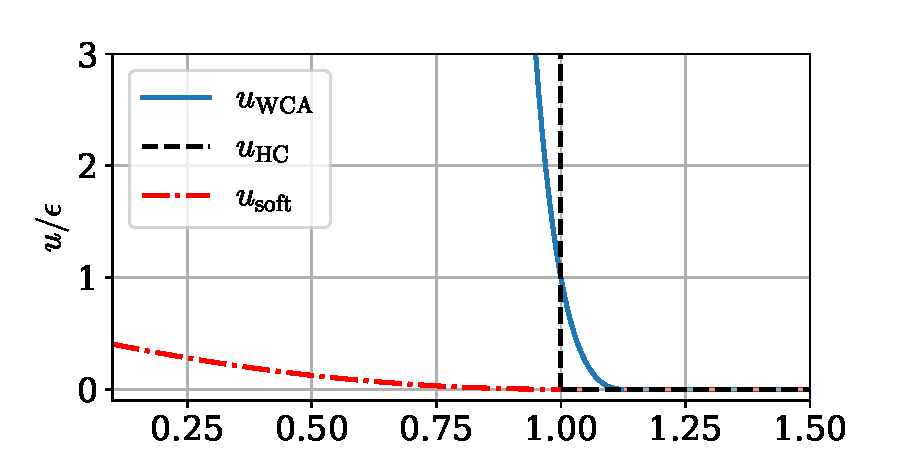
\includegraphics[width=.4\textwidth]{chapters/Figures/scalar/pot.pdf}
    \caption{Illustration of the possible choices for the potential $u$. A hard repulsion corresponds to $\lim_{r\to0} u(r) = +\infty$, such that the particles can never fully overlap. On the other hand, for the soft repulsion the maximum value of the potential is finite, such that overlaps are always possible.}
    \label{fig: hard soft}
\end{figure}


In \autoref{chapter: introduction}, we wrote down the Fokker-Planck equation for the single particle, \autoref{eq_FP_BM}, which describes the time evolution of the probability distribution of the system, $\calP(\bm x, t) = \E{\delta(\bm r(t) - x)}$.
We can likewise write the Fokker-Planck for a single active Brownian particle, whose probability-density also depends on the angle of said particle
%
\begin{align}
    \calP(\bm x, \phi, t)
    =
    \E{\delta(\bm x - \bm r(t))\delta(\phi - \theta(t))}.
\end{align}
%
This obeys the Fokker-Planck equation
%
\begin{align}
    \partial_t \calP(\bm x, \phi, t)
    + \bm \nabla \cdot [
        v_0 \hat {\bm e}(\phi ) \calP(\bm r, \phi, t)
        - D \bm \nabla \calP(\bm x, \phi, t)
    ]
        - D_r \partial_\phi^2 \calP(\bm x, \phi, t)
        = 0,
\end{align}
%
which describes how the probability distribution of a single ABP, or equivalently density of a large number of non-interacting ABPs, evolves with time.

When we consider $N$ \emph{interacting} particles, however, the picture becomes significantly more complicated.
We now have to consider the $N$-body distribution,
%
\begin{align}
    \calP_N(\{\bm x_i, \phi_i\}, t) = \E{ \prod_i \delta(\bm r_i(t) - \bm x_i)\delta(\theta_i(t) - \phi_i) },
\end{align}
%
and its corresponding Fokker-Planck.
If the particles are non-interacting, the probability distribution simply factors into $N$ independent one-body distributions, while interactions introduce non-trivial correlations.
One way of tackling this is the Bogoliubov-Born-Green-Kirkwood-Yvon (BBGKY) hierarchy, which is described in \autoref{appendxi: BBKGY}.
We will instead make a simplifying mean-field assumption about the effects of the interaction.

Consider a single particle moving freely, far from any other particles.
This will move at a velocity close to the self-propulsion velocity.
If, instead, the particle is in an area with a high density, the other particles will act as barriers due to their repulsive interactions, slowing our particle down.
As an analogy, imagine the difference between running in an open feel versus trying to move in a crowd at a concert.
With this picture in mind, we assume that the effective self-propulsion speed will be lowered as the local density of particles increases, and replace the constant self-propulsion speed with one that depends on the density $\rho$,
%
\begin{align}
    v_0 &\rightarrow v(\rho), &
    \odv{v}{\rho} & < 0,
\end{align}
%
and neglect any other effects of the interaction between the particles.
In general, we may consider a self-propulsion speed dependent on space and time, $v = v(\bm x, t)$.
The case above is then a special case where the temporal and spatial dependence of $V$ is through $\rho(\bm x, t)$.
The Fokker-Planck equation for the one-particle density is then
%
\begin{align} \label{eq: space dependent fokker planck}
    \partial_t \calP(\bm x, \phi, t)
    + \bm \nabla \cdot [
        v(\bm x, t) \hat {\bm e}(\phi ) \calP(\bm x, \phi, t)
        - D \bm \nabla \calP(\bm x, \phi, t)
    ]
        - D_r \partial_\phi^2 \calP(\bm x, \phi, t)
        = 0,
\end{align}
%
This equation has no simple analytical solution.
However, in the regime where $t\gg 1 / D_R \equiv \tau_R$ it may be described well using \emph{moment expansion}.
This is a powerful technique is is also very useful for more complex situations.



\subsection{Spatial variation}

If the environment of the Active Brownian particles, such as the surface they move in, varies as a function of space, then we expect the self-propulsion velocity to do so as well.
Before we start with the momentum expansion, we consider the case where the local velocity depends on space directly, not through the density of particles.
This can be achieved experimentally by engineering the environment of active particles, which leads to rich behavior, and this is described by \autoref{eq: space dependent fokker planck}.\todo{add sources, discuss more?}
We will consider only the stationary state solution, $\calP_{SS}$, which by assumption obeys $\partial_t \calP_{SS}{\bm x, \phi, t} = 0$.
We assume this state to be isotropic, $\partial_\phi \calP(\bm x, \phi, t) = 0$, so probability density is proportional to the particle density, $\rho_{SS} \propto \calP_{SS}$, and that the diffusion $D$ is small compared to the active velocity, so this term can be neglected.
From \autoref{eq: space dependent fokker planck}, the equation for the steady state then beomces
%
\begin{align}
    \bm \nabla \cdot [v(\bm x) \hat {\bm e}(\phi ) \rho_{SS}(\bm x)] = 0
    \implies 
    \rho_{SS}(\bm x) \propto \frac{1}{v(\bm x)}.
\end{align}
%
The particles thus clump together where the active velocity is high, leading to higher density, while in the regions with high active velocity, the density is low.

\begin{figure}[!htb]
    \centering
    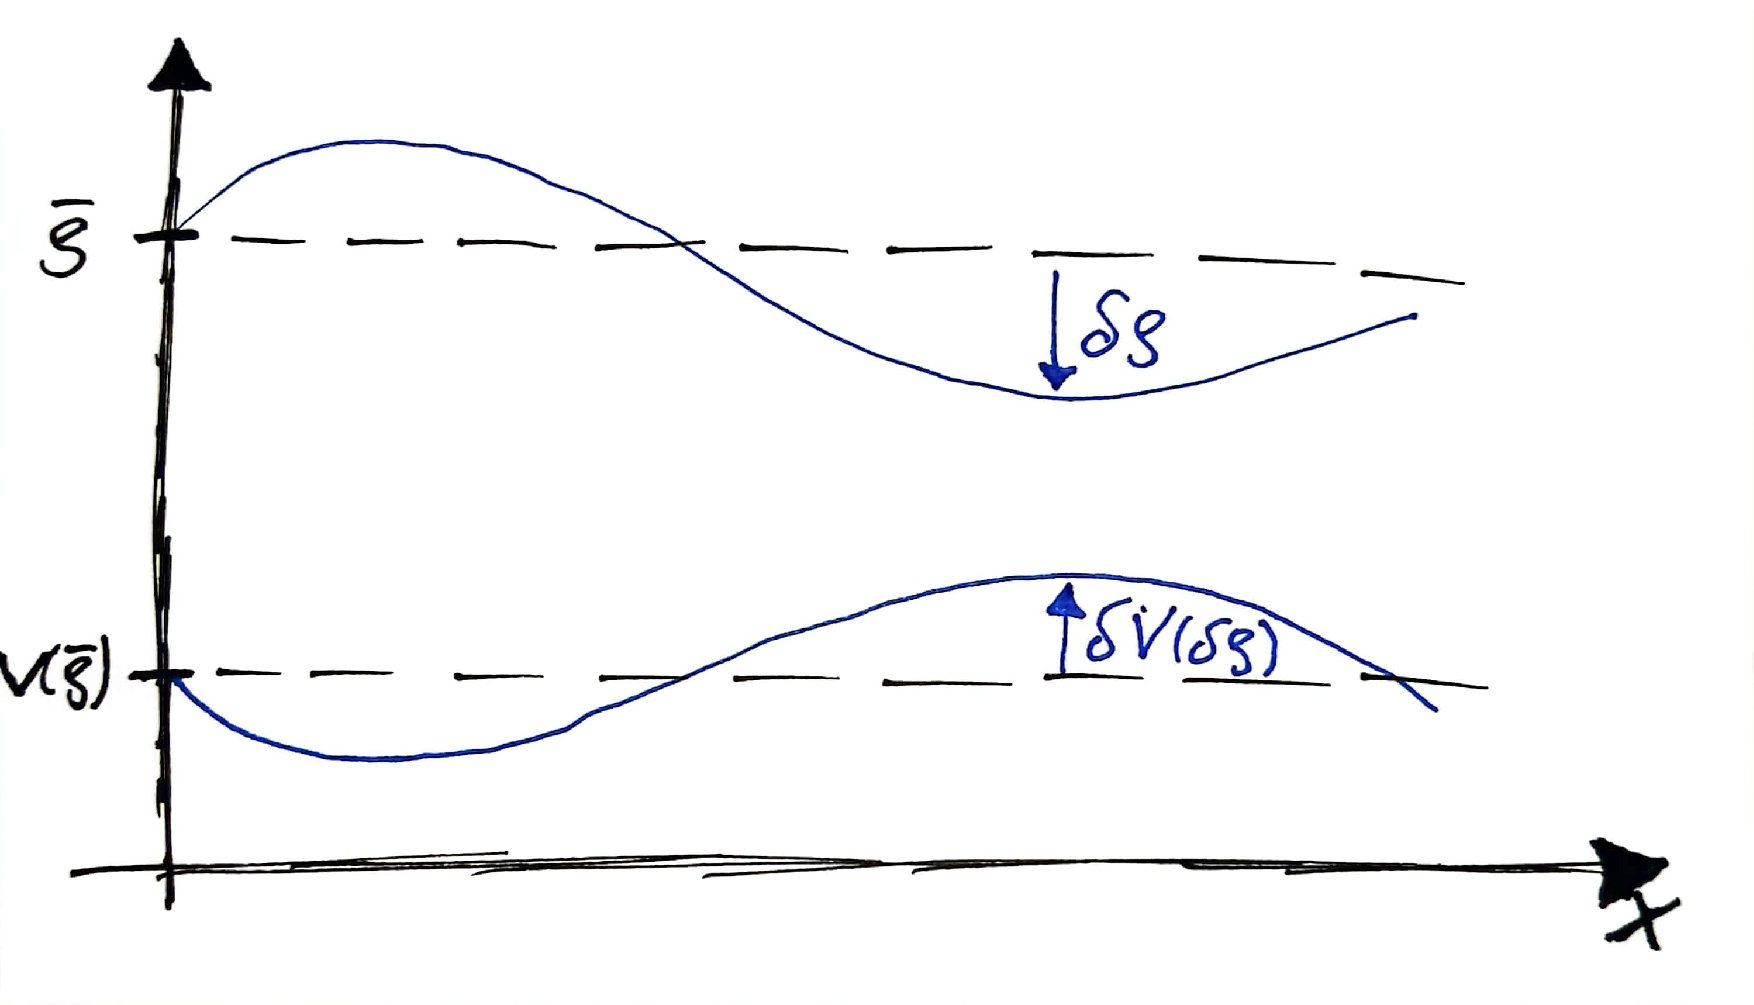
\includegraphics[width=.35\textwidth]{chapters/Figures/scalar/perturb.pdf}
    \caption{Perturbation in density gives perturbation in velocity}
    \label{fig: perturb}
\end{figure}

We now consider what happens if we pertrub a homogenous state, $\rho= \bar \rho + \delta \rho$.
Then, the velocity changes as $v(\rho) = v(\bar \rho) + \delta \rho v'(\bar \rho)$.
This will again perturb the density further, $\delta \rho'$.
Inserting this into the steady state, with $\calP = \rho$, we get
%
\begin{align}
    \bar \rho + \delta \rho'
    \propto 
    \frac{1}{v(\bar \rho) + \delta \rho v'(\bar \rho)}
    \sim \frac{1}{v(\bar \rho)} \left( 1 - \frac{\delta \rho v'(\bar \rho)}{v(\bar \rho)} \right)
    =
    \rho\left( 1 - \frac{\delta \rho v'(\bar \rho)}{v(\bar \rho)} \right)
    .
\end{align}
%
This gives a criterion for whether the perturbations are growing in strength or diminishing in strength.
If $\delta \rho' > \delta \rho$, the system is unstable.
This happens if
%
\begin{align}
    \frac{\bar \rho v'(\bar \rho)}{v(\rho)} < -1.
\end{align}
%




\subsection{Moment expansion}

To find the full dynamics of the particle density
%
\begin{align} \label{scalar order parameter}
    \rho(\bm x, t) = \int\limits _0^{2\pi} \dd \phi\, \calP(\bm x, \phi, t),
\end{align}
%
we must apply the \emph{moment expansion}.
We will see that the dynamics of $\rho$, which is the first moment of the probability distribution $\calP(\phi)$, will depend on the higher moments, of the distribution.
This creates a hierarchy of equations, which we will argue can be truncated, yielding a closed set of equations.
In addition to the particle density~\autoref{scalar order parameter}, also called the scalar order parameter, the relevant moments are the polar and nematic order fields,
%
\begin{align}
    \label{polar order parameter}
    \rho(\bm x, t) p_i(\bm x, t)
    & =
    \int\limits_0^{2\pi} \dd \phi \, \hat {e}_i(\phi) \calP(\bm x, \phi, t),
    \\\label{nematic order parameter}
    \rho(\bm x, t) Q_{ij}(\bm x, t)
    & = \int\limits_0^{2 \pi} \dd \phi
    \left[
        \hat e_i(\phi)\hat e_j(\phi) - \frac{1}{2} \delta_{ij}
    \right] \calP(\bm r, \phi, t).
\end{align}
%
The polar order parameter, $p_i$, measures how much the particles align in the same direction.
If the distribution of particles is independent of the direction $\phi$, then using the explicit form of $\hat {\bm e}$~\autoref{unit vector}, we see that the polar order parameter vanishes: $\bm p = \frac{1}{2\pi} \int_0^{2\pi}\hat {\bm e}(\phi) = \bm 0$.
If the distribution is strongly peaked around som angle $\theta$, so we can approximate $\calP(\bm x, \phi, t) \propto \delta(\phi - \theta)$, then $\bm p = \hat{\bm e}(\theta)$.
In general, the polar order parameter will take on values between these extremes, varying as a function of space and time.

While the polar order parameter $\bm p$ measures the alignment of small arrows, we can consider the nematic order parameter $Q$ measures the alignment of objects that are symmetric back to front, such as an ellipse.
If the system is completely disordered, then $Q = 0$.
If 50\% of the particles points in direction $\theta = 0$, while the rest points in the opposite direction $\theta = \pi$, the $p_i = 0$, while $Q\neq 0$.
In fact, 
%
\begin{equation}
    Q = 
    \begin{pmatrix}
        1 & 0 \\ 0 & -1
    \end{pmatrix}.
\end{equation}
%
We see that $\mathrm{Tr} Q = 0$.
This is in general true for $Q$, and is due to the Krönkecker delta in its definition.
General, higher-order moments describe the alignment of objects invariant under shorter and shorter rotations.
The polar order parameter is invariant under a $2 \pi$ rotation, the nematic under a $\pi$ rotation, and so on.\footnote{
    In quantum mechanics, we must also include fields that pick up a minus sign under rotations by $2 \pi / n$.
    These are fermionic fields, while the fields introduced here are boson fields.
}
The difference between polar and nematic ordering is shown in \autoref{fig: polar and nematic}

\begin{figure}[!htb]
    \centering
    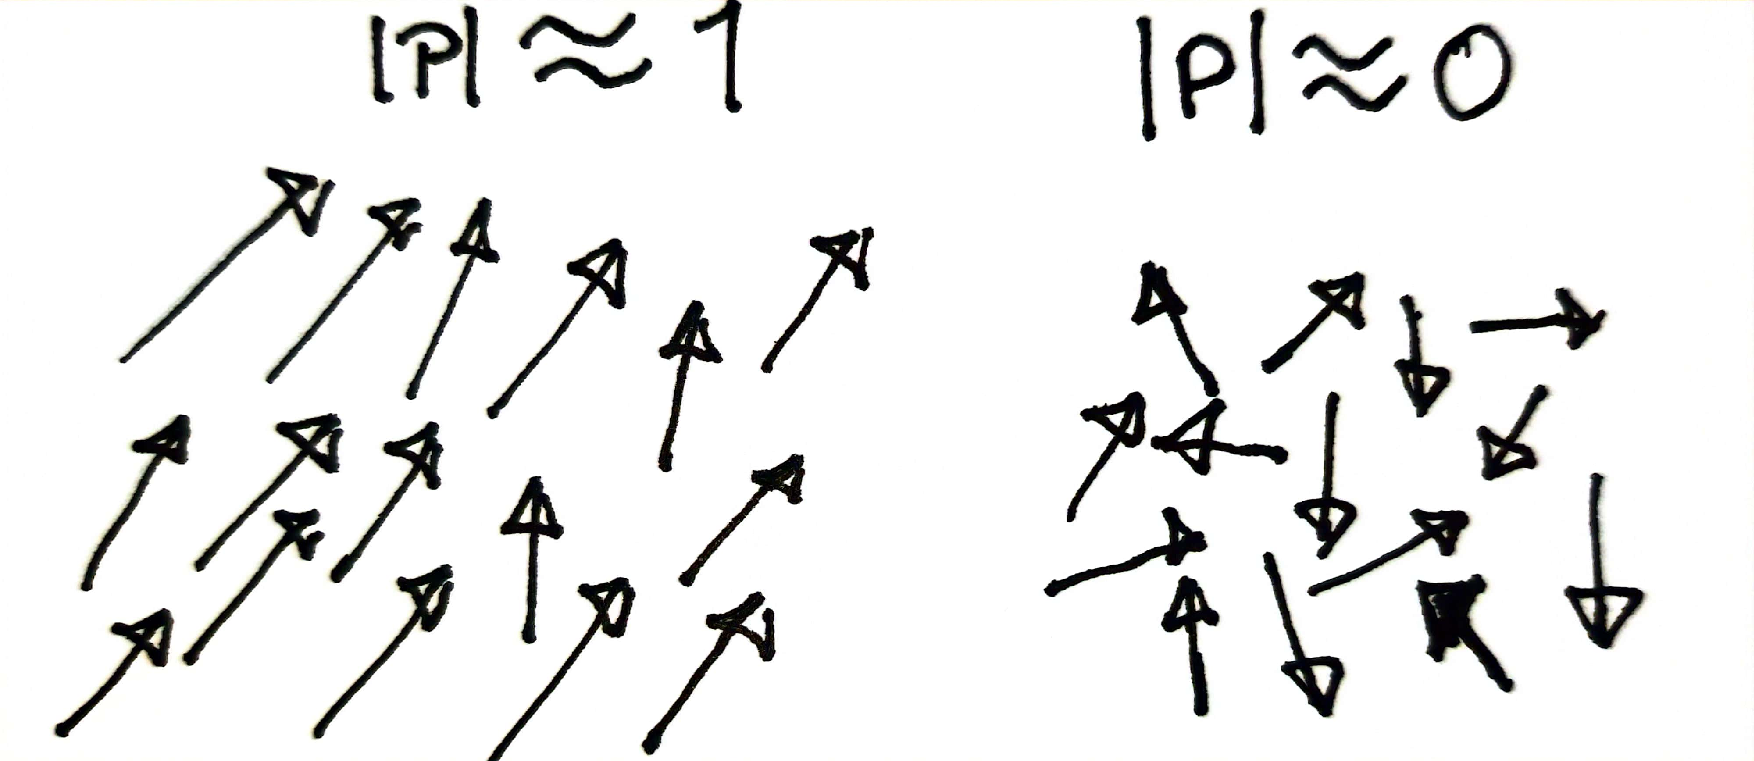
\includegraphics[width=.38\textwidth]{chapters/Figures/scalar/polar.pdf}
    \hspace{1cm}
    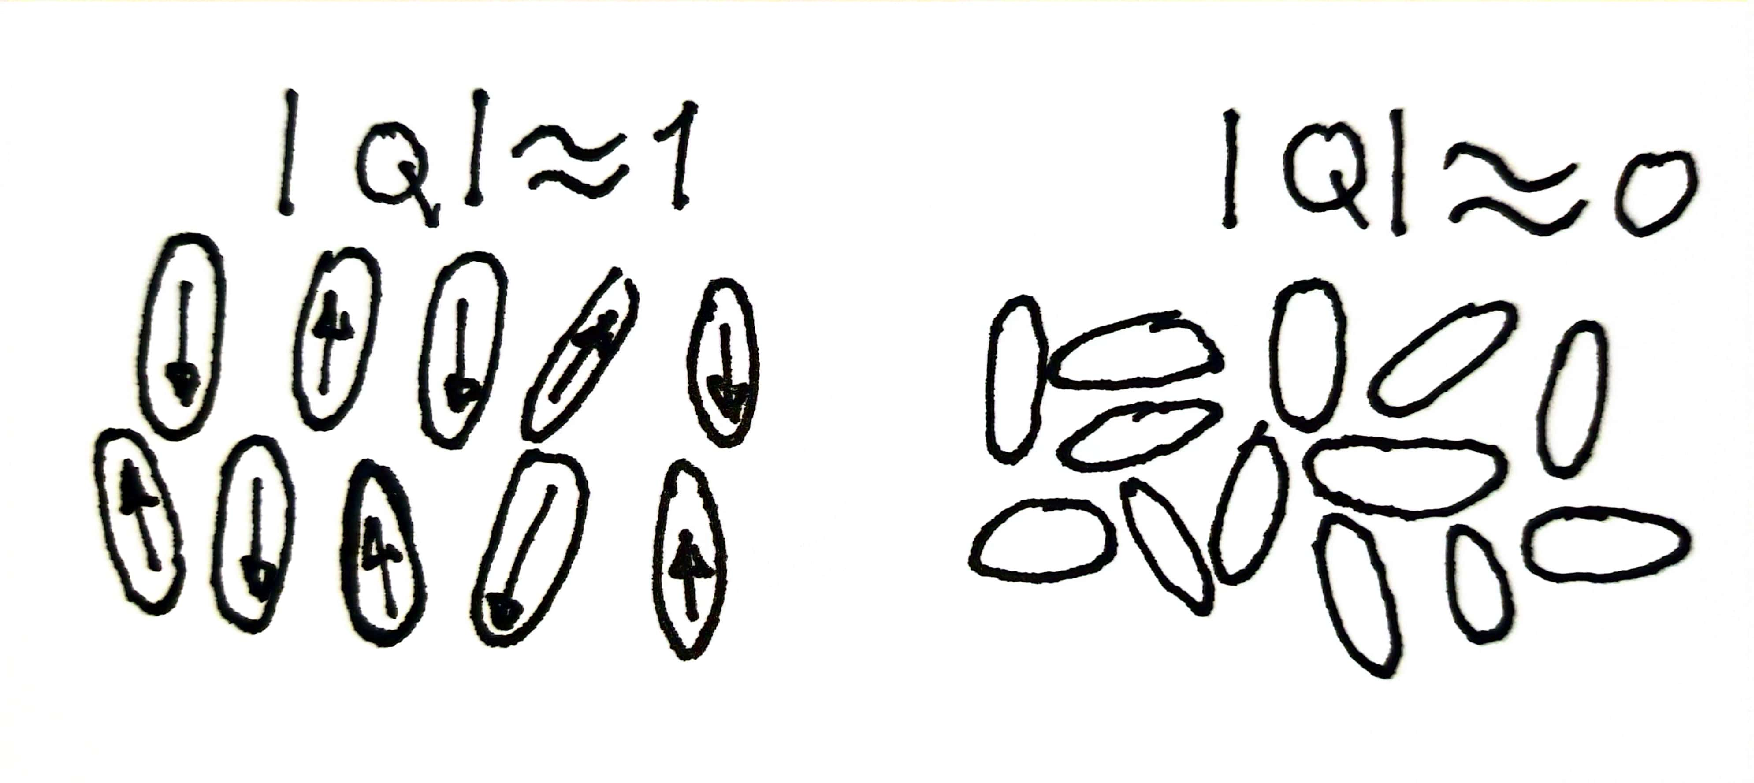
\includegraphics[width=.4\textwidth]{chapters/Figures/scalar/nematic.pdf}
    \caption{
        To the left, to configurations that have high and low polar ordering.
    To the right, two configurations which both have low polar ordering, but one has high nematic ordering, while the other has low.}
    \label{fig: polar and nematic}
\end{figure}

To derive the equations of motion of the scalar order parameter, we integrating the Fokker-Planck for the one-particle distribution over $\phi$.
In other words, we apply $\int \dd \phi$ to \autoref{eq: space dependent fokker planck}, which gives
%
\begin{align}\label{eq: density FP}
    \partial_t \rho(\bm x, t)
    = 
    - \bm \nabla \cdot [ v(\bm x, t) \rho(\bm x, t) \bm p(\bm x, t) - D \nabla \rho(\bm x, t)].
\end{align}
%
The radial diffusion term $\propto D_r$ vanishes as it is a total derivative.

% Handwritten page XI

In the same manner, we find the equation of motion for $\bm p$ by applying $\int \dd\phi \, \hat{\bm e}(\phi)$ to \autoref{eq: space dependent fokker planck}, which yields\todo[noinline]{check indices}
%
\begin{align} \label{eq: polarity FP}
    \partial_t [\rho(\bm x, t)  p_i(\bm x, t)]
    =
    -
    \nabla_{j}
    \left\{
        v(\bm x, t) \rho(\bm x, t) \left[ Q_{ij}(\bm x, t) + \frac{ 1 }{ 2 }  \delta_{ij}\right]
        - D \nabla_j [\rho p_i(\bm x, t)]
    \right\}
    - D_r \rho p_i(\bm x, t).
\end{align}
%
The last term is obtained by integration by parts.
In this equation, we are using the Einstein summation convention, which means that repeated indices are summed over.

{\it Exercise: Explain why the matrix $\bm Q$ is defined as traceless (${\sum}_i Q_{ii} = 0$). Hint: Try to calculate its expression assuming a uniform distribution of orientations.}

As we can see, this expansion is a runaway process, and we need a criterion for closing this hierarchy of equations.
When we do coarse-graining, we are interested in the large-scale, long-term behavior of the system.
We therefore remove terms that are fourth order or more in gradients.
For example, the lowest order contribution to $\partial_t \rho $ is the diffusion term, so $\rho = \Oh(\nabla^2)$.
If we were to write out the equation for the nematic tensor, we would see that $Q = \Oh(\nabla)$, so $\nabla [v \rho Q] = \Oh(\nabla^4)$ and is therefore neglected.
This closes the hierarchy of equations, and we are left with
%
\begin{subequations}
\begin{align}
    \label{eq: closed density}
    \partial_t \rho(\bm x, t) &= - \nabla_i [v(\bm x, t) p_i(\bm x, t) \rho(\bm x, t) - D \nabla_i \rho(\bm x, t)], \\
    \label{eq: closed polarity}
    \partial_t [\rho(\bm x, t) p_i(\bm x, t)]
    & = 
    - \nabla_j \left[\frac{1}{2} v(\bm x, t) \rho(\bm x, t) \delta_{ij} - D\nabla_j [\rho(\bm x, t) p_i(\bm x, t)]\right] - D_r \rho(\bm x, t) p_i(\bm x, t).
\end{align}
\end{subequations}
%
As all terms in the density equation are proportional to at least one gradient term, the only time scale in this equation in this equation is the system size, $\partial_t^{-1} \sim \nabla^{-1} \sim L$, which diverges in the thermodynamic limit $L\rightarrow\infty$.
We therefore expect this dynamics to be slow.
The equation for the polar order parameter $p_i$, on the other hand, has a time scale inherited from the rotational diffusion, $\tau_r = 1 / D_r$.
In this case, we expect any non-zero polar order to relax on a time-scale $\tau_r$, which given a large enough system will be much smaller than the time scale for the density field, leading to a \emph{separation of time scales}.
\todo[inline]{This can probably be written better\dots}

To see this, consider an equation of the form
%
\begin{align} \label{eq: enslave}
    \partial_t \rho \bm p = - D_r \rho \bm p + A(\bm r, t),
\end{align}
%
we may solve it exactly as
%
\begin{align}
    \rho(\bm x, t) \bm p(\bm x,t)
    = e^{- t D_r} \left[ \rho(\bm x, 0) \bm p(\bm x,0) + \int_0^t \dd t' \, e^{- t D_r} A(\bm x,t') \right].
\end{align}
%
We will assume now that $t\gg \tau_R$, so that the first term is suppressed, and change variables to $\tau = t - t'$, which yields
%
\begin{align}
    \rho(\bm r, t) \bm p(\bm x, t)
    & = \int_0^t \dd \tau \, e^{- \tau  D_r} A(\bm x,t - \tau)\\
    & \approx
    \int_0^\infty \dd \tau \, e^{- \tau  D_r} [A(\bm x,t ) + \tau \partial_\tau A(\bm x, t) + ...]
    \approx \frac{1}{D_r} A(\bm x, t),
\end{align}
%
where we in the last step we assume $A$ does not vary much over the time-scale $\tau_R = 1 / D_R$.
This shows that, given our assumptions, we may neglect the time-derivative term in the original equation \autoref{eq: enslave}, and dynamics of $\bm p$ is now complete determined by $A(\bm x, t)$.
We say $\bm p$ is \emph{enslaved} to the slow dynamics of $A$.
Finally, we see that the diffusion term, proportional to $D$ in \autoref{eq: closed polarity}, is fourth order in gradients, and should therefore be neglected.\todo[noinline]{Is this counting right?}

We now return to the special case of a density-dependent self-propulsion velocity, $v(\bm x, t) = v(\rho(\bm x, t))$.
We can now explicitly solve for the polar order,
%
\begin{align}
    \rho p_i = 
    - \frac{1}{2 D_r} \nabla_i  [v(\rho) \rho].
\end{align}
%

A sanity check is to now substitute back in the special case $v(\rho) = v_0$, corresponding to non-interacting ABPs.
The polar order-parameter is then given by
%
\begin{align}
    \rho \bm p = - \frac{v_0}{2 D_R} \bm \nabla \rho,
\end{align}
%
which when substituted back into Fokker-Planck for the density, \autoref{eq: density FP}, gives
%
\begin{align}
    \partial_t \rho &= D_{\mathrm{eff}} \nabla^2 \rho, &
    D_{\mathrm{eff}} = D + \frac{v_0^2}{2 D_R},
\end{align}
%
which is excatly what we found in \autoref{chapter: introduction}.

% Handwritten XII

\textit{{\bf Homework}:
In two dimensions, the vector $\he(\theta) = (\cos\theta, \sin\theta)$ is parametrized by the angle $\theta_t$. Assuming that $\theta_t$ is a Markov process, justify why we can write the joint distribution as $P(\theta_2,t_2;\theta_1,t_1) = P(\theta_2-\theta_1,t_2-t_1|0,0)P(\theta_1,t_1)$ for $t_2 > t_1$.
Deduce that
\begin{equation*}
    \langle \he(\theta_t) \cdot \he(\theta_{t+\tau}) \rangle = \int \rmd\phi \cos\phi \, P(\phi,\tau|0,0) \equiv \langle \cos\phi \rangle_0, 
\end{equation*}
where $P(\theta,t)$ is the distribution of $\theta$ satisfying $P(\theta,0) = \delta(\theta)$.
(Hint: Use the properties of $\theta$ to express the joint distribution $P(\theta_2,t_2;\theta_1,t_1)$)
}



\subsection{MIPS}

If we take the more general case, where the active velocity depends on the density, $|v_a| = v(\rho)$, we may write the Fokker-Planck for the density as a conservation law
%
\begin{align}
    \partial_t \rho(\bm x, t)  = - \bm \nabla \cdot \bm J(\bm x, t),
\end{align}
%
where the current has the form \todo[noinline]{Is the factor $\rho$ right?}
% 
\begin{align}
    J[\rho] = - \rho M[\rho] \bm \mu[\rho].
\end{align}
%
Here, we have introduced the mobility,
%
\begin{align}
    M[\rho] = \frac{v[\rho]^2}{2 D_r},
\end{align}
%
and the chemical potential
%
\begin{align}
    \mu[\rho] = \ln(\rho v[\rho]).
\end{align}
%
This chemical may be written as the derivative of a free energy,
%
\begin{align}
    \mu(\rho) = f'(\rho) \implies
    f(\rho) = \int^\rho \dd x \, \ln (v[x] x).
\end{align}
%
This means that we can apply the methods of equilibrium theory of phase separation.
This is detailed in \autoref{chapter: phase sep}.
If we assume there is a homogenous solution $\rho = \bar \rho$, this will be unstable if $f''(\bar \rho) < 0$.
Inserting this into the free energy we found, we get the criterion
%
\begin{align}
    \frac{v'(\bar \rho)\bar \rho}{v(\bar \rho)} < - 1.
\end{align}
%
This gives the \emph{spinodals}, where the system is unstable for any perturbation.
However, as described in \autoref{chapter: phase sep}, the new phases are described by the \emph{binodals}.
Following the procedure laid out there, we write the equations for chemical and mechanical equilibrium for the two phases with density $\bar \rho_i$ and volume $\V_i$,
%
\begin{align}
    \V_i[f'(\bar \rho_i) - \mu] &= 0, \\
    f(\bar \rho_i) - \mu \rho_i + P &= 0,
\end{align}
%
whose solution gives the volumes and density of each phase given an overall density $\bar \rho$.

This is called motility-induced phase-separation, as the mechanism of phase is not attraction, as in passive systems, but a lowering of the motility in high densities.
The mechanics of phase separation are thus non-equilibrium, however, the resulting large-scale dynamics are still described by an effective equilibrium theory.
This comes as we can always find free energy, no matter the shape of $v(\rho)$.
To break equilibrium also at the large scale, we must have a more general current.
One way to obtain this is to extend the momentum expansion to higher orders.


\section{Top-down approach}

\subsection{Active model B}

Another way to achieve a model with out-of-equilibrium effects is to take the Ginzbur-Landau approach and write down all possible terms allowed by symmetry and conservation.
We begin with the conservation law,
%
\begin{align}
    \partial_t \rho = - \bm \nabla \cdot \bm J,
\end{align}
%
and write the current as
%
\begin{align}
    \bm J = 
    - \rho M(\rho) \bm \nabla 
    \left[
        f'(\rho) - K \nabla^2 \rho + \lambda |\nabla \rho|^2
    \right]
    + \zeta \nabla^2 \rho \bm \nabla \rho.
\end{align}
%
The two first terms may be written in terms of a free energy functional.
The two next cannot, due to the gradient structure.
With only the $\lambda$ term, this is called the active model B.
It was later discovered that another term was possible to include, namely the $\zeta$ term.
With this addition, the model is called active model B+.
More details on this model are given in \autoref{section: active model B top down}.






\section{Scalar active matter: a bottom-up approach}



\subsection{Motility Induced Phase Separation}

\todo[inline]{Should this be included?}

We now use the fact that the spatial dependencies of $v$ and $D$ come from their dependencies in the local density field $\phi$. We thus consider
\begin{equation} \label{eq_local_coeffs}
    v(\bm r) = v(\phi(\bm r)), \qquad D(\bm r) = D(\phi(\bm r)).
\end{equation}
Now Equation~\eqref{eq_closed_phi} for the particle density takes the form of simple diffusion equation $\partial_t\phi = \nabla \cdot [D_{\rm eff}(\phi)\nabla\phi]$ with effective nonlinear diffusivity
\begin{equation} \label{eq_Deff_QS}
    D_{\rm eff}(\phi) = D(\phi) + \frac{v^2(\phi) + \phi v'(\phi) v(\phi)}{d (d-1) D_r} ,
\end{equation}
where as previously primes denote derivatives wrt $\phi$.
As we immediately note, if the effective self propulsion speed $v(\phi)$ of the active particles decreases fast enough when their local density increases, $D_{\rm eff}(\phi)$ may become negative leading to, as we discussed in Sec.~\ref{sec_top_down}, spinodal decomposition of a state with uniform density $\bphi$. Namely, the corresponding condition reads
\begin{equation} \label{eq_cond_MIPS_sp}
    1 + \frac{\bphi v'(\bphi)}{v(\bphi)} < -\frac{d (d-1) D_r D(\bphi)}{v^2(\bphi)} .
\end{equation}
As we discussed previously, this instability will lead to a phase separated state between a dense, slow liquid and a dilute, fast gas. Remarkably, this phase separation phenomenon occurs despite the absence of explicit attractive interactions between the particles, but is induced by a nonequilibrium characteristic which couples the particle local density to their self propulsion force.
Namely, if active particles accumulate in regions of low self propulsion speeds while the latter decreases with the local density, a positive feedback loop sets in leading small density perturbations to be naturally amplified.
This phenomenon is known as \emph{Motility Induced Phase Separation (MIPS)}~\cite{CatesMIPS}.
Neglecting positional diffusion, the condition~\eqref{eq_cond_MIPS_sp} simplifies as $v'(\bphi)/v(\bphi) < -1/\bphi$.

Eq.~\eqref{eq_cond_MIPS_sp} defines the spinodals of MIPS.
As we saw in Sec.~\ref{sec_top_down}, calculating the corresponding binodals then imposes to know which nonlocal (higher order in gradients) terms will appear in the dynamics of $\phi$. 
At the level of Eq.~\eqref{eq_local_coeffs} this can be done by relaxing the constraint that the effective self-propulsion speed and diffusivity depend on locally on the density field. Considering, on the contrary, a short ranged interaction kernel $K(|\bm r|)$ such that
\begin{equation}
    v[\phi] = \tilde{v}\left(\intd{r'} K(|\bm r - \bm r'|)\phi(\bm r') \right),
    \qquad D[\phi] = \tilde D\left(\intd{r'} K(|\bm r - \bm r'|)\phi(\bm r')\right),
\end{equation}
we can expand $\tilde v$ and $\tilde D$ in the gradients of $\phi$ which leads to
\begin{equation} \label{eq_nonloc_coeffs}
    v[\phi] \simeq \tilde v(\phi) + \frac{\ell^2}{2}\tilde v'(\phi) \nabla^2\phi ,
    \qquad
    D[\phi] \simeq \tilde D(\phi) + \frac{\ell^2}{2}\tilde D'(\phi) \nabla^2\phi ,
\end{equation}
where we have used the fact that $K$ is isotropic and normalized to unity, while 
$\ell^2 \equiv \intd{r} K(|\bm r|) |\bm r|^2$.

\paragraph{Absence of positional diffusion}
In the case where $D[\phi]$ can be neglected, Eq.~\eqref{eq_closed_phi} takes the form
\begin{equation} \label{eq_phi_AMB_mapping}
    \partial_t\phi = -\nabla\cdot \bm J, \qquad \bm J = -M_{\rm eff}[\phi]\phi \nabla \ln(v[\phi]\phi),
\end{equation}
where the effective mobility is defined as $M_{\rm eff}[\phi] = v^2[\phi]/(d(d-1)D_r)$. Using the nonlocal expression of the self propulsion speed~\eqref{eq_nonloc_coeffs}, we find that the model maps onto AMB with the effective chemical potential given by
\begin{equation}
    \mu = \ln(\tilde v(\phi) \phi) - \kappa(\phi)\nabla^2 \phi, \qquad \kappa(\phi) = -\frac{\ell^2}{2}\frac{\tilde v'(\phi)}{\tilde v(\phi)}.
\end{equation}
In this case the binodals can thus be calculated from the free energy mapping that we studied in Sec.~\ref{sec_top_down}~\cite{Solon2018}.

\paragraph{The case with positional diffusion}
If $D[\phi]$ cannot be neglected, on the contrary, then one can easily check that the current in Eq.~\eqref{eq_phi_AMB_mapping} includes terms of the form $\sim (\nabla^2\phi)\nabla\phi$ which cannot be written as deriving from a generalized chemical potential. This case corresponds to the AMB+ (active model B+) class which, as shown in Ref.~\cite{Tjhung2018PRX}, shows a qualitatively different physics than that of AMB or equilibrium phase separation.
Indeed, such non-curl free current is responsible for the emergence reversed Ostwald ripening selecting a preferred (finite) phase separated domain length scale.
Although a comprehensive derivation of such term from coarse-graining approaches at outlined in this section is still missing, such microphase separation scenario has recently been shown to be revelant in numerical simulations of microscopic models of ABPs with pairwise repulsion~\cite{Caporusso2020MIPS,Shi2020bubbles}. 




    \chapter{The Non-Reciprocal Cahn-Hilliard model - Lecture 6}
    \label{chap_nrch}
    \section{Introduction}
Continuing with last few lectures where active phase separation was discussed, today I will introduce yet another model describing pattern formation out of equilibrium. I will introduce and discuss properties what we call - the non-reciprocal Cahn-Hilliard model. The dynamics of two passive colloidal particles interacting in a fluid medium is 
\beq
m \frac{d^2 \br_1}{dt^2} + \Gamma_1 \frac{d \br_1}{dt} &=& \bm{F}(\br_2 - \br_1) \\ \nonumber
m \frac{d^2 \br_2}{dt^2} + \Gamma_2 \frac{d \br_2}{dt} &=& \bm{F}(\br_1 - \br_2).
\label{eq:EqDynamics}
\eeq
Action reaction symmetry is 
\beq 
\bm{F}(\br_1 - \br_2) = - \bm{F}(\br_2 - \br_1)
\eeq 
This is explicitly not true for symmetric colloids which responds to chemical gradients produced by one another. The model we will describe today describes the dynamics of a collection of such colloids when the interactions are short ranged.  

\section{Multicomponent phase separation}
Consider for simplicity two conserved density fields $\phi_1$ and $\phi_2$ corresponding to the number concentrations of two chemical species $1$ and $2$ respectively. Assume that the system at constant volume $V$ fractionates into two phases with volumes $V_1$, $V_2$ and compositions $\phi_1^{(1)}, \phi_2^{(1)}$ in phase 1 and $\phi_1^{(2)},\phi_2^{(2)}$ in the two phases. Our objective is obtain conditions for phase equilibrium. Volume and number conservation constrains these quantities as 
\begin{eqnarray}
    V_1 +V_2 &=& V  \\
     \phi_1^{(1)} V_1 + \phi_1^{(2)} V_2 &=&  \bar{\phi_1} V \\
     \phi_2^{(1)} V_1 + \phi_2^{(2)} V_2 &=&  \bar{\phi_2} V.
     \label{eq:constraints}
\end{eqnarray}
The free energy of the homogeneous system is $\mathcal{F}(N_1,N_2,V,T)$. For constant temperature $T$ or any other external control parameter like Ph and noting that the free energy is extensive with respect to volume, the total free energy receives contribution from the two phases 
\begin{eqnarray}
\mathcal{F} = V_1 f(\phi_1^{(1)},\phi_2^{(1)}) + V_2 f(\phi_1^{(2)},\phi_2^{(2)}).
\label{eq:TotalFreeEnergy}
\end{eqnarray}
The unconstrained free energy $\bar{\mathcal{F}}$ is obtained by introducing Lagrange multipliers $P$ conjugate to the total volume and $\mu_1,\mu_2$ conjugate to the two conserved fields - 
\begin{eqnarray}
\bar{\mathcal{F}} = \mathcal{F} +P(V_1 + V_2) - \mu_1 (V_1 \phi_1^{(1)} + V_2 \phi_2^{(1)}) - \mu_2 (V_1 \phi_2^1 + V_2 \phi_2^2).
\end{eqnarray}
Minimizing $\bar{\mathcal{F}}$ with respect to the six unknown quantities, we find three more conditions for phase equilibrium
\begin{eqnarray}
\mu_1 &=& \frac{\partial f(\phi_1^{(1)},\phi_2^{(1)})}{\partial \phi_1^{(1)}} = \frac{\partial f(\phi_1^{(2)},\phi_2^{(2)})}{\partial \phi_1^{(2)}}. \\
\mu_2 &=& \frac{\partial f(\phi_1^{(1)},\phi_2^{(1)})}{\partial \phi_1^{(1)}} = \frac{\partial f(\phi_1^{(2)},\phi_2^{(2)})}{\partial \phi_1^{(2)}}. \\
P &=& -f + \mu_1 \phi_1^1 + \mu_2 \phi_2^1  = -f + \mu_1 \phi_1^2 + \mu_2 \phi_2^2. 
\label{eq:Equilibrium}
\end{eqnarray}
Eqs. \eqref{eq:constraints} and \eqref{eq:Equilibrium} can be solved to obtain the Binodals. These equations represent a generalisation of the Maxwell construction for N=1. Similar equations can be written and solved for N components and $n$ phases. Gibbs phase rule relates the number of free parameters that can be tuned, F, to the number of components $C$, number of phases $P$ as $F = C-P+2$. Going back to $N=2$, Figure \ref{fig:BinaryPD} shows the variety of phase diagrams and critical points that are possible. 

For a binary system, average compositions of the two phases are be tuning parameters. The Maxwell construction can be discussed geometrically for a single component. For a given free energy $f$, let's consider binary phase separation such the compositions are $\phi^{(1)}$ and $\phi^{(2)}$. Equality of chemical potentials and pressure is enforced by the construction of a common slope and common intercept.
\section{Phase separation - dynamics}
The relaxational dynamics of the fields $\phi_{1,2}$ are given by a generalisation of the Cahn-Hilliard dynamics. 
\begin{eqnarray}
\partial_t \phi_i(\bm{r},t) + \bm{\nabla} \cdot \bm{J}_i &=& 0 \\
 \bm{J}_i &=& - \bm{\nabla} \mu_{i}^\mathrm{eq}   +  \bm{\zeta}_i,
\end{eqnarray}
We choose a general form for $f  = f_1(\phi_1) + f_2(\phi_2) + f_{I}(\phi_1,\phi_2)$. A simple choice, often made for the Flory-Huggins system is $f_I = \chi \phi_1 \phi_2$, contributes , linear terms to $\mu_{1,2}$. For $\chi <0$, the densities modulations co-locate simulating attractive microscopic interactions while $\chi>0$ the densities anti-co-locate simulating repulsive microscopic interactions. 
\\
This equation describes dissipative relaxational dynamics.
\\
The bulk free energy should be supplemented by an interfacial free energy that ensures that interfaces are smooth. 
\\
The system evolves to a stationary state (time independent) state when the chemical potential $\mu$ is equal throughout the system. the steady state is uniquely determined by statics discussed in the previous section. 
\\
We choose a polynomial form for the single species free energy. 
\beq 
f(\phi_1) = (T-T_c) \frac{\phi_1^2}{2} + \frac{\phi_1^4}{4}
\eeq
Let us sketch the form of $f$, it has distinct forms for $T<T_c$ and for $T>T_c$. What does the phase diagram look like in the $T -- <\phi>$ plane? Discuss the critical point and the first order lines of transition.

For two components we have similar diagrams in the plane of composition. 


What information can we add about the dynamics? Let's consider again a single component system and ask what happens if we start from a random initial condition and allow the system to evolve.


\section{Non-reciprocal Cahn-Hilliard Dynamics}
We will now introduce a new kind of activity in the system - non-reciprocity. We add terms to the chemical potential which cannot be derived from a free energy.  
\beq
\mu_i^{neq} = \mu_i^{eq} + \sum_j \alpha_{ij} \phi_j.
\eeq


\subsection{Non-reciprocal interactions in a binary mixture}
For a binary mixture, the free energy can be written as
\begin{eqnarray}
F &=&  \int \mathrm{d}\bm{r} \bigg\{ \sum_{i=1}^{2} (\phi_i-c_{i,1})^2(\phi_i-c_{i,2})^2  \nonumber \\ 
&& + \chi \phi_1 \phi_2 + \chi' \phi_1^2 \phi_2^2  
+ \revise{\frac{\kappa}{2}}  \sum_{i=1}^{2} |\bm{\nabla} \phi_i|^2  \bigg\},
\label{FreeEnergy2}
\end{eqnarray}
which results in the equilibrium chemical potentials
\begin{eqnarray}
\mu_1^\mathrm{eq} &=& \revise{2} (\phi_1 - c_{1,1})(\phi_1 - c_{1,2})(2\phi_1 - c_{1,1}- c_{1,2}) + \chi \phi_2 \nonumber \\
&& + 2 \chi' \phi_1 \phi_2^2, \nonumber \\
\mu_2^\mathrm{eq} &=& \revise{2} (\phi_1 - c_{2,1})(\phi_1 - c_{2,2})(2\phi_1 - c_{2,1}- c_{2,2})  + \chi \phi_1 \nonumber \\
&& + 2 \chi' \phi_2 \phi_1^2.
\label{ChemPot}
\end{eqnarray}
We note that, at equilibrium, the sign and strength of the interaction between the two components is governed by $\chi$. If $\chi>0$, the interaction between the two species is repulsive (their overlap increases the free energy of the system), whereas if $\chi<0$, the interaction is attractive (overlap decreases the free energy of the system). For two components, the activity matrix $\alpha_{ij}$ is simply given by $\alpha_{11}=\alpha_{22}=0$, and $\alpha_{12}=-\alpha_{21}=\alpha$, and there is a single scalar parameter $\alpha$ representing the non-reciprocal activity. The non-equilibrium chemical potentials become 
\begin{eqnarray}
 \mu^\mathrm{neq}_1 = \mu_1^\mathrm{eq} + \alpha \phi_2, \nonumber \\
 \mu^\mathrm{neq}_2 = \mu_2^\mathrm{eq} - \alpha \phi_1.
 \label{ChemPot2}
\end{eqnarray}

Considering the form of the equilibrium chemical potentials (\ref{ChemPot}), it becomes clear that the activity $\alpha$ acts to modify the equilibrium interaction parameter $\chi$ within the non-equilibrium chemical potential, so that we find a term $(\chi + \alpha) \phi_2$ in $\mu^\mathrm{neq}_1$, and a term $(\chi - \alpha) \phi_1$ in $\mu^\mathrm{neq}_2$. A direct numerical simulation of the NRCH equations in \eqref{eq:nrch} starting from random initial conditions shows that the time translation invariance of the bulk-phase separated state is broken when $|\alpha|>|\chi|$.


\subsection{Stability analysis of the mixed binary system}
In order to obtain more analytical insight into the nature of the instabilities in the system, we linearize the dynamics of the binary NRCH model around a homogeneous state $(\avOne, \avTwo)$ to obtain
\begin{eqnarray}
\begin{pmatrix}
	\dot{\phi_1}(\bm{q}) \\
	\dot{\phi_2}(\bm{q})
\end{pmatrix}
&=& \begin{pmatrix} \mathcal{D}_{11} & \mathcal{D}_{12} \\ \mathcal{D}_{21} & \mathcal{D}_{22} \end{pmatrix}  \begin{pmatrix}
	{\phi_1}(\bm{q}) \\
	{\phi_2}(\bm{q})
\end{pmatrix}, \label{eq:matrixeq}
\end{eqnarray}
where the components of the matrix $\mathcal{D}$ are given by
\begin{eqnarray}
\mathcal{D}_{11} &=& -q^2 [ 2 (\avOne - c_{1,1})^2 + 8 (\avOne - c_{1,1}) (\avOne - c_{1,2})  \nonumber \\ && + 2 (\avOne - c_{1,2})^2 + 2 \avTwo^2 \chi'], \nonumber \\
\mathcal{D}_{12} &=& -q^2 [ (\chi+\alpha) +  4 \avOne \avTwo \chi' ],  \nonumber \\
\mathcal{D}_{21} &=& -q^2 [ (\chi-\alpha) +  4 \avOne \avTwo \chi' ],  \nonumber \\
\mathcal{D}_{22} &=& -q^2 [ 2 (\avTwo - c_{2,1})^2 + 8 (\avTwo - c_{2,1}) (\avTwo - c_{2,2})  \nonumber \\ && + 2 (\avTwo - c_{2,2})^2 + 2 \avTwo^2 \chi'], \nonumber
\end{eqnarray}
Recall that the stability of the homogeneous state defined by uniform $\bar{\phi}_i$ is determined by the signs of the eigenvalues of the matrix \eqref{eq:matrixeq}. In the absence of activity $\alpha=0$, the matrix $\mathcal{D}_{ij}$ is symmetric and thus only admits real eigenvalues. When the non-reciprocal activity is turned on, however, $\mathcal{D}_{ij}$ is no longer symmetric and its eigenvalues may become complex, signaling the possibility of oscillations in the NRCH model.

Indeed, a non-oscillatory instability will take place when one of the eigenvalues $\lambda_{1,2}$ is real and positive, whereas an oscillatory instability is expected when $\lambda_{1,2}$ are a complex conjugate pair with positive real part. To study the phase diagrams of the system, we define $\mathcal{C}_r$ as the region of the parameter space where either $\mbox{Re}(\lambda_1)>0$ or $\mbox{Re}(\lambda_2)>0$, and $\mathcal{C}_i$ as the region where $\mbox{Im}(\lambda) \neq 0$. A non-oscillatory instability will occur in regions of $\mathcal{C}_r$ that do not intersect with $\mathcal{C}_i$, whereas the instability will be oscillatory at the intersection between $\mathcal{C}_r$ and $\mathcal{C}_i$.


\subsection{Exceptional points}
We now explore the linear stability of the system for fixed system composition $(\avOne,\avTwo)$ and varying strength of the reciprocal and non-reciprocal interactions, governed by $\chi$ and $\alpha$ respectively. To focus on a particularly simple representative case, we set $\chi' = 0$, such that the equations of motion are now invariant under the shift $\phi_1 \to \phi_1 - (c_{1,1}+c_{1,2})/2$ and $\phi_2 \to \phi_2 - (c_{2,1}+c_{2,2})/2$, and in particular on mixtures with symmetric preferred densities $c_{1,1} = -c_{1,2} = c_1$ and $c_{2,1} = -c_{2,2} = c_2$.  The elements of the dynamical matrix $\mathcal{D}$ linearized around the average composition $(\avOne,\avTwo)=(0,0)$ then become
\beq
\mathcal{D}_{11} &=&  4 q^2 c_1^2, \nonumber \\
\mathcal{D}_{12} &=&  - q^2 (\chi+\alpha), \nonumber \\
\mathcal{D}_{21} &=&  - q^2 (\chi-\alpha), \nonumber \\
\mathcal{D}_{22} &=&  4 q^2 c_2^2.
\eeq
The eigenvalues of this matrix are given by
\beq
\lambda_{1,2} = 2 q^2 (c_1^2 + c_2^2)  \pm q^2 \sqrt{(\alpha_*+\alpha)(\alpha_*-\alpha)}
\eeq
with $\alpha_* \equiv \sqrt{\chi^2 + 4(c_1^2 - c_2^2)^2}$. The corresponding (non-normalized) eigenvectors are
\beq
\eta_{1} = \begin{pmatrix}
\lambda_1 - \mathcal{D}_{22} \\
\mathcal{D}_{21}
\end{pmatrix}
~~\text{and}~~
\eta_{2} = \begin{pmatrix}
\lambda_2 - \mathcal{D}_{22} \\
\mathcal{D}_{21}
\end{pmatrix}. \label{eq:eigenvectors}
\eeq
Because the real part of $\lambda_{1,2}$ is always positive, this implies that the homogeneous state will always be unstable. This instability will become oscillatory when the two eigenvalues collide and become a complex conjugate pair, which gives the condition 
\beq
\alpha^2 \geq \alpha_*^2,
\eeq
for oscillatory behavior. Note that, at the instability, the two eigenvectors become exactly parallel to each other, as can be directly verified from (\ref{eq:eigenvectors}). The minimal value of $\alpha$ beyond which oscillations can occur is $2 |c_1^2-c_2^2|$, which occurs for $\chi = 0$, i.e. when interactions are purely non-reciprocal. The corresponding stability diagram is shown in Fig.~\ref{fig:FigChiDelta}(a), and shows two regions of oscillatory behavior at high positive and negative values of $\alpha$, separated by a gap corresponding to bulk phase separation. This gap vanishes for the singular case $c_1=c_2$, in which case the boundaries between bulk phase separation and oscillations become a pair of lines $\alpha = \pm \chi$, see Fig.~\ref{fig:FigChiDelta}(b). In the oscillatory region for positive $\alpha$, species 2 chases after species 1, whereas the opposite is true for negative $\alpha$. It is also interesting to note that oscillations can occur independently of whether the reciprocal interactions are attractive or repulsive, i.e.~independently of the sign of $\chi$. The bulk phase separated states, on the other hand, have overlapping high-density regions of both components when $\chi < 0$, and non-overlapping high-density regions for $\chi>0$.



The transition lines just described, at which two real positive eigenvalues collide to form a complex conjugate pair with positive real part and the corresponding eigenvectors become parallel, correspond to lines of what are often called \emph{exceptional points} in the non-Hermitian quantum mechanics literature \cite{Kato1995,Heiss_2012}. The coalescence of eigenvalues in this case, which implies parity-time (PT) symmetry breaking, is distinct from degeneracy of eigenlevels in Hermitian quantum mechanics where eigenvectors corresponding to degenerate levels are still non-parallel. Such exceptional points have recently been encountered in other active matter systems such as active solids with odd elasticity \cite{Scheibner2020}.




\newpage
\subsection{Oscillatory instability in the composition plane}
We now consider the phase diagrams in the average composition plane $(\avOne,\avTwo)$ for fixed $(\chi,\alpha)$. For sufficiently high values of the activity with $\alpha \gtrsim |\chi|$, we find that the spinodal splits into five disconnected regions: a middle circular part confined within $\mathcal{C}_i$ and thus corresponding an oscillatory instability, and four arms outside $\mathcal{C}_i$ extending to infinity in four directions, see Fig.~\ref{fig:Fig4}(a,b). The four arms are surrounded by the binodal region where we find bulk phase separation, see Fig.~\ref{fig:Fig4}(c). It is interesting to note that the condition $\alpha > |\chi|$ coincides with the condition required for chasing interactions between the two components to arise, i.e.~for $\chi+\alpha$ and $\chi-\alpha$ to have different sign, as described above.

In the central part of the phase diagram we find rich dynamical behavior. Let us first look at the linear stability analysis. As in the previous section, we focus again for simplicity on the special case with $\chi' = 0$, $c_{1,1} = -c_{1,2} = c_1$ and $c_{2,1} = -c_{2,2} = c_2$. In this case, the equation for $\mathcal{C}_i$ can be written as
\beq
\avOne^2 - \avTwo^2 =  \frac{1}{3} ( c_1^2 +c_2^2 - \chi^2 + \alpha^2 ),
\eeq
which defines a hyperbola,  plotted in orange in Fig.~\ref{fig:Fig4}(c). Inside this curve, where the eigenvalues are a pair of complex conjugates, the curve $\mathcal{C}_r$ is obtained by setting $\mathcal{D}_{11}+\mathcal{D}_{22} = 0$ which yields an equation for a circle with a radius independent of the  value of $\alpha$
\beq
\avOne^2 + \avTwo^2 =  \frac{1}{3}(c_1^2 + c_2^2).
\label{eqCircle}
\eeq 
At this line, which corresponds to the turquoise circle in Fig.~\ref{fig:Fig4}(c), the real part of the eigenvalues crosses from negative to positive values and the system undergoes a Hopf bifurcation, leading to oscillations.

Using simulations, we have investigated in detail the steady-state behavior in this circular region.
The phase space is explored by starting from a single point in the middle and changing the composition along lines emanating radially from this point in uniformly sampled  directions. Our results are summarized in Fig.~\ref{fig:Fig4}(d). The grey line encloses a region where the steady state is the lamellar pattern with a fixed wavelength described in detail above. Between the grey and black lines, the lamellar pattern breaks up into moving two-dimensional micropatterns, see Fig.~\ref{fig:Fig1}(h--l) and Movie 5-8. The amplitude of the limit cycles shrinks as we move outwards towards the edges of the oscillatory region. 



\subsection{Some general points about the travelling wave state}


\subsection{Comparison with non-conserving dynamics and the minimal oscillator}
It is useful to compare the equations of NRCH with the non-reciprocal model A 
\begin{eqnarray}
    \partial_t \phi_1 &=& - \mu_1 + \alpha \phi_2 + K \nabla^2 \phi_1\\
    \partial_t \phi_2 &=& - \mu_2 - \alpha \phi_1 + K \nabla^2 \phi_2.
    \label{eq:NonReciprocalModelA}
\end{eqnarray}
Let us first look at the dynamical system described by $\dot{x_i} = - \mu_i$. The route to instability becomes clearer by considering the phase portrait at individual points in space;  obtained by plotting $(\phi_1(\bm{r},t),\phi_2(\bm{r},t))$ for an arbitrary choice of $\bm{r}$; see Fig.~\ref{fig:phaseportrait}(c,d). At short times, the trajectories spiral out from the initial composition converging to limit cycles. Each point in space follows their own path to reach the quasi one-dimensional steady state. 

As discussed above, within the instability line $\mathcal{C}_r$, the mixed state is globally unstable since the dynamical matrix develops a pair of imaginary eigenvalues with positive real parts. Following studies of the complex Ginzburg-Landau equation \cite{Aranson2002}, where the dynamics of the underlying oscillator provides clues to the onset of pattern formation, we study the underlying zero-dimensional system of two variables. As the initial oscillations develop into traveling waves, the spatio-temporal oscillations can be thought of as a field of oscillators in 2D, that are coupled to one another by diffusion gradients. 

To show this, we consider \revise{the {\it{minimal oscillator}}} with {\revise{two degrees of freedom that evolve in time as}} $\dot {x}_i = -\mu^\mathrm{neq}_i (x_1,x_2)$, where the RHS has the same functional form as \eqref{ChemPot2} with the substitution $\phi_i \to x_i$.  At low $\alpha$, the system has two degenerate stable fixed points that are stable nodes with their own basins of attraction; see Fig.~\ref{fig:phaseportrait}(e,g). On increasing $\alpha$, the equations that are linearized around the point $(0,0)$ develop an unstable pair of eigenvalues with non-zero imaginary parts. The corresponding phase portrait resembles a modification of the Hopf bifurcation: trajectories spiral out from the center and converge to periodic limit cycle; see Fig.~\ref{fig:phaseportrait}(f,h,i).  All initial points converge to a limit cycle, oscillating in time with a frequency proportional to $\alpha$. The phase space trajectories of the {\revise{minimal oscillator}} bear strong similarities to those of the corresponding conserved system, as can be seen by comparing Fig.~\ref{fig:phaseportrait}(a,c) to Fig.~\ref{fig:phaseportrait}(f,h), and Fig.~\ref{fig:phaseportrait}(d) to Fig.~\ref{fig:phaseportrait}(i), respectively. \revise{Note, however, that Fig.~\ref{fig:phaseportrait}(e-h) provide a complete representation of the trajectories of a deterministic system with two degrees of freedom whose flowlines cannot cross one another. In contrast, the trajectories in Fig.~\ref{fig:phaseportrait}(a-d) are a two dimensional projection of an infinite dimensional phase portrait. This implies that the latter trajectories can cross each other.}

 
 
\subsection{Stability of the plane waves}
In this subsection we will choose a different form for the free energy $f_I = \phi_1^2 \phi_2^2 /2 $. For this choice we can write down an exact form for the traveling waves and check their stability to linear perturbations. The total free energy is thus
\beq
f = -\frac{b_0}{2} |\phi|^2 + \frac{b_0}{4 c^2}|\phi|^4,
\label{eq:free_energy}
\eeq
Our choice of the bulk free-energy in \eqref{eq:free_energy} allows us to write down an exact dispersion relation for the travelling waves for a specific average composition of the system -- $\langle{\phi}_1 \rangle =\langle {\phi}_2 \rangle = 0$. For this composition, the homogeneous state is linearly unstable to perturbations irrespective of the values $\alpha_{0,1}$. The trial solution $\psi$ parameterised by the wavenumber $\bq$ 
\begin{eqnarray}
\psi(\bm{r}, \bm{q},t) = R \exp^{i( \bm{q} \cdot \bm{r} - \omega t)}.
\label{eq:planeWave}
\end{eqnarray}
is substituted in \eqref{eq:NRCH} to obtain expressions for the amplitude $R(q)$ and the dispersion relation $\omega(q)$
\begin{eqnarray}
R &=& c \sqrt{1-\frac{q^2}{q_0^2}}, \; \forall q < q_0, \nonumber \\
\omega(q) &=& -{\Gamma} q^2 \alpha , 
\label{eq:dispersion}
\end{eqnarray}
Substituting $\phi = (R+ u(\br,t))\exp^{i( \bq \cdot \br - \omega t)}$ in \eqref{variantNRCH}, we write down the equations of motion for the perturbation $u$. The eigenvalues $\lambda_{1,2}$ of the linearised dynamical equations (see Supplementary information) after transforming to Fourier space for the space variable are expanded up to quadratic order in the wavenumber $\bk$ as $\lambda(\bk) =  \iu k  - D_L k_L^2 - D_T k_T^2 $, where $k_T^2 = (\bk \cdot \bq)^2 /q^2$ and $k_T^2 = k^2 - k_L^2 $,  to obtain the convective velocity $V$ and the longitudinal and transverse diffusivities $D_L$ and $D_T$ respectively as functions of $\bq$
\beq
V &=& -2 \Gamma q \alpha,\nonumber \\
D_L &=& \frac{\Gamma b_0^2 q^2(q_0^2 - 3 q^2)}{K(q_0^2-q^2)} ,\nonumber \\
 D_T &=& 0.
\label{eq:stability}
\eeq






    \chapter{Phoretic active matter - Lectures 7\&8}
    \label{chap_phoretic}
    %Phoresis comes from Greek and means to be carried.
There are several types of phoresis, but common for all is that there is a gradient in some fields that carries particles around.
Some kinds of phoresis, and the corresponding gradients are
\begin{itemize}
    \item Diffusiophoresis, $\bm \nabla C$,
    \item Electrophoresis, $\bm \nabla \varphi = \bm E$,
    \item Thermophoresis, $\bm \nabla T$.
\end{itemize}
%
This gradient gives rise to a \emph{slip velocity} $\bm v_s$ along the surface of particles and allows for motion.

\todo[inline]{Draw diagrams}

\section{Diffusiophoresis}

We will now consider a particle of radius $R$ suspended in a liquid, surrounded by a chemical density $c$.
In this section, we will show that, given some criteria for the interaction of the particle with the chemical, this gives rise to a slip-velocity $\bm v_s$ of the fluid around the particle, which is given by
%
\begin{align}
    \bm v_s  = \mu \bm \nabla_\parallel c_{\mathrm{out}},
\end{align}
%
where $c_{\mathrm{out}}$ is the gradient surronding sphere, outside the slip region(?).
\todo[inline]{figure}

The slip region is a thin layer of width $\sigma \ll R$ around the sphere, where the chemical and fluid is interacting with the surface of the sphere.
\todo[inline]{figure}

We assume the particle interacts with the chemical through a potential of the form
%
\begin{align}
    W(\bm x) = 
    \begin{cases}
        0 , & z \geq \sigma \\
        W(z), & z < 0.
    \end{cases}
\end{align}
%
This potential must diverge as we approach the sphere, $W(z\rightarrow 0) = \infty$, as we model the particle as a hard sphere.

We assume the solute follow
%
\begin{align}
    \partial_t c &= - \bm \nabla \cdot \bm J,\\
    \bm J &= - \bm \nabla c + \beta D c \bm F + c \bm v,
\end{align}
%
and the fluid is Stoksean,
%
\begin{align}
    - \eta \nabla^2 \bm v &= - \bm \nabla p + \bm f, \quad\quad \bm f = - c \bm \nabla W,\\
    \bm \nabla \cdot \bm v &= 0.
\end{align}
%
We will assume the chemical relaxes fast, so $\partial_t c = 0$.
Then we consider the flow in the $z$-direction, perpendicular to surface of the sphere, and the parallel flow seperatly.
This leaves the following equations,
%
\begin{subequations}
\begin{align}\label{eq c diffusion}
    D \nabla^2 c &= \beta D \bm \nabla \cdot (c \bm \nabla W) - \bm v \cdot \bm \nabla c,\\\label{eq vz}
    - \eta \nabla^2 v_z &= - \partial_z p - c \partial_z W, \\\label{eq v par}
    - \eta \nabla^2 \bm v_\parallel & = - \bm \nabla_\parallel p.
\end{align}    
\end{subequations}
%
We will further assume that the flow in the vertical direction is negligible, $v_z = 0$, and that the gradient is dominated by the $z$-direction, i.e., $\partial_z \gg |\bm \partial_\parallel c|$ and $\nabla^2 \approx \partial_z^2$.
This is correct to $\Oh((\sigma/R)^2)$.
With this, we have
%
\begin{align}
    \bm v &=
    \begin{pmatrix}
        v_x \\ v_y \\ 0
    \end{pmatrix},&
    \bm \nabla c
    &= 
    \begin{pmatrix}
        0 \\ 0 \\ \partial_z c
    \end{pmatrix}, &\implies &
    \bm \nabla c \cdot \bm v = 0.
\end{align} 
%
With this, \autoref{eq c diffusion} becomes
%
\begin{align}
    \partial_z^2 c = \beta \partial_z \left(c \partial_z W\right),
\end{align}
%
Which we can solve exactly yielding the Boltzmann distribution,
%
\begin{align}
    c(\bm x) = c_\mathrm{out} e^{-\beta W(\bm x)}.
\end{align}
%
Next, \autoref{eq vz} becomes
%
\begin{align}
    \partial_z p =  c \partial_z W.
\end{align}
%
using the solution we found earlier, we have that $c \partial_z W = - \frac{1}{\beta}\partial_z c$, so we write
%
\begin{align}
    \partial_z\left(p - \frac{1}{\beta} c\right) = 0.
\end{align}
%
This means that the quantity $p - \frac{1}{\beta} c$ is constant within the slip layer, and we can apply the boundary condition to write
%
\begin{align}
    p(\bm x) 
    = p_\mathrm{out} 
    + k_B T c_\mathrm{out}(\bm x_\parallel) \left( e^{- \beta W(z)} - 1 \right).
\end{align}
%
Finally, \autoref{eq v par} becomes
%
\begin{align}
    \eta \partial_z \bm b = -\bm \nabla_\parallel p_\mathrm{out}
    - k_B T \left(\bm \nabla_\parallel c_\mathrm{out} \right)
    \left(e^{- \beta W}\right).
\end{align}
%
Outside the slip layer, the pressure is assumed constant, so $-\bm \nabla_\parallel p_\mathrm{out} = 0$.
We then apply $\int_{0}^\sigma z \, z$ to both parts, integrating by parts, to obtain
\todo[inline]{detail this}  
%
\begin{align}
    \bm v_z = \underbrace{\int \dd z \, z \left(1 - e^{-\beta w(z)}\right)}_{\mu}
    \bm \nabla_\parallel c_\mathrm{out},
\end{align}
%
as promised at the beginning of this section.

This calculation shows that, due to the interaction potential $W(z)$ between the particle and the solute concentration $c$, a gradient in $c$ gives rise to a flow along the surface of the particle.
This flow will exert a force on the particle.
In fact, we may use the reciprocal theorem, as discussed in \autoref{chap_hydro}, to calculate the resulting net velocity $\bm v$ and rotational rate $\omega$ of the particle.
\todo[inline]{details?}
They are given by integrals over the surface $s$ of the particles
%
\begin{align}
    \bm v & = 
    \frac{1}{4 \pi} \int \dd s \, \bm v_s
    = \frac{1}{4 \pi R^2} \in \dd s \,  \mu \bm \nabla_\parallel c_\mathrm{out}, 
    \Omega = - \frac{3}{8 \pi R^3} \int \dd s \, \hat {\bm e}_z \times \bm v_s.
\end{align}
%
As the simplest example, consider
\todo[inline]{write example}

\subsection*{Self-diffusiophoresis}

We will now consider what happens when a particle creates the gradient it is reacting to, at a rate $\alpha$.
This means the introduction of activity, as such a mechanism needs to consume energy.
Outside the slip layer, the chemical obeys the diffusion equation,
%
\begin{align}
    D_c \nabla^2 c = 0,
\end{align}
%
while at the boundary, the production of chemical by the particle results in a gradient, which imposes the boundary condition
%
\begin{align}
    - D_c \bm \nabla c \cdot \hat{\bm e}_r \big|_s = \alpha(\bm r_s).
\end{align}
%
We will consider the chemical diffuses a lot faster than the particle, $D_c \gg D$, and that \todo[noinline]{is this right?}
%
\begin{align}
    \mathrm{Pe} = \frac{R v}{D_c }\ll 1.
\end{align}
%
This results in the slip velocity
\todo[inline]{details}
%
\begin{align}
    \bm v_s = \mu\left( \one - \hat {\bm e}_r \otimes \hat {\bm e}_r \right) \bm \nabla c.
\end{align}
%

\subsection*{Mixture of $M$ spicies}

\todo[inline]{More on the jump from single particel to density?}

We now consider a mixture of $M$ different species with phoretic particles.
Particles of species $i$ each have the same mobility $\mu_i$ and activity $\alpha_i$, and the density of such particles is given by $\rho_i(\bm x, t)$.
These particles are thus active Brownian particles, but the self-propulsion velocity is now given not by the polarity $p_i$ and the inherent drive $v_0$, $\bm v = v_0 \bm p$, but rather the gradient and mobility $\bm v = - \mu \bm \nabla c$.
The equations of $\rho_i$ are therefore given by swapping the self propulsion in \autoref{eq: closed density},
%
\begin{align}
    \partial_t \rho_i 
    = - \bm \nabla \cdot \left[ (- \mu \bm \nabla c) \rho_i - D \bm \nabla \rho_i \right],
\end{align}
%
while the chemical follows
\todo[inline]{show this?}
%
\begin{align}
    \partial_t c = D_c \nabla^2 c + \sum_i \alpha_i \rho_i.
\end{align}
%
If we consider the perturbations $\delta \rho_i$ and $\delta c$ around homogenous solutions $\bar \rho_i$ and $c_0$, we see that
%
\begin{align}
    \bar c_0(t) = c_0 + t \sum_i \alpha_i \bar \rho_i
\end{align}
%
and, considering again the concentration fast so $0 = \partial_t\delta c$, we get
%
\begin{align}
    \nabla^2 \delta c = - \frac{1}{D_c} \sum_i \alpha_i \delta \rho_i.
\end{align}
%
For the density, we have
%
\begin{align}
    \partial_t \delta \rho_i 
    &= D \nabla^2 \delta \rho_i + \mu_i \bar \rho_i \nabla^2 \delta c\\
    & = D \nabla^2\delta \rho_i 
    - \mu_i \bar \rho_i \sum_j \frac{\alpha_j \delta \rho_j}{D_c}.
\end{align}
%
If we define
%
\begin{align}
    U_i &= \alpha_i \delta \rho_i & 
    \gamma_i = \frac{\alpha_i \mu_i \bar \rho_i}{D_c},
\end{align}
%
then, in Fourier space, this may be written as an eigenvalue equation,
%
\begin{align}
    \underbrace{\left[ \lambda + Dk^2 \right]}_{\tilde \lambda} \tilde U_i =
    - \gamma_i \sum_j \tilde U_j,
\end{align}
%
where $\tilde U_i(t) = e^{- \lambda t} \tilde U_i(t = 0)$.
In matrix option,
%
\begin{align}
    \begin{pmatrix}
        \gamma_1 & \cdots & \gamma_1 \\
        \vdots & \ddots & \vdots \\
        \gamma_M & \cdots & \gamma_M
    \end{pmatrix}
    \begin{pmatrix}
        \tilde U_1 \\ \vdots\\ \tilde U_M
    \end{pmatrix}
    = 
    \tilde \lambda 
    \begin{pmatrix}
        \tilde U_1 \\ \vdots \\\tilde U_M
    \end{pmatrix}.
\end{align}
%
All columns/rows of this matrix are linearly dependent on each other, so $M - 1$ of the eigenvalues vanish, $\tilde \lambda_- = 0 $.
The single non-vanishing eigenvalue is given by the trace, $\tilde \lambda_+ \equiv \Gamma = \sum_i \gamma_i$.
This eigenvalue gives the stability of the system.
The time evolution of a homogenous mixture is given by $\lambda$, and $\lambda_- = \tilde \lambda_- - D k^2 =  - Dk^2 \leq 0$, so these modes are exponentially supressed.
However, $\lambda_+ = -\Gamma - D k^2$ will be possitive for certain wavenumbers $k$ if $\Gamma< 0$.
\todo[noinline]{Draw diagram of $\lambda$}.
This criterion of in-stability translates to 
%
\begin{align}
    \sum_i \alpha_i \mu_i \bar \rho _i  < 0.
\end{align}
%


As a first example, consider $M=1$.
The criterion for instability is then $\alpha \mu < 0$.
This is called the Keller-Segel instability, and is the result of particles producing a chemical they are attracted to, and thus creating an effective, long-range attractive interaction.

In the case of $M = 2$, we can show that the lead order growth terms of the different species is given by
%
\begin{align}
    U_i \sim \frac{\gamma_i}{\Gamma} e^{-\Gamma t} + \dots
\end{align}
%
Thus, the relative stoichiometry in the domains are given by
%
\begin{align}
    \frac{\delta \rho_i}{\delta \rho_1} = \frac{\mu_i \bar \rho_i}{\mu_1 \bar \rho_1},
\end{align}
%
or
%
\begin{align}
    \delta \rho_2 = \frac{\mu_2 \bar \rho_2}{\mu_1 \bar \rho_1} \delta \rho_1.
\end{align}
%



\section{Polar phoretic active matter}

We now consider the case where the activity of the particle varies acros the surface.
The simplest case is the Janus-colloid, in which the two halves of the particle has two different mobilities $\mu_1, \mu_2$ and activities, $\alpha_1, \alpha_2$.
We will solve for the resulting concentration field, given a isolated particle.
The equations of the field are the
%
\begin{align}
    D\nabla^2 c & = 0\\
    -D \bm \nabla c \cdot \hat{ \bm e}_r|_s &= \alpha(\theta)\\
    \lim_{\bm x \rightarrow \infty} c(\bm x) &= 0.
\end{align}
%
We will assume a axisymmetric setup, so $\alpha$ only depends on $\theta$, and $\partial_\phi c = 0$.
In spherical coordinates, the laplace equation is then
%
\begin{align}
    \partial_r \left( r^2 \partial_r c \right) + \frac{1}{\sin \theta} \partial_\theta \left( \sin\theta \partial_\theta c \right) = 0.
\end{align}
%
By assuming separation of variables, $c(r, \theta) = f(r) \Phi(\theta)$, we can write this as
%
\begin{align}
    \frac{1}{f(r)} \partial_r f(r) +  r^2 \left[\partial_r f(r)\right] 
    + 
    \frac{1}{\Phi(\theta)\sin\theta} \partial_\theta \left( \sin\theta \partial_\theta \Phi(\theta) \right)  
    = 0.
\end{align}
%
As the two terms are only depend on one of the variables, we can conclude that they have to each be constant, canceling each other out.
That is, we can write two equations for each of the two functions,
%
\begin{align}
    \frac{1}{f(r)} \partial_r f(r) +  r^2 \left[\partial_r f(r)\right] & = \lambda &
    \frac{1}{\Phi(\theta)\sin\theta} \partial_\theta \left( \sin\theta \partial_\theta \Phi(\theta) \right)  & = -\lambda
\end{align}

We begin with the $\theta$ equation, defining $z = \cos\theta \in [-1, 1]$, and $Z(z) = \Phi(\arccos z)$, so that $\partial_\theta = \pdv{cos\theta}{\theta} \odv{}{z} = - \sin \theta \odv{}{z}$, which gives
%
\begin{align}
    \odv{}{z}   \left[ (1 - z^2) \odv{}{z} Z(z) \right] = - \lambda Z(z).
\end{align}
%
This is solved by Legendre polynomials, $Z(z) = P_m(z)$, with the eigenvalue $\lambda = m(m+1)$.
These have the orthogonality property
\begin{align}
    \int \dd z \, P_m(z)P_\ell(z) = \frac{2}{2m + 1} \delta_{m\ell}.
\end{align}
%
In terms of $\theta$, we thus have $\Phi(\theta) = P_m(\cos\theta)$.
\todo[inline]{More details on Legandre}

The eigenvalue problem for the radial function is now
\begin{align}
    r^2\partial_r^2 f(r) + z r \partial_r  f(r)  -m(m+1) f(r) = 0.
\end{align}
%
This equation is homogneous, that is, invariant under $r\rightarrow c r$ for a constant $c$. 
This means that the solution has the form $f = r^{-\alpha}$, where we must have $\alpha>0$ to satisfy the vanishing boundary condition at infinity.
Inserting this ansatz, we find that $\alpha = m + 1$.
The full solution is a superposition of the eigenmode, so
%
\begin{align}
    c(r, \theta) = \sum_m c_m r^{-(m + 1)} P_m(\cos\theta).
\end{align}
%
We now apply the boundary condition, which give
\begin{align}
    \alpha(\theta) 
    = - \hat {\bm e}_r(\theta) \cdot \bm \nabla c(r)
    = D \sum_m c_m (m + 1) r^{-(m + 1)} P_m(\cos\theta).
\end{align}
%
We decompose the activity into lagandre polynomials as well, $\alpha(\theta) = \sum_m \alpha_m P_m(\cos\theta)$, which means that we may find $c_m$ by integrating and using the orthogonality property to find the coefficients $c_m$.

\todo[inline]{fill out rest}


\subsection*{Multi-particle system}

We now consider a system of many particles, each governed by a Langevin equation, as we did in \autoref{chap_scalar}.
However, we will now consider three dimensions, which means the equations are slightly different.
They take the form
\begin{align}
    \odv{}{t} \bm r_i &= v_i(c) + \sqrt{2D } \bm \xi,\\
    \odv{}{t} \hat{\bm e} & = \bm \omega(c) + \sqrt{2D} \hat{\bm e} \xi_r.
\end{align}
%
The unit vector $\hat {\bm n}$ now lives on a sphere, instead of the circle as in 2D.
The probability density is then
\begin{align}
    \calP(\bm x, \hat{\bm n}, t)
    = \E{ \delta(\bm r(t) - \bm x ) \delta(\hat{\bm n}(t) - \hat{\bm e}) },
\end{align}
%
and it is governed by the following Fokker-Planck equation,
%
\begin{align}
    \partial_t \calP = - \bm \nabla \cdot \bm J - \mathcal{R} \cdot \bm J_R.
\end{align}
%
Here, $\mathcal{R} = \hat{\bm n} \times \partial_{\hat{\bm n}}$ is the generators of rotation, i.e. translations on the sphere, in the same way that the nabla-operator $\bm \nabla$ is the generator of translations in space.
This operators behaves as a derivative, for example, one may perform partial integration.
The currents are
\begin{align}
    \bm J & = - D \bm \nabla \calP + \bm v(c) \calP,\\ 
    \bm J_r &= - D \mathcal{R} P + \bm \omega(c) \calP.
\end{align}
%
We are now, as in \autoref{chap_scalar}, going to perform a moment-expansion, to find the quations of $\rho$, $\bm p$ and $Q$.
\todo{Write down definitions in 3D}

The equation for the density is
\todo[inline]{Write mom-expansion}


    \chapter{Polar active matter  - Lectures 9\&10}
    \label{chap_polar}
    
\section{Introduction}

So far, we have mostly focused on `scalar' active matter whose continuous description
is generally expressed in terms of a scalar density field.
In this chapter, on the contrary, we will address cases where active systems present large scale orientational order.
The goal of these lectures is to present a minimalist approach to this problem, which consists of building simple models 
including relevant physical ingredients so as to capture physical features common to a broad variety of active matter systems.
We will start by adopting a microscopic point of view, i.e. by constructing a particle model for collective motion.
Then, as we will be interested in collective effects involving many individuals, 
we will coarse grain our model using kinetic theory in order to obtain its hydrodynamic description
which will allow us to theoretically characterize the large scale physics at play.

\section{A minimal approach to collective motion} 

Collective motion can be described as the ability of some self propelled agents to move coherently at the level of many individuals without the need of a leader or external influence.
Such definition encompasses various examples found in nature, 
most obvious are human crowds, bird flocks, or insect swarms.
At the micron scale one can moreover mention bacterial colonies, or cellular migration which is involved in various biological phenomena such as morphogenesis, wound healing, or cancer development.
Cells are actually put into motion thanks to an elaborate machinery involving various types of molecular motors, so that collective motion is also found at sub-cellular scales (cf~\autoref{chap_intro}).

A natural question for a physicist is then whether all the above systems, even though their size spans many orders of magnitude, share common {\it universal} properties which could be captured by a unified theoretical framework.
To answer this question, we will adopt a minimalist approach that will discard the details of each system, but only include the physically relevant ingredients necessary for collective motion to arise.

\paragraph*{How physicists see birds}
In the past thirty years, flocks of birds became one of the paradigmatic examples of biological active matter. A combination of tracking experimental data and theoretical approaches based on statistical physics allowed to unveil and quantify many properties of their collective behavior. 
When moving along a fixed direction, 
the large cohesive structures formed by birds can be seen as breaking the global symmetry of rotation.
In analogy with liquid crystal physics, the velocities $\{\bm v_i\}_{i = 1,...N}$ of birds 
thus exhibit a certain amount of order,
which can be quantified computing the average polarization
\begin{equation}
\Pi(t) = \left | \frac{1}{N} \sum_{i}^N \frac{\bm v_i(t)}{|\bm v_i(t)|} \right |
\end{equation}
which is $1$ for a perfectly aligned system, and it is $0$ for a disordered one.
The average value for flocks is around $\langle \Pi \rangle \sim 0.96$, reflecting a high degree of polar order. However, this feature is not enough to ensure a self-organized collective behavior of the group. Birds move without a leader, interact with only a few neighbors, but their motion is correlated on length scales much larger than the typical inter-element distance. This has been understood looking at the individual velocity fluctuation around the mean velocity of the group,
$$
\delta \bm v_i (t) = \bm v_i(t) - \frac{1}{N} \sum_k \bm v_k(t)
$$
and at its correlation function,
\begin{equation}
 C(r) = \frac{1}{C_0} \left\langle \frac{\sum_{ij} \delta \bm v_i(t) \cdot \delta \bm v_j(t) \delta(r-r_{ij}(t))}{\sum_{ij} \delta(r-r_{ij}(t))} \right\rangle_t
\end{equation}
that measures how much the fluctuation in the moving direction of bird $i$ influences that of bird $j$, when they are separated by a distance $r_{ij}$. $C(r)$ is a static quantity, thus averaged over all the trajectories. 
\autoref{scalefree} shows this function obtained from experimental data from real flocks: the correlation is positive for short distances, then it decays until crossing the zero at a point $\ell_c$, and finally it becomes negative. This last feature is due to the definition of velocity fluctuation, but this trend highlights that there are only two large correlated domains in the flock and they are of size $\approx \ell_c$. Adopting $\ell_c$ as a measure of the correlation length, \autoref{scalefree}(b) shows that it scales linearly with the flock's size: $\ell_c \sim L$.
This reflects a scale-free behavior similar to the ones we have encountered in~\autoref{chap_intro} for the study of equilibrium magnetized systems.
It can indeed be shown that $\ell_c \sim L$ implies power law velocity correlations,
$$
C(r) = r^{-\gamma} g \left( \frac{r}{L}\right)
$$
typical of strongly correlated systems near-criticality ($T=T_c$) or in a continuous symmetry-broken phase ($T\to 0$, $O(n)$).
As these systems, assemblies of collectively moving birds undergo system spanning correlations, thus ensuring high sensitivity to external perturbations.

\begin{figure}[t]
\begin{center}
	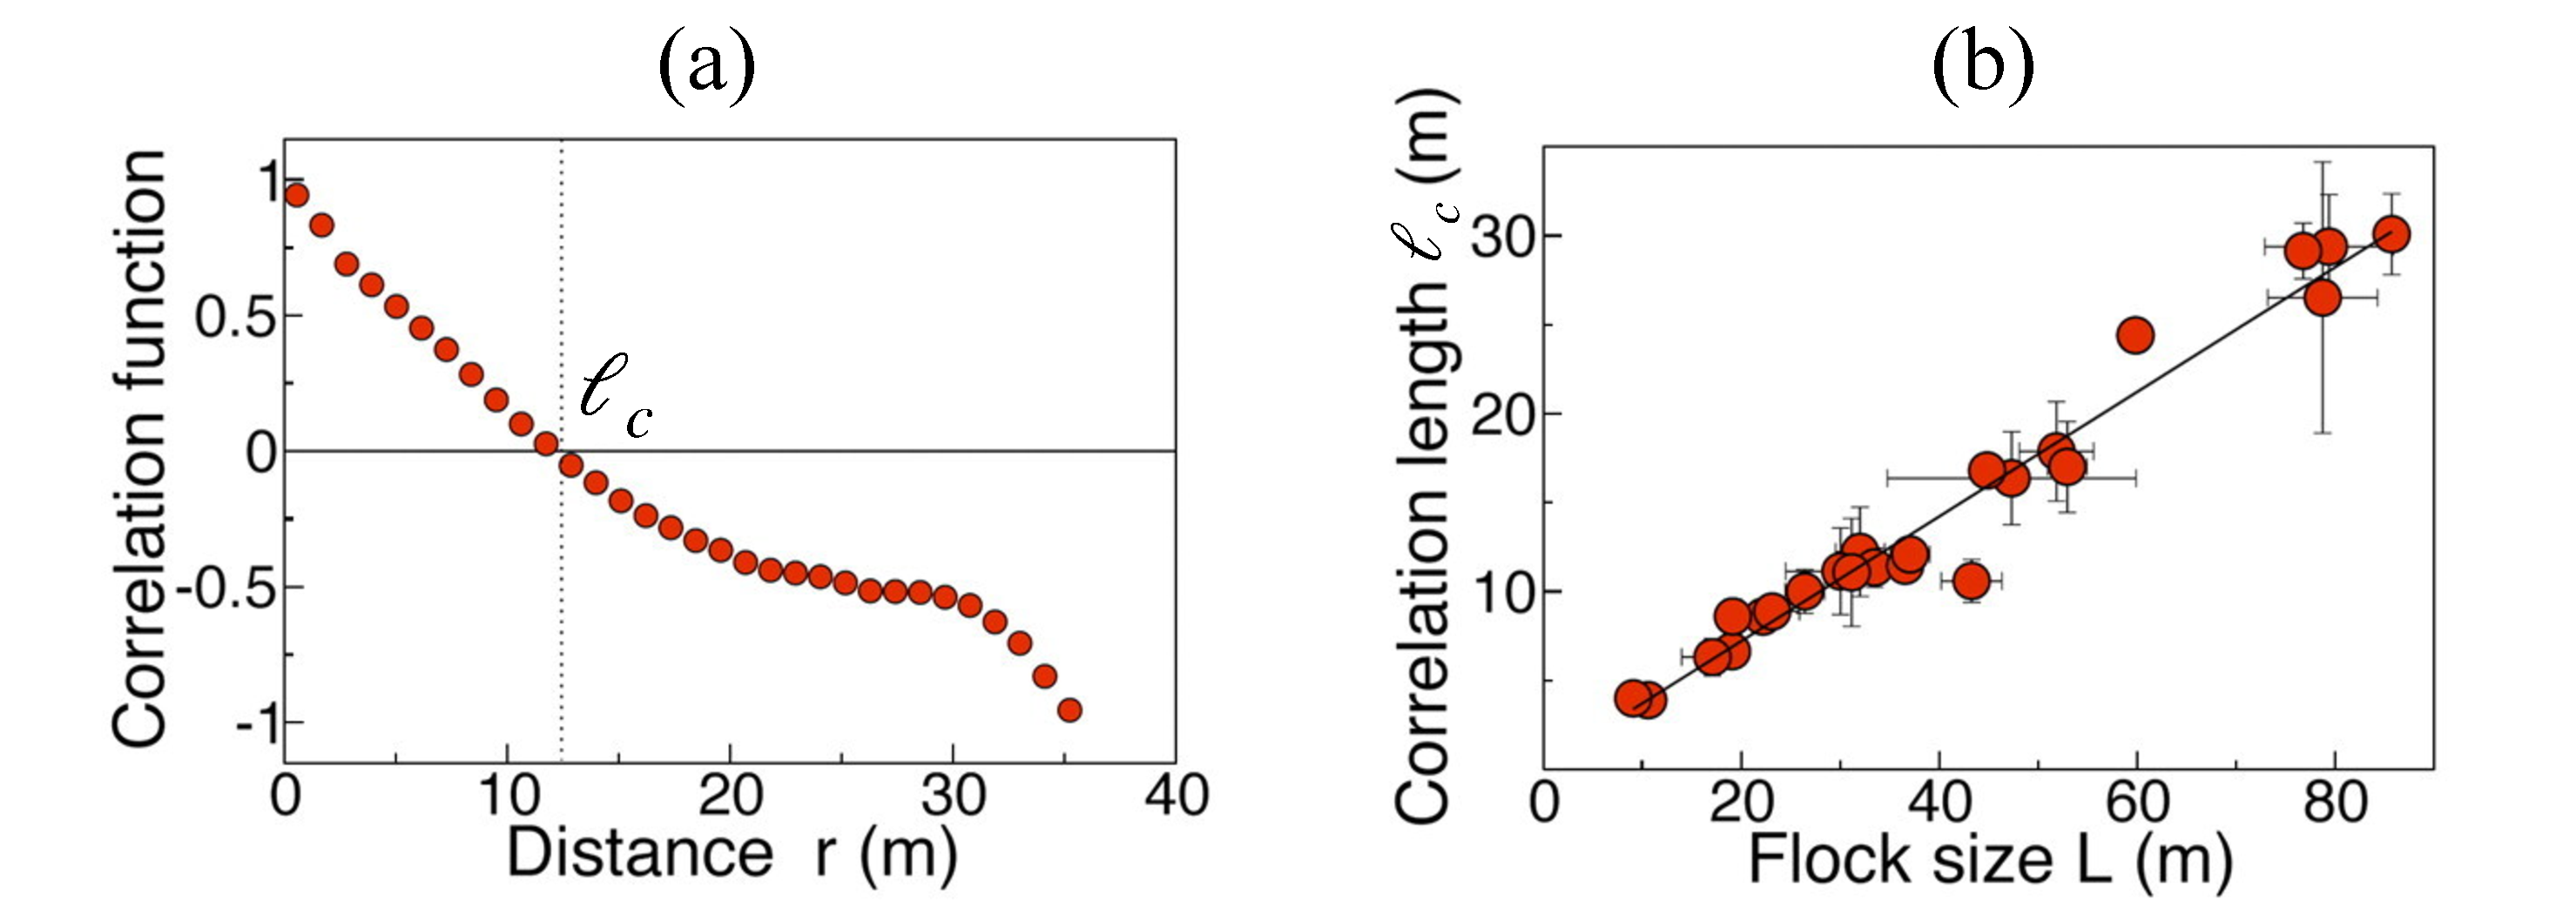
\includegraphics[width=.75\textwidth]{Figures/scalefree.pdf}
	\caption{(a) The correlation function $C(r)$ is the average inner product of the velocity fluctuations of pairs of birds at mutual distance $r$. This correlation function therefore measures to which extent the orientations of the velocity fluctuations are correlated. The function changes sign at $r=\ell_c$, which gives a good estimate of the average size of the correlated domains.(b) The orientation correlation length $\ell_c$ is plotted as a function of the linear size $L$ of the flock. Each point corresponds to a specific flocking event and it is an average over several instants of time in that event. The figure was reproduced from Ref.~\cite{cavagna2010scale}.
	}
	\label{scalefree}
	\end{center}
\end{figure}

Our purpose here will be to develop minimal models able to explain these features found not only in birds, but also in a variety of other systems.
Therefore, we will build our model from the example of birds for illustration purposes, but we won't consider the details of their ethology or morphology.
From far away, a flying bird is nothing but a polar object, meaning that is moves along a preferred direction set by its body axis.
Such feature is common in the systems we are interested in, so that in the following we will adopt an abstract representation
for which the bird is a simple arrow pointing along its direction of motion.

\paragraph*{Interactions with the environment}
Interactions between a biological systems and its environment are generally very complex and their quantitative description is here out of reach. 
Rather than solving the Navier-Stokes equations
to characterize the interaction of the bird with the surrounding air, 
we will here neglect inertia and the aerodynamics by assuming that the animal self-propels with a constant speed.
Such an approximation is arguably not so good for birds, but it turns out to be well verified for microscopic objects such as bacteria moving at low Reynolds numbers, or for any two dimensional active motion in the presence of a substrate.
Although setting the bird self propulsion speed to a constant leads to neglecting speed fluctuations, fluctuations in the direction of motion of the bird are generally still possible such that our model will retain orientational noise. 
 
 \paragraph*{Interactions with neighbors}
 Above, we have described the motion of a single bird, but below we will describe collective behaviors which implies to describe interactions between individuals.
 A prerequisite for flocking is that the birds seek to move together. 
 In the context of polar objects moving at constant speed, this effect is easily achieved via social rules leading to local alignment of velocities.
 Other types of interactions can of course be implemented. 
 For example, animals generally try to avoid colliding with each other, which can be described as a kind of short-ranged repulsion. Moreover, swarms or flocks usually show a certain degree of cohesion, which also suggests the presence of an effective attraction at long distances. 
 Another type of effective interactions may come from the medium our agents are moving into. An example of such interactions which we have studied in~\autoref{chap_phoretic} are phoretic interactions mediated by production/consumption and motility response to a chemical concentration. 
 Another prominent example are of course hydrodynamic interactions which play a central role in biological systems (cf~\autoref{chap_hydro}).
 Although these effects need to be considered when studying specific systems in details, they will enrich\footnote{Understand `complicate'.} the physics and may hide some of the universal features we are looking for. 
 In this lecture, we will thus restrict to the simplest setting where the agents of the model only interact via pairwise velocity alignment.


\section{The Vicsek model}

\subsection{Definition of the Vicsek class}

We now have all the necessary ingredients for a minimal model of collective motion.
The most famous one is arguably the Vicsek model~\cite{chate2020dry}, as it was first formulated by T. Vicsek and collaborators.
In the Vicsek setting, point-like particles move in two dimensions with constant speed $v_0$ and align their velocities with their neighbors in the presence of noise.
These rules mathematically translate in two dimensions into the following discrete time dynamics for the $i^{\rm th}$ particle's position $\bm r_i$ and velocity orientation $\theta_i$
\begin{subequations}
\label{eq_VM}
\begin{align}
\label{eq_VM_r}
\bm r_i^{t + \Delta t} & = \bm r_i^{t} + v_0 \Delta t \hat{\bm e}(\theta_i^{t + \Delta t}) \, , \\
\label{eq_VM_theta}
\theta_i^{t + \Delta t} & = {\rm Arg}\left[ \langle \hat{\bm e}(\theta_j^{t}) \rangle_{j \in \Omega_i} \right] + \eta \xi_i^t , 
\end{align}
\end{subequations} 
where $\hat{\bm e}(\theta) = (\cos(\theta),\sin(\theta))$ is the unit vector with orientation $\theta$, 
the average $\langle\cdot\rangle_{j \in \Omega_i}$ is done over the disk of radius $r_0$ centered in $i$: $\Omega_i \equiv \{ j ; \|\bm r_i  - \bm r_j\| \le r_0 \}$ 
(it therefore includes $i$ itself), and ${\rm Arg}[\bm v]$ returns the orientation of the vector $\bm v$.
The second term in the rhs of Eq.\eqref{eq_VM_theta} accounts for the angular fluctuations experienced by the particles, 
whose strength are set by the parameter $\eta$. 
$\xi_i^t$ is therefore a white noise with zero mean and unit variance:
$\langle \xi_i^t \xi_j^{t'} \rangle = \delta_{ij} \delta_{t t'}$ --hereafter angular brackets without indices are meant as averages over the noise.
In numerical simulations, the distribution of $\xi$ is usually taken uniform in $(-\pi;\pi]$ for simplicity, 
but other choices are possible (for instance Gaussian) and they do not qualitatively modify the dynamics 
so long as clockwise and counter-clockwise fluctuations remain equiprobable.
Similarly, different implementations of the Vicsek model have been proposed (e.g.\ considering continuous time dynamics, or with different forms of the noise etc...),
but those lead to large-scale collective features qualitatively similar to those of Eqs.~\eqref{eq_VM}.
For more details on the different numerical implementations of the Vicsek dynamics, see Ref.\cite{chate2020dry} and references therein.
Here, for practical purposes we'll consider the case where Eqs.~\eqref{eq_VM} are simulated in a square domain of linear size $L$ with periodic boundary conditions on all sides.

As for the Ising or $XY$ models for ferromagnets, the importance of the role of the Vicsek model in active matter studies stems from its simplicity and genericity.
Indeed, numerical and theoretical studies of the model allowed to uncover general physical principles which can be applied to a broad range of active matter systems.
In this context, Eqs.~\eqref{eq_VM} thus define a {\it Vicsek class} (or polar class), whose members all satisfy the following requirements:
\begin{itemize}
\item The alignment interactions between the particles are {\it local} and {\it polar}. 
Particles moreover do not point towards a preferred direction so that the dynamics is {\it isotropic}.  
\item {\it The particles are advected by their polarities.} 
While the polarity and velocity of Vicsek particles are identical, this constraint can be relaxed to some extent if the two remain coupled.
\item As a consequence of the previous point, the Vicsek class is inherently out of equilibrium. 
In particular, the dynamics does not conserve momemtum, so that it is not invariant by change of inertial frame and {\it Galilean symmetry is broken}.
\item The dynamics~\eqref{eq_VM} nevertheless {\it conserves the total particle number $N$} (there are no particle creation or annihilation).
\end{itemize}

\subsection{The phase diagram}

\label{sec_pd}

Rescaling space and time, we set $\Delta t$ and $r_0$ to unity. 
Therefore, the Vicsek model has three control parameters: $v_0$, $\eta$, and the mean particle density $\bar{\rho} \equiv N / L^2$.
Considering $v_0$ in a `reasonable' range --meaning not too small so that activity appears on scales accessible via simulations, 
or not too large so that the neighborhood of each particle is not completely randomized at each simulation step-- its specific value does not qualitatively affect the dynamics\footnote{Typically $v_0$ is taken between 0.1 and 1.}.
Hence, the dynamical behaviors of Vicsek particles can be explored tuning the remaining two parameters: the average particle density $\bar{\rho}$ and the strength of the noise $\eta$.

The phase diagram of the Vicsek model in the ($\bar{\rho}$,$\eta$) plane is shown in Fig.~\ref{figVM}(a). It includes three phases:
\begin{itemize}
\item At low particle densities and high noises, fluctuations dominate over alignment interactions and the system is thus globally disordered. 
Namely, the polarity and density correlations are exponential with a finite associated correlation length $\ell_c$. 
The system can thus be split into uncorrelated domains of linear size $> \ell_c$ so that from the law of large numbers the global polar order vanishes over large scales as
\begin{equation}
\Pi \equiv \langle \|\langle \hat{\bm e}(\theta_i^{t}) \rangle_{i=1\ldots N}\|\rangle_t \underset{L \gg \ell_c}{\sim} N^{-1/2} \sim L^{-1} .
\end{equation} 
\item At high densities and low noises, the mean number of neighbors of each particles is large enough so that the system forms 
a homogeneous ordered state in which particles move collectively along a randomly selected direction. 
This symmetry broken phase exhibits characteristic features such as scale free (power law) density and order correlations, 
as well as long-range orientational (polar) order.
Namely, as shown in Fig.~\ref{figVM}(c) the system's global polarization is found to decay with system size to a nonzero value $\Pi_\infty$, with power law finite-size corrections:
\begin{equation}
\label{eq_LRO}
\Pi \sim \Pi_{\infty} + A L^{-\omega} .
\end{equation} 
Here $\Pi_\infty$ and $A$ depend on the parameters $\bar{\rho}$ and $\eta$ and the details of the microscopic dynamics, 
while the exponent $\omega \simeq 2/3$~\cite{chate2020dry} is universal so that its value is the same throughout the homogeneous ordered phase and for all two dimensional systems in the Vicsek class (similarly to the critical exponents that we have used in~\autoref{chap_intro} to describe the transition to order in the Ising model).

Another peculiar feature of the ordered phase can be observed by measuring the statistics of the number of particle $n(t) \equiv \int_{\cal V}{\rm d}\bm r \, \sum_i \delta(\bm r - \bm r_i^t)$ into a sub-domain of volume $\cal V$.
Namely, measuring the mean and variance of $n$ in domains of increasing sizes one finds that
\begin{equation}
\langle \Delta n^2 \rangle \sim \langle n \rangle^\phi ,
\end{equation}
with $\phi \simeq 1.6$ (see Fig.~\ref{figVM}(c))~\cite{chate2020dry}. 
In a system with `normal' density fluctuations, the law of large number would impose that $\phi = 1$. 
Here, however, $\phi > 1$, i.e.\ the variance of $n$ grows faster than its mean, 
so that density fluctuations in the homogeneous ordered phase are deemed as `anomalous', or `giant'\footnote{Note that these giant density fluctuations are not related to any clustering phenomenon (e.g.\ like the motility induced phase separation discussed in~\autoref{chap_scalar}),
but instead due to the infinite correlation length of density fluctuations in an overall spatially homogeneous system.}.
\item Finally, contrary to magnetic systems at equilibrium (i.e.\ described by the Ising or $XY$ models) the transition to order in the Vicsek model does not occur via a second order transition but is best described as a phase separation scenario where elongated dense ordered liquid domains --which are usually referred to as \textit{bands}, see Fig.~\ref{figVM}(b)-- coexist with a dilute disordered gas.
Because of the coupling between density and order, these bands travel in the direction orthogonal to their axis.
They moreover have a well-defined width selected by the noise, so that their number grows with the mean particle density or system size,
and in large systems they arrange into a regular smectic configuration.
This {\it micro-phase separated} phase is thus distinct from the usual phase separation in which a single liquid domain occupies a macroscopic fraction of space and grows with density and system size.
\end{itemize}

%%%%%%%%%%%%%%%%%%%%%%%%%%%%
\begin{figure}[t!]
	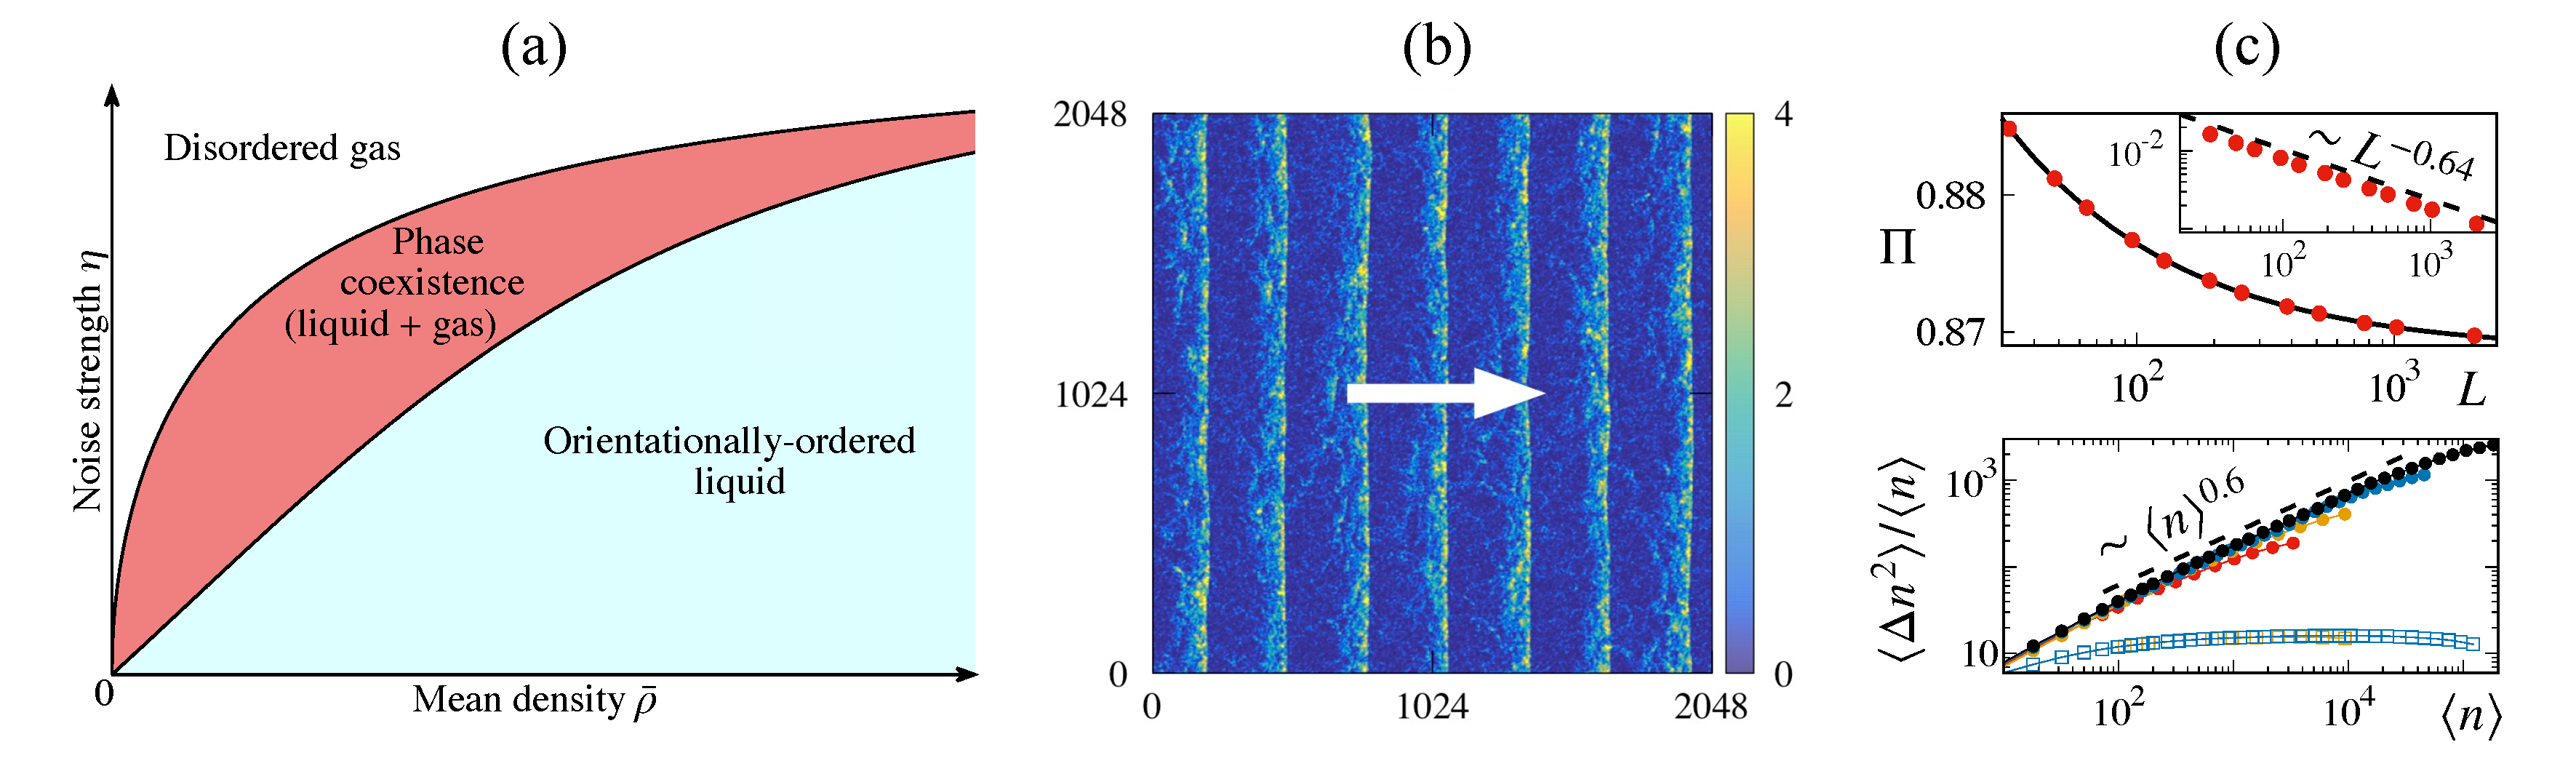
\includegraphics[width=\textwidth]{Figures/figVM.pdf}
	\caption{(a) The stylized phase diagram of the Vicsek model in the density-noise plane showing the three phases described in the text: disordered, homogeneously ordered, and the phase separated phase separating the two.
	(b) A snapshot of a regular smectic band configuration found in the phase-separated phase, the white arrow indicates the mean order direction and the color codes the local particle density. 
	Parameters are $\bar{\rho} = 1/2$, $\eta = 0.2$ and $v_0 = 0.5$.
	(c, top) Global polarization in the homogeneous ordered phase (in double-log representation) decreasing slower than a power law, the solid black line is a fit of the data by Eq.~\eqref{eq_LRO} giving $\Pi_\infty = 0.8685(2)$ and $\omega \simeq 0.64$. The inset shows the power law scaling of $\Pi - \Pi_\infty$ with system size.
	(c, bottom) $\langle \Delta n^2 \rangle/\langle n \rangle$ (see Sec.~\ref{sec_pd} for a definition) as a function of $\langle n \rangle$ showing anomalous density fluctuations in the ordered phase (filled circles) and normal fluctuations in the disordered phase (hollow squares). Different colors indicate different system sizes.
	Parameters for (c) are $\bar{\rho} = 2$, $v_0 = 0.5$, $\eta = 0.2$(ordered) and 0.6(disordered).
	All figures are reproduced from~\cite{DADAM_LesHouches}. 
	}
	\label{figVM}
\end{figure}
%%%%%%%%%%%%%%%%%%%%%%%%%%%%

\subsection{The hydrodynamic description of the Vicsek class}

It can be shown that a microscopic dynamics similar to that defined by Eqs.~\eqref{eq_VM} can be coarse-grained into hydrodynamic equations for the relevant physical fields which are the particle density $\rho$ and momentum $\bm w$ (or polarity):
\begin{align*}
\rho(\bm r,t) \equiv \left\langle \sum_i \delta(\bm r - \bm r_i^t) \right\rangle , \qquad 
\bm w(\bm r,t) = \rho(\bm r,t) \bm v(\bm r,t) \equiv \left\langle \sum_i \hat{\bm e}(\theta_i^t)\delta(\bm r - \bm r_i^t) \right\rangle .
\end{align*}
Using the Boltzmann-Ginzburg-Landau (BGL) approach detailed in Sec.~3 of Ref.~\cite{DADAM_LesHouches}, 
one can derive the set of partial differential equations governing the dynamics of $\rho$ and $\bm w$, known as the Toner Tu equations, which read
\begin{subequations}
\label{eq_TT}
\begin{align}
\label{eq_TT_rho}
& \partial_t \rho + \nabla \cdot \bm w = 0 , \\
\label{eq_TT_w}
& \partial_t \bm w + \lambda_1 (\bm w \cdot \nabla)\bm w + \lambda_2 (\nabla \cdot \bm w) \bm w + \lambda_3 \nabla |\bm w|^2 = 
-\frac{1}{2}\nabla \rho + \left( \mu(\rho) - \xi |\bm w|^2 \right) \bm w + \nu \Delta \bm w .
\end{align}
\end{subequations}
Thanks to the coarse-graining procedure, all coefficients of Eqs.~\eqref{eq_TT} can be expressed as functions of the microscopic dynamics parameters, i.e.\ density, noise and velocity.
This way it is possible to check from linear stability analysis and numerical simulations that Eqs.~\eqref{eq_TT} reproduce qualitatively the 
Vicsek model phase diagram of Fig.~\ref{figVM}(a) with the transition to collective motion occurring through a phase separated phase.
 
Although Eqs.~\eqref{eq_TT} were obtained starting from specific dynamical rules for the particles position and orientations, 
they contain almost all possible terms up to order 3 in fields and gradients that satisfy the constraints set by the Vicsek class,
so that their structure turns out to be quite generic and would not qualitatively change with the details of the dynamics.
In fact, Eqs.~\eqref{eq_TT} were first written by considering all relevant terms which satisfy the symmetries and conservation rules 
set by Eqs.~\eqref{eq_VM}:
\begin{itemize}
\item As a consequence of the particle number conservation, $\rho$ is a conserved field and Eq.~\eqref{eq_TT_rho} takes the form of a continuity equation with a mass flux $\bm w$, reflecting the fact that density is advected by order.
\item In Eq.~\eqref{eq_TT_w} the symmetry breaking associated with collective motion is accounted for by the Landau cubic term on the r.h.s. which, for $\mu(\bar{\rho}) > 0$, leads to the homogeneous ordered solution $\bm w = \sqrt{\mu(\bar{\rho}) / \xi} \hat{\bm e}_\|$ and $\hat{\bm e}_\|$ a unit vector pointing along an arbitrary direction.
\item The nonlinear terms on the l.h.s.\ of Eq.~\eqref{eq_TT_w} are moreover all allowed with arbitrary coefficients due to the absence 
of momentum conservation\footnote{In a compressible system, the advective term conserving momentum takes the form $\partial_t \bm w + \nabla \cdot (\bm w \bm w / \rho)$.}. 
Indeed, it is easy to check that they generally beak Galilean symmetry which would require the equations to be invariant under the transformation
\begin{equation*}
\bm w \to \bm w + \rho \bm u , \qquad \bm r \to \bm r - \bm u t ,
\end{equation*}
with $\bm u$ a constant velocity.
Moreover, because of these terms Eqs.~\eqref{eq_TT} generally cannot be written from minimizing of a free energy-type functional,
which highlights again the nonequilibrium nature of the underlying dynamics.
\end{itemize}
%Finally, we shall specify that the `simple' form of the pressure term ($\sim \nabla\rho$) in Eq.~\eqref{eq_TT_w} is a consequence of the point-wise nature of the particles, and considering short-range repulsion would lead to more a complicated expression. \\


In the remainder of these notes, we are going to focus on the derivation of large scale and long time universal properties of the fluctuating homogeneous ordered solution of Eqs.~\eqref{eq_TT}.
The approach presented below follows the seminal work by Toner and Tu~\cite{toner1995long,toner2012reanalysis}.
For readers interested in more details about the topic, we recommend the more recent treatment of Ref.~\cite{chate2024dynamic}.

\section{The transition to collective motion: linear stability analysis}

As Eqs.~\eqref{eq_TT} contain many terms which will not qualitatively affect the results derived below, 
for the sake of pedagogy we will study here simplified equations containing all relevant physical ingredients.
Namely, let us consider
\begin{subequations}
\label{eq_TT_new}
\begin{align}
\label{eq_TT_rho_new}
& \partial_t \rho + \nabla \cdot \bm w = 0 , \\
\label{eq_TT_w_new}
& \partial_t \bm w + \lambda (\bm w \cdot \nabla)\bm w = 
-\frac{1}{2}\nabla \rho + \left( \mu(\rho) - \xi |\bm w|^2 \right) \bm w + \nu \Delta \bm w ,
\end{align}
\end{subequations}
with now only one advection term in~\eqref{eq_TT_w_new}, but still with the coefficient $\lambda$ kept arbitrary.
Moreover, we will restrict most of the calculations to two dimensions.
For $\mu(\bar{\rho}) > 0$, the continuous theory admits the homogeneous ordered solution 
\begin{equation} \label{eq_hos}
\rho = \bar{\rho}, \qquad \bm w = \sqrt{\mu(\bar{\rho})/\xi} \hat{\bm e}_\| .
\end{equation}

In this section, we are interested in the stability of this solution.
We thus write the fields $\rho$ and $\bm w$ in terms of small perturbations around~\eqref{eq_hos}:
\begin{equation} 
\rho(\bm r,t) = \bar{\rho} + \delta\rho(\bm r,t), \qquad \bm w(\bm r,t) = \left( w_0 + \delta w_\|(\bm r,t) \right) \hat{\bm e}_\| + \delta w_\perp(\bm r,t) \hat{\bm e}_\perp ,
\end{equation}
with $w_0 \equiv \sqrt{\mu(\bar{\rho}) / \xi}$ and $\hat{\bm e}_\| \cdot \hat{\bm e}_\perp = 0$.
Keeping terms up to linear order, we obtain for the perturbations
\begin{subequations}
\label{eq_TT_lin}
\begin{align}
\label{eq_TT_lin_rho}
&\partial_t \delta \rho + \partial_\| \delta w_\| + \partial_\perp \delta w_\perp = 0, \\
\label{eq_TT_lin_para}
&\partial_t \delta w_\| + \lambda w_0  \partial_\| \delta w_\| = \left( \mu' w_0 - \frac{1}{2}\partial_\| \right)\delta \rho - 2\mu(\bar{\rho}) \delta w_\| + \nu \Delta \delta w_\| , \\
\label{eq_TT_lin_perp}
&\partial_t \delta w_\perp + \lambda w_0  \partial_\| \delta w_\perp =  - \frac{1}{2}\partial_\perp \delta \rho + \nu \Delta \delta w_\perp ,
\end{align}
\end{subequations}
where we have defined $\mu' \equiv {\rm d}\mu /{\rm d}\rho|_{\bar{\rho}}$ and $\partial_{\| , \perp} \equiv \hat{\bm e}_{\| , \perp} \cdot \nabla$.

Going into Fourier space, we recast Eqs.~\eqref{eq_TT_lin} into the linear system
\begin{equation*}
    \partial_t \begin{pmatrix}
        \delta\hat{\rho} \\
        \delta\hat{w}_\| \\
        \delta\hat{w}_\perp
    \end{pmatrix} = 
    \begin{pmatrix}
        0 & i q_\| & i q_\perp \\
        \mu'(\bar\rho)w_0 + \tfrac{1}{2}i q_\| & i\lambda w_0 q_\| - [2\mu(\bar\rho) + \nu q^2] & 0 \\
        \tfrac{1}{2}i q_\perp & 0 & i\lambda w_0 q_\| - \nu q^2
    \end{pmatrix}
    \begin{pmatrix}
        \delta\hat{\rho} \\
        \delta\hat{w}_\| \\
        \delta\hat{w}_\perp
    \end{pmatrix},
\end{equation*}
where $\delta\hat{\rho}(\bm q,t) = \int\dd\bm r \, \delta\rho(\bm r,t)\exp(i\bm q\cdot\bm r)$ and the other fields are defined in a similar way, while $\bm q = q_\|\hat{\bm e}_\| + q_\perp\hat{\bm e}_\perp$ with $q^2 = q_\|^2 + q_\perp^2$.
The stability of the homogeneous ordered solution is then set by the sign of the real part of the eigenvalue of the above matrix.

Given the configuration of the Vicsek bands (see~\autoref{figVM}), we moreover focus on perturbations in the direction longitudinal to the order here by setting $q_\perp = 0$.
This way, we directly obtain the eigenvalue associated to $\delta\hat{w}_\perp$: ${\cal Y}_\perp = -\nu q_\|^2 + i \lambda w_0 q_\|$,
whose real part is always negative.
The other two eigenvalues solve the second order polynomial equation
\begin{equation}\label{eq_poly_Y}
    {\cal Y}({\cal Y} + 2\mu(\bar\rho) + \nu q_\|^2 - i \lambda w_0 q_\|) - i q_\|\left(\mu'(\bar\rho) w_0 + \tfrac{1}{2}i q_\|\right) = 0.
\end{equation}
For $q_\| = 0$, it is straightforward to show that the solutions of this equation are ${\cal Y}_+ = 0$ and ${\cal Y}_- = -2\mu(\bar\rho)$.
As we are interested in long-wavelength instabilities, we focus here on ${\cal Y}_+$ and make use of the ansatz
\begin{equation*}
    {\rm Re}({\cal Y}) \underset{q_\| \to 0}{\simeq} q_\|^2, \qquad
    {\rm Im}({\cal Y}) \underset{q_\| \to 0}{\simeq} q_\|.
\end{equation*}
Replacing this ansatz in Eq.~\eqref{eq_poly_Y} we obtain at order $q_\|^2$
\begin{equation*}
    2 \mu(\bar\rho){\rm Re}({\cal Y}) - {\rm Im}^2({\cal Y}) + \lambda w_0 q_\| {\rm Im}({\cal Y}) + \tfrac{1}{2}q_\|^2 + i\left[ 2\mu(\bar\rho) {\rm Im}({\cal Y}) - q_\| \mu'(\bar\rho) w_0 \right] = 0,
\end{equation*}
from which we deduce
\begin{equation}
    {\rm Im}({\cal Y}) = \frac{\mu'(\bar\rho)w_0}{2\mu(\bar\rho)}q_\|, \qquad
    {\rm Re}({\cal Y}) = \frac{q_\|^2}{4\mu(\bar\rho)}\left[ \frac{(\mu'(\bar\rho))^2}{2 \mu(\bar\rho)\xi} - \frac{\lambda\mu'(\bar\rho)}{\xi} - 1 \right].
\end{equation}

\section{The Toner Tu theory: linearized hydrodynamics}

\subsection{Identification of the hydrodynamic modes}

Here, we consider a set of coefficients ($\lambda,\mu(\bar{\rho}),\xi,\nu$) so that we work deep enough in the ordered phase where~\eqref{eq_hos} is stable.
Comparing the r.h.s.\ of Eq.~\eqref{eq_TT_lin_para} with that of Eqs.~(\ref{eq_TT_lin_rho},\ref{eq_TT_lin_perp}), 
we find that $\delta w_\|$ is the only perturbation whose equation presents a damping term with coefficient $- 2\mu(\bar{\rho})$.
Consequently, longitudinal order perturbations typically relax on a finite timescale $\tau_\| \sim (2\mu(\bar{\rho}))^{-1}$,
while for density and transverse order perturbations are massless.
Therefore, $\delta w_\|$ can be considered as fast, 
while $\delta \rho$ and $\delta w_\perp$ are the hydrodynamic modes.

Using this separation of timescales between the fields, 
we neglect the time derivative in Eq.~\eqref{eq_TT_lin_para} and keep only the leading order terms in fields and gradients, which leads to
\begin{equation*}
\delta w_\| \simeq \frac{1}{2\mu(\bar{\rho})}\left( \mu' w_0 - \frac{1}{2}\partial_\| \right) \delta \rho .
\end{equation*}
Replacing this expression in Eq.~\eqref{eq_TT_lin_rho}, we finally get the closed set of equations
\begin{subequations}
\label{eq_TT_lin_closed}
\begin{align}
\label{eq_TT_lin_rho_closed}
&\partial_t \delta \rho + \tilde{v}_0\partial_\| \delta \rho + \partial_\perp \delta w_\perp = D_\rho \partial_\|^2 \delta\rho + \nabla \cdot \bm f_\rho, \\
\label{eq_TT_lin_perp_closed}
&\partial_t \delta w_\perp + \lambda w_0  \partial_\| \delta w_\perp =  - \frac{1}{2}\partial_\perp \delta \rho + \nu \Delta \delta w_\perp + f_\perp,
\end{align}
\end{subequations}
with $\tilde{v}_0 \equiv \mu' w_0 /  2\mu(\bar{\rho})$ and $D_\rho \equiv 1/4\mu(\bar{\rho})$.
As we are interested in calculating the response of the system to fluctuations, 
we have moreover included the noise terms $\bm f_\rho$ and $f_\perp$ in Eqs.~\eqref{eq_TT_lin_closed}.
We consider them as independent Gaussian white noises satisfying
\begin{equation} \label{eq_varf}
\langle f_{\rho,i}(\bm r,t)  f_{\rho,j}(\bm r',t') \rangle = \Delta_\rho \delta_{ij}\delta(\bm r - \bm r')\delta(t - t') , \qquad
\langle f_\perp(\bm r,t)f_\perp(\bm r',t') \rangle = \Delta_\perp \delta(\bm r - \bm r')\delta(t - t') .
\end{equation}
Note that the noise in Eq.~\eqref{eq_TT_lin_rho_closed} has to appear under a gradient term due to the particle number conservation constraint.

\subsection{Space-time correlations}

%\textcolor{blue}{I think that the FT has to be defined as $e^{-i(q \cdot r..)}$ to be consistent with the other formulas. I change it, in any case correct if it wrong. Also the term of the density noise misses an $i$.}

We now go to Fourier space:
\begin{equation*}
\delta \hat{\rho}(\bm q,\omega) = \int{\rm d}\bm r \int {\rm d}t \,  \delta\rho(\bm r,t)e^{i \bm q \cdot r - i \omega t} , \qquad
\delta \hat{w}_\perp(\bm q,\omega) = \int{\rm d}\bm r \int {\rm d}t \,  \delta w_\perp(\bm r,t)e^{i \bm q \cdot r - i \omega t},
\end{equation*}
where Eqs.~\eqref{eq_TT_lin_closed} are recast into the following linear system
\begin{equation}
\label{eq_TT_lin_fourier}
\begin{pmatrix}
\Gamma_\rho(\bm q,\omega) & -i q_\perp \\
-i\frac{q_\perp}{2} & \Gamma_\perp(\bm q,\omega) 
\end{pmatrix}
\begin{pmatrix}
\delta \hat{\rho}(\bm q,\omega) \\ \delta \hat{w}_\perp(\bm q,\omega)
\end{pmatrix}
=
\begin{pmatrix}
 -i\bm q \cdot \hat{ \bm f}_\rho(\bm q,\omega) \\ \hat{f}_\perp(\bm q,\omega)
\end{pmatrix} ,
\end{equation}
where $q_\|$ and $q_\perp$ are the wavenumbers associated respectively with the directions longitudinal and transverse to the global order, 
$\hat{ \bm f}_\rho$ and $\hat{f}_\perp$ are the Fourier transforms of the noises,
and we have defined 
\begin{equation*}
\Gamma_\rho(\bm q,\omega) \equiv i(\omega - \tilde{v}_0 q_\|) + D_\rho q_\|^2 , \qquad 
\Gamma_\perp(\bm q,\omega) \equiv i(\omega - \lambda w_0 q_\|) + \nu (q_\|^2 + q_\perp^2) .
\end{equation*}
In the following, we will focus on the scaling of the fields correlation functions in the large scale and long time limits, i.e.\ in the limits of vanishing $\omega$ and $q \equiv |\bm q|$.
In this regime the conserved noise term in Eq.~\eqref{eq_TT_lin_fourier} is subdominant w.r.t.\ $\hat{f}_\perp$, and we neglect it.
The system~\eqref{eq_TT_lin_fourier} is easily solved formally, and we find
\begin{equation}
\begin{pmatrix}
\delta \hat{\rho}(\bm q,\omega) \\ \delta \hat{w}_\perp(\bm q,\omega)
\end{pmatrix} = {\cal D}^{-1}(\bm q,\omega) 
\begin{pmatrix}
i q_\perp \\ \Gamma_\rho(\bm q,\omega)
\end{pmatrix} \hat{f}_\perp(\bm q,\omega) ,
\end{equation}
with ${\cal D}(\bm q,\omega) \equiv \Gamma_\rho(\bm q,\omega)\Gamma_\perp(\bm q,\omega) + q_\perp^2/2$.
In the limit where $\omega$ and $q$ go to zero, we simplify the expression of ${\cal D}(\bm q,\omega)$ by considering the following factorization
\begin{equation*}
{\cal D}(\bm q,\omega) \underset{\omega, q \to 0}{\simeq} -(\omega - \omega_+(\bm q))(\omega - \omega_-(\bm q)) ,
\end{equation*}
and where we assume that ${\rm Re}(\omega_\pm) \sim q$ and ${\rm Im}(\omega_\pm) \sim q^2$.
Replacing $w$ by $w_\pm(\bm q)$ in the expression of ${\cal D}(\bm q,\omega)$ and keeping terms up to order $q^2$ we end up with the dispersion relations 
$\omega_\pm(\bm q) = c_\pm(\theta_{\bm q}) q - i \varepsilon_\pm(\bm q)$, with
\begin{subequations}
\label{eq_speed_damp}
\begin{align}
\label{eq_speeds}
c_\pm(\theta_{\bm q}) &\equiv \frac{\lambda w_0 + \tilde{v}_0}{2}\cos(\theta_{\bm q}) \pm \sqrt{ \frac{(\lambda w_0 - \tilde{v}_0)^2}{4}\cos^2(\theta_{\bm q}) + \frac{\sin^2(\theta_{\bm q})}{2}} , \\
\label{eq_dampings}
\varepsilon_\pm(\bm q) &\equiv \frac{ [\tilde{v}_0\nu + D_\rho\lambda w_0\cos^2(\theta_{\bm q})  ]\cos(\theta_{\bm q}) - c_\pm(\theta_{\bm q})[\nu + D_\rho \cos(\theta_{\bm q}) ] }
{2 c_\pm(\theta_{\bm q}) + (\lambda w_0 + \tilde{v}_0)\cos(\theta_{\bm q}) } q^2 \sim q^2 ,
\end{align}
\end{subequations}
and where we have defined $\theta_{\bm q}$ as the angle between $\bm q$ and the global order ($q_\| = q\cos\theta_{\bm q}$ and $q_\perp = q\sin\theta_{\bm q}$). 
Using the expression of the noise variance in Fourier space $\langle \hat{f}_\perp(\bm q,\omega) \hat{f}_\perp(\bm q',\omega') \rangle = \Delta_\perp (2\pi)^3 \delta(\bm q + \bm q') \delta(\omega + \omega')$, we get the following expressions of the density and order correlation functions
\begin{subequations}
\label{eq_space_tim_cfs}
\begin{align}
\label{eq_space_tim_cfs_rho}
\left\langle \left|\delta \hat{\rho}(\bm q,\omega)\right|^2 \right\rangle &\underset{\omega, q \to 0}{\simeq} \frac{\Delta_\perp q_\perp^2}
{\left[ ( \omega - c_+(\theta_{\bm q}) q)^2  + \varepsilon^2_+(\bm q)   \right]\left[ ( \omega - c_-(\theta_{\bm q}) q)^2  + \varepsilon^2_-(\bm q)   \right]} , \\
\label{eq_space_tim_cfs_w}
\left\langle \left|\delta \hat{w}_\perp(\bm q,\omega)\right|^2 \right\rangle &\underset{\omega, q \to 0}{\simeq} \frac{\Delta_\perp (\omega - \tilde{v}_0 q_\|)^2}
{\left[ ( \omega - c_+(\theta_{\bm q}) q)^2  + \varepsilon^2_+(\bm q)   \right]\left[ ( \omega - c_-(\theta_{\bm q}) q)^2  + \varepsilon^2_-(\bm q)   \right]} .
\end{align}
\end{subequations}
As shown in Figs.~\ref{figmodes}(a,b), the density and order correlation functions plotted as function of $\omega$ at fixed $\bm q$ thus exhibit two peaks centred in $c_\pm(\theta_{\bm q})q$ and of widths $\varepsilon_\pm(\bm q)\sim q^2$.
Such structure reflects the presence of propagating density and order waves in the system with dispersion relations $\omega = \omega_\pm(\bm q)$.
Namely, these modes propagate with characteristic speeds $c_\pm(\theta_{\bm q})$ that depend on the orientation of $\bm q$ w.r.t.\ the mean order direction (see Fig.~\ref{figmodes}(c)). 
This is a direct consequence of fact that we are analyzing a symmetry broken phase.
Moreover, measuring the two different speeds of the modes in the direction longitudinal to order gives 
a direct indication of the absence of Galilean invariance in the system ($\tilde{v}_0 \ne \lambda w_0$).
The predicted life time of the modes takes a more conventional form set by $\varepsilon^{-1}_\pm(\bm q)\sim q^{-2} \sim \lambda^2$ with $\lambda$ the mode wavelength, which corresponds to the expected scaling for diffusive damping.

As we derived the structure of the propagating density and order modes from the generic hydrodynamic theory, 
we expect it to hold for a broad variety of systems.
Simulations of the Vicsek model~\eqref{eq_VM} indeed confirm the two-peaks structure predicted by Eqs.~\eqref{eq_space_tim_cfs}.
Measuring the peaks positions, one finds that they indeed scale linearly with $q$. 
The associated slope corresponds to the modes speeds which are found to vary with the orientation $\theta_{\bm q}$ 
in perfect agreement with Eq.~\eqref{eq_speeds} (as shown in Fig.~\ref{figmodes}(c)).
This phenomenology moreover holds beyond the Vicsek setting, as found in numerical simulations of a realistic model of self-propelled polar rods~\cite{Soni2020}
as well as in colloidal rollers experiments~\cite{geyer2018sounds}.

%%%%%%%%%%%%%%%%%%%%%%%%%%%%
\begin{figure}[t!]
	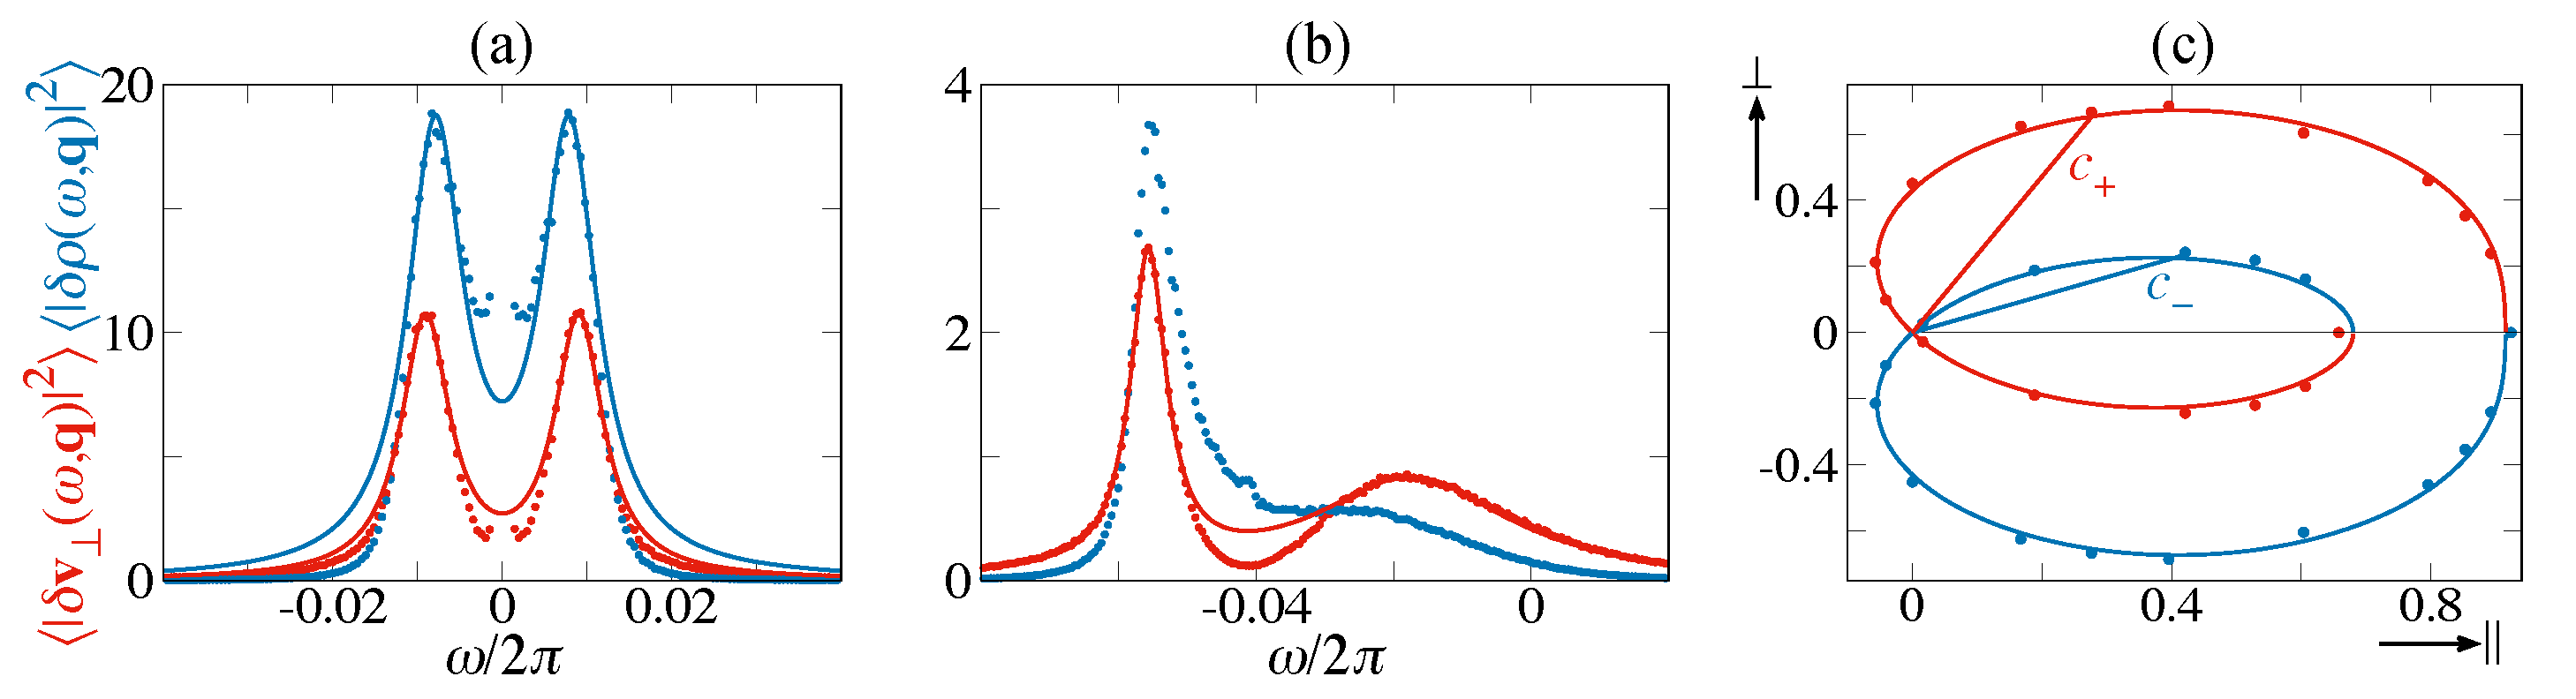
\includegraphics[width=\textwidth]{Figures/figmodes.pdf}
	\caption{(a,b) density(blue) and order(red) space time correlation functions as function of the frequency $\omega$ for $\theta_{\bm q} = \pi/2$(a) and $\pi/4$(b),
	respectively showing two symmetric and asymmetric peaks.
	When present, the continuous lines are fits of the numerical data (points) with Eqs.~\eqref{eq_space_tim_cfs}.
	(c) Polar representation of the mode speeds obtained from the scaling of the density and order correlation functions peaks position with $q$ at various values of $\theta_{\bm q}$. 
	The full line shows a fit of the data with Eq.~\eqref{eq_speeds}.}
	\label{figmodes}
\end{figure}
%%%%%%%%%%%%%%%%%%%%%%%%%%%%

\subsection{Equal-time correlation functions}

We now investigate on the nature of order as well as the presence of giant density fluctuations, which are both related to the equal-time correlation functions.
Equal-time density and order correlations are simply obtained by integrating Eqs.~\eqref{eq_space_tim_cfs} over the frequency $\omega$.
The full calculation can be carried out explicitly, but can be simplified considering the limit of small wavenumbers.
Indeed, although the two peaks in the space-time correlation functions are separated by $\sim q$, their respective widths $\sim q^2$ and their heights $\sim q^{-2}$.
Therefore, for $q \to 0$ the integral over $\omega$ of Eqs.~\eqref{eq_space_tim_cfs} will be dominated by the contributions from the individual peaks, 
which can be treated independently.
Using the relation $\int_{-\infty}^{+\infty} {\rm d}x \, [(x - x_0)^2 + \alpha^2]^{-1} = \pi/\alpha$, we thus get after little algebra
%\begin{subequations}
%\label{eq_eq_tim_cfs}
\begin{align*}
%\label{eq_eq_tim_cfs_rho}
\left\langle \left|\delta \hat{\rho}(\bm q)\right|^2 \right\rangle &\underset{q \to 0}{\simeq} \frac{\Delta_\perp \sin^2(\theta_{\bm q})}{ 2[c_+(\theta_{\bm q}) - c_-(\theta_{\bm q})]^2 }
\left( \frac{1}{\varepsilon_+(\bm q)} + \frac{1}{\varepsilon_-(\bm q)}  \right) , \\
%\label{eq_eq_tim_cfs_w}
\left\langle \left|\delta \hat{w}_\perp(\bm q)\right|^2 \right\rangle &\underset{q \to 0}{\simeq} \frac{\Delta_\perp}{ 2[c_+(\theta_{\bm q}) - c_-(\theta_{\bm q})]^2}
\left( \frac{ [ c_+(\theta_{\bm q}) - \tilde{v}_0\cos(\theta_{\bm q}) ]^2 }{\varepsilon_+(\bm q)} + \frac{[ c_-(\theta_{\bm q}) - \tilde{v}_0\cos(\theta_{\bm q}) ]^2}{\varepsilon_-(\bm q)}  \right) .
\end{align*}
%\end{subequations}
Using the expressions of the $c_\pm(\theta_{\bm q})$ and $\varepsilon_\pm(\bm q)$ given in Eq.~\eqref{eq_speed_damp} we finally rewrite these expressions into a more compact form:
\begin{equation}
\label{eq_eq_tim_cfs_simple}
\left\langle \left|\delta \hat{\rho}(\bm q)\right|^2 \right\rangle \underset{q \to 0}{\simeq} \frac{P_\rho(\theta_{\bm q})\sin^2(\theta_{\bm q})}{q^2} , \qquad
\left\langle \left|\delta \hat{w}_\perp(\bm q)\right|^2 \right\rangle \underset{q \to 0}{\simeq} \frac{P_\perp(\theta_{\bm q})}{q^2} ,
\end{equation}
with $P_\rho(\theta_{\bm q})$ and $P_\perp(\theta_{\bm q})$ two ${\cal O}(1)$ functions.
In agreement with numerical and experimental observations, density and order correlations are scale free (they scale like a power of $q$).
Moreover, although we derived Eqs.~\eqref{eq_eq_tim_cfs_simple} starting from a two dimensional theory, this result holds in arbitrary dimensions $d \ge 1$~\cite{toner2012reanalysis}.

\subsubsection{Giant density fluctuations}

The scaling of density fluctuations is obtained through the relation $\langle \Delta n^2 \rangle / \langle n \rangle \sim \lim_{q\to 0} \langle |\delta \hat{\rho}(\bm q)|^2 \rangle$.
Conventional density fluctuations are thus found when the Fourier space density correlation saturates to a constant value as $q \to 0$.
Here, on the contrary, $\langle |\delta \hat{\rho}(\bm q)|^2 \rangle$ diverges at vanishing wavenumbers like $q^{-2}$.
Using that $q \sim 1/L \sim 1/\langle n \rangle^{1/d}$, this implies
\begin{equation}
\langle \Delta n^2 \rangle \sim \langle n \rangle^\phi ,
\end{equation}
with $\phi = 1 + 2/d$.
Therefore, although our theory correctly predicts the existence of giant density fluctuations in all dimensions $d \ge 1$, 
the corresponding predicted exponent $\phi = 2$ for $d=2$ is larger than that measured in simulations or experiments (see e.g.\ Fig.~\ref{figVM}(c)).

\subsubsection{The nature of order}

For any dimension $d$, the typical strength of order fluctuations is set by 
\begin{equation}
\label{eq_order_flucts}
\left\langle \left|\delta {w}_\perp(\bm r)\right|^2 \right\rangle = \int \frac{{\rm d}\bm q}{(2\pi)^d} \left\langle \left|\delta \hat{w}_\perp(\bm q)\right|^2 \right\rangle 
\underset{q\to 0}{\sim} \int_{1/L}^{1/\Lambda} {\rm d}q \, q^{d-3} \underset{L\to +\infty}{\sim} 
\begin{cases}
L & (d=1) \\
\ln(L / \Lambda) & (d=2) \\
\Lambda^{2-d} & (d \ge 3)
\end{cases},
\end{equation}
with $\Lambda$ and ultra-violet cutoff length.
Eq.~\eqref{eq_order_flucts} predicts that the global polar order is destroyed by fluctuations in the limit of infinite system sizes for dimensions $d \le 2$.
More specifically, the logarithmic divergence predicted in $d=2$ is `slow enough' that, although the order vanishes asymptotically, the associated correlation length remains infinite.
Consequently, the global polarization decays with system size as $L^{-\kappa}$ with the exponent $0 < \kappa < 1$ usually nonuniversal.
This regime corresponds e.g.\ to that of the ordered phase of the two dimensional $XY$ model at equilibrium, and is named `quasi-long-range order'.
In $d \ge 3$, however, Eq.~\eqref{eq_order_flucts} predicts bounded polar order fluctuations so that order should remain long-ranged.\\
\\
In summary, we have derived the scaling of density and order correlation functions around the fluctuating homogeneous ordered solution of the Toner Tu equations~\eqref{eq_TT_new}.
The theory succeeds in predicting the presence of propagating density and order modes, giant density fluctuations, as well as the scale free correlations observed in numerical simulations and experiments.
However, some discrepancies persist: the exponent associated with giant density fluctuations is measured to be smaller than its predicted value, 
and most importantly the theory predicts a quasi-long-range order in two dimensions, 
at odds with observations of long-range orientational order~\eqref{eq_LRO} in numerical simulations of the two dimensional Vicsek model (see Fig.~\ref{figVM}(c)).
As we show below, these differences can be qualitatively explained by the fact that the effect of nonlinearities in the Toner Tu equations cannot be neglected in low dimensions, 
so that the linearized theory effectively breaks down.

\section{Some elements of the nonlinear Toner Tu theory}

To evaluate the importance of nonlinearities, we need to derive a nonlinear version of Eqs.~\eqref{eq_TT_lin_closed}.
Then, the question arises of which nonlinear terms should be kept and which should be discarded. The method to evaluate the relevance of these additional terms is called scaling analysis, or more formally the Renormalization Group (RG). 

The main idea behind this is the validity of the scaling hypothesis: when the system is largely correlated, i.e. $\ell_c \gg \Lambda$, the correlation length is the only relevant length scale of the dynamics, and it determines the macroscopic behavior through universal critical exponents. Indeed, all the microscopic details on scales smaller than $\ell_c$ do not really matter in a hydrodynamic description of the system. This is even more evident when $\ell_c \to \infty$, namely at the critical point of a phase transition or in the presence of spontaneous symmetry breaking with a Goldstone mode. In these cases, the system is scale invariant: the fluctuations extend on all the length scales (scale-free), and the physical properties are preserved when the observation scale is changed. To understand this, let's change the unit of space $r \to a r$, shrinking or dilating it with a scale factor $a$. We learned that when a system is scale-free, the correlation function of the order parameter decays with a power law $C(r) \sim r^{-\gamma}$. Performing the rescaling, we obtain
$$
C(ar) = \frac{1}{(ar)^{\gamma}} = a^{-\gamma} C(r) \ .
$$
The correlation function of the rescaled system is thus equal to the old correlation function multiplied by a constant factor: space rescaling does not change the physics when scale invariance is satisfied.  The RG is the set of transformations that allows to find the points of scale invariance (fixed points) of a specific field theory. It provides the information on how all the involved parameters have to change when space-time is rescaled, and the system is observed at larger and larger scales. 

We are now going to use RG arguments to understand which nonlinearities are relevant. For simplicity, we will consider here only the leading order nonlinearities, which are quadratic in the fields and linear in gradients. 
Carrying out the procedure detailed above, we find after enslaving the longitudinal order fluctuations\footnote{For the full derivation in the general case, see~\cite{toner2012reanalysis}.}
\begin{subequations}
\label{eq_TT_nlin_closed}
\begin{align}
\label{eq_TT_nlin_rho_closed}
&\partial_t \delta \rho + \tilde{v}_0\partial_\| \delta \rho + \partial_\perp \delta w_\perp + w_1 \partial_\perp( \delta \rho \delta w_\perp ) = 
D_\rho \partial_\|^2 \delta\rho + w_2\partial_\|  \delta \rho^2 + w_3 \partial_\|  \delta w_\perp^2 , \\
\label{eq_TT_nlin_perp_closed}
&\partial_t \delta w_\perp + \lambda w_0  \partial_\| \delta w_\perp + \lambda\delta w_\perp  \partial_\perp \delta w_\perp =  
- \frac{1}{2}\partial_\perp \delta \rho + \nu \Delta \delta w_\perp + g_1 \delta \rho \partial_\|  \delta w_\perp + g_2\delta w_\perp\partial_\|\delta \rho  + f_\perp,
\end{align}
\end{subequations}
and where, as previously, we have discarded the conserved noise term in Eq.~\eqref{eq_TT_nlin_rho_closed}.
Note, moreover, that all nonlinear terms in Eq.~\eqref{eq_TT_nlin_rho_closed} are total derivatives as a consequence of the particle number conservation.

We have shown from the linearized theory that the correlation functions of density and order in the ordered phase are scale free in $d\ge 2$,
therefore 
%from usual statistical mechanics arguments 
we assume the following scaling ansatz
\begin{equation} \label{eq_rescaling}
\bm r_\perp \to a \bm r_\perp , \quad r_\| \to a^\xi r_\| , \quad t \to a^z t , \quad \delta\rho \to a^{\chi_\rho}\delta\rho , \quad \delta w_\perp \to a^{\chi_\rho}\delta w_\perp ,
\end{equation}
with $a$ the given scaling factor.
The exponents $\xi$, $z$ $\chi_\rho$ and $\chi$ are {\it a priori} unknown, but as we will show below they can be fully determined for the linear theory.
$\xi$ measures the anisotropy of the scaling, while $\xi = 1$ corresponds to isotropy.
$z$ is called the dynamical exponent, and sets how the typical life time of perturbations scales with distances. 
$\chi_\rho$ and $\chi$ are the roughness exponents associated with density and order, respectively. 
They measure how the amplitude of fluctuations scales with distances. 

Applying the rescaling~\eqref{eq_rescaling} to Eqs.~\eqref{eq_TT_nlin_closed}, we get
\begin{subequations}
\label{eq_TT_rescalednonlin_closed}
\begin{align}
&\partial_t \delta \rho + \tilde{v}_0 a^{z-\xi} \partial_\| \delta \rho + a^{z + \chi - \chi_\rho -1} \partial_\perp \delta w_\perp + w_1 a^{z + \chi - 1} \partial_\perp( \delta \rho \delta w_\perp ) = \nonumber \\
& \qquad\qquad\qquad\qquad\qquad\qquad\qquad\qquad\qquad\qquad 
D_\rho a^{z-2\xi} \partial_\|^2 \delta\rho + w_2 a^{z + \chi_\rho - \xi}  \partial_\|  \delta \rho^2 + w_3 a^{z + 2\chi - \chi_\rho - \xi} \partial_\|  \delta w_\perp^2 , \\
&\partial_t \delta w_\perp + \lambda w_0 a^{z-\xi} \partial_\| \delta w_\perp + \lambda a^{z + \chi -1} \delta w_\perp  \partial_\perp \delta w_\perp  =  
- \frac{ a^{z + \chi_\rho - \chi - 1} }{2}\partial_\perp \delta \rho + \nu \left( a^{z-2\xi} \partial_\|^2 + a^{z-2} \partial_\perp^2 \right) \delta w_\perp \nonumber \\
& \qquad\qquad\qquad\qquad\qquad\qquad\qquad\qquad 
+ g_1 a^{z + \chi_\rho - \xi} \delta \rho \partial_\|  \delta w_\perp + g_2  a^{z + \chi_\rho - \xi} \delta w_\perp\partial_\|\delta \rho  + a^{\tfrac{z - 2\chi - (d-1) - \xi}{2}} f_\perp.
\end{align}
\end{subequations}
To calculate how the noise $f_\perp$ renormalizes upon the rescaling~\eqref{eq_rescaling}, we have used the relation~\eqref{eq_varf} 
as well as the fact that $\int {\rm d}\bm r' \, \delta(\bm r - \bm r') = 1$ and $ \int {\rm d}t' \, \delta(t - t') = 1$ must hold independently of $a$,
which implies $f_\perp^2 \to a ^{-(z + d-1 + \xi)} f_\perp^2$.
Each parameter of the theory could then be rescaled to preserve the same effective theory, for instance,
\begin{align*}
    D_\rho' &= D_\rho a^{z-2 \xi}, \\
    \nu' &= \nu a^{z-2}, \\
    \Delta_\perp' &= \Delta_\perp a^{(z-2\chi -(d-1)-\xi)/2}.
\end{align*}

To determine how the nonlinearities in Eqs.~\eqref{eq_TT_rescalednonlin_closed} renormalize upon the rescaling, 
we now evaluate the exponents in the linear theory. First, the continuity equation~\eqref{eq_TT_rho_new} combined with the dispersion relation $\omega \simeq c_\pm(\theta_{\bm q}) q$ implies that 
$c_\pm(\theta_{\bm q}) q \delta\hat{\rho} \sim q_\perp \delta \hat{w}_\perp$, which leads to $\chi_\rho = \chi$.
Secondly, the rescaling~\eqref{eq_rescaling} must leave the equal-time correlation functions~\eqref{eq_eq_tim_cfs_simple} invariant.
This can be achieved if the diffusion constants $\nu$ and $D_\rho$, as well as the noise $\Delta_\perp$, do not renormalize,
which from~\eqref{eq_TT_rescalednonlin_closed} implies the following hyperscaling relations
\begin{equation*}
z - 2 = 0, \qquad z - 2\xi = 0, \qquad z - 2\chi - (d-1) - \xi = 0 .
\end{equation*}
Solving for the three exponents, we then obtain their value given by the linear theory
\begin{equation}
z_{\rm lin} = 2, \qquad \xi_{\rm lin} = 1, \qquad \chi _{\rm lin} = 1 - \frac{d}{2} .
\end{equation}
In agreement with the results of the previous section, the linear theory thus predicts an isotropic scaling ($\xi = 1$), with diffusive damping of the modes ($z =2$)
and long-range order in $d \ge 3$ only ($\chi < 0$)\footnote{In two dimensions $\chi = 0$ but velocity correlations still diverge due to logarithmic corrections which cannot be captured by the scaling argument.}.

We now replace these values of the exponents in the nonlinear terms of  Eq.~\eqref{eq_TT_rescalednonlin_closed} to understand if the corresponding parameters grow or decrease upon rescaling. If they grow, the nonlinear terms are said to be {\it relevant} (positive scaling dimension), in the sense that they carry the system away from the linear fixed point. On the other hand, if they are irrelevant (negative scaling dimension) a small perturbation in their direction will be stable for the linear fixed point. We find that all nonlinearities renormalize as
\begin{equation}
\lambda; w_{1,2,3}; g_{1,2} \to a^{ \tfrac{4-d}{2} } \lambda; w_{1,2,3}; g_{1,2} .
\end{equation}
Therefore, for $d \ge 4$ all nonlinearities won't grow upon looking at the dynamics on larger scales. 
On the contrary, for $d < 4$ the strength of these nonlinearities grows as the theory is applied to larger scales and longer times, 
they are therefore relevant.
The upper critical dimension of the model, i.e.\ the dimension below which nonlinearities are important, is thus $d_c = 4$.

The the full nonlinear problem could be in principle addressed via renormalization group techniques, 
this is however a notoriously difficult task~\cite{toner2012reanalysis} which has not been performed so far.
Toner and Tu nevertheless managed to derive an expression for the scaling of the correlation functions using a matching procedure between the linear and nonlinear problems~\cite{toner1998flocks}.
They could show that the scaling of correlation functions could be obtained simply from their expressions~(\ref{eq_space_tim_cfs},\ref{eq_eq_tim_cfs_simple}) 
in the nonlinear theory with the renormalized noise variance and dampings
\begin{equation} \label{eq_renormalized_params}
\Delta_\perp(\bm q) = \Delta_\perp^0 q_\perp^{z - (d-1 + 2\chi + \xi)} {\cal F}_\Delta \left( \frac{q_\| }{q_\perp^\xi} \right) , \qquad
\varepsilon_\pm(\bm q) = \varepsilon_\pm^0 q_\perp^z {\cal F}_\pm \left( \frac{q_\| }{q_\perp^\xi} \right) ,
\end{equation}
while the modes speeds $c_\pm(\theta_{\bm q})$ remain those given by the linear theory, 
and where the functions ${\cal F}_\perp$ and ${\cal F}_\pm$ are unknown but universal and satisfy
\begin{equation*}
{\cal F}_\Delta(x) \underset{x \to 0}{\to} {\rm const} , \qquad {\cal F}_\Delta(x) \underset{x \to +\infty}{\to} x^{\tfrac{z - (d-1 + 2\chi + \xi)}{\xi}} ,\qquad
{\cal F}_\pm(x) \underset{x \to 0}{\to} {\rm const} , \qquad {\cal F}_\pm(x) \underset{x \to +\infty}{\to} x^{\tfrac{z}{\xi}} .
\end{equation*}
Replacing Eq.~\eqref{eq_renormalized_params} into Eq.~\eqref{eq_eq_tim_cfs_simple}, for instance, leads up to some ${\cal O}(1)$ factors
to the following expression of the equal-time correlation functions
\begin{equation} \label{eq_nl_scaling}
\left\langle \left|\delta \hat{\rho}(\bm q)\right|^2 \right\rangle \underset{q \to 0}{\simeq} \frac{q_\perp^{2 - (d-1 + 2\chi + \xi)}}{q^2}{\cal F}_\rho \left( \frac{q_\| }{q_\perp^\xi} \right)  , \qquad
\left\langle \left|\delta \hat{w}_\perp(\bm q)\right|^2 \right\rangle \underset{q \to 0}{\simeq} q_\perp^{- (d-1 + 2\chi + \xi)}{\cal F}_\perp \left( \frac{q_\| }{q_\perp^\xi} \right) ,
\end{equation}
with ${\cal F}_{\rho,\perp}(x) \underset{x \to 0}{\to} {\rm const}$ and  ${\cal F}_{\rho,\perp}(x) \underset{x \to 0}{\to} x^{\tfrac{- (d-1 + 2\chi + \xi)}{\xi}}$.
The scaling form~\eqref{eq_nl_scaling} was later confirmed by numerical simulations of the Vicsek model (for the full analysis, see~\cite{mahault2019TT}),
with the numerically determined exponents in two dimensions
\begin{equation} \label{eq_exps}
\chi = -0.31(2) , \qquad \xi = 0.95 (2) , \qquad  z = 1.33(2) .
\end{equation}
Therefore, it turns out that the scaling of correlation functions is nearly isotropic ($\xi \lesssim 1$), 
while the true long range order is confirmed ($\chi < 0$)\footnote{Actually, the exponent $\omega$ defined in Sec.~\ref{sec_pd} can be shown to be equal to $-2\chi$.}.
The fact that $z< 2$ moreover indicates that density and order fluctuations are damped 
on large scales more heavily than predicted by the linear theory (their life time scales as $\lambda^z$, with $\lambda$ their wavelength).
Going back to the giant density fluctuations, the exponents~\eqref{eq_exps} moreover imply that $\phi \simeq 1.67$, 
which is a value compatible with that usually directly measured from the scaling of $\langle \Delta n^2\rangle$ with $\langle n \rangle$ (see Fig.~\ref{figVM}(c)).

Although no proper RG treatment of Eqs.~\eqref{eq_TT_nlin_closed} has been carried out yet, recently alternative approaches based on scaling arguments have been proposed to predict the values of the exponents in dimension $d=2$.
Namely, the idea is first to note that for $\delta w_\perp$ to be a Goldstone mode, the deterministic part of its dynamics must be written as a total derivative (otherwise, the nonlinear terms that are not total derivatives effectively generate a mass), which implies in practice that $g_1 = g_2$.
As a consequence, the noise in Eq.~\eqref{eq_TT_nlin_perp_closed} cannot be renormalized by nonlinearities as the short scales of the theory are integrated out, since it is the only contribution on the r.h.s.\ that is not a total derivative. 
Hence, at the RG fixed point the hyperscaling relation
\begin{equation*}
    z = 1 + 2\chi + \xi,
\end{equation*}
must be satisfied.
Two other scaling relations can moreover be obtained by noting that Eqs.~\eqref{eq_TT_nlin_closed} remain invariant under a generalized Galilean transformation.
The details of this argument are quite subtle, so we refer to~\cite{chate2024dynamic} for details, but as a result the coefficients $w_{1,2,3},\lambda,g_1$ in front of the nonlinearities in Eqs.~\eqref{eq_TT_nlin_closed} are also not renormalized under RG transformation.
This implies two other scaling relations at the fixed point:
\begin{equation*}
    \chi + z - 1 = 0, \qquad
    \chi + z - \xi = 0.
\end{equation*}
Solving for $\chi$, $\xi$ and $z$, we then conclude that
\begin{equation}
    \chi = -\frac{1}{3}, \qquad
    \xi = 1, \qquad
    z = \frac{4}{3}.
\end{equation}
Note that these values are indeed very close to the ones obtained from numerical simulations (Eq.~\eqref{eq_exps}).

 % Appart from the giant density fluctuations, the scaling laws giving access to the values of the exponents $\chi$, $\xi$ and $z$ are difficult to measure
 % due to the strong finite size effects present in the Vicsek model. 
 % These effects are moreover amplified considering more realistic models with repulsion, or in experiments.
 % Therefore, for far there has not been any convincing experimental confirmation of the values of the exponents~\eqref{eq_exps}.


    \chapter{Nematic active matter  - Lectures 11\&12}
    \label{chap_nematic}
    %We will start with ``nematics'' before worrying about activity.
As discussed in \autoref{sec: momentum expansion} ``Nematics'' refere to systems with orientiational order but with no translational order.
urthere, there is no plarity.
This is illustrated in \autoref{fig: polar and nematic}.

Examples of Nematics are LCD screens.
Nematics are made of ``Rod-like objects'', like molecules that have a do-like shape a tthe smallest scale, like E-coli or bcillus subtillus.
One example is p-axoxynisole, illustrated in \autoref{fig: molecule}. \todo[noinline]{is this right}
Among al of these objects, the most common ``active nematic'' is Microtubule-kinesin system.
This system is active due to the walking of the  Kinesin motors.
The microtubules play the roles of rods, and their interactions create alignment.
The system is illustrated in \autoref{fig: micro-tubul}.

\begin{figure}[!htb]
    \centering
    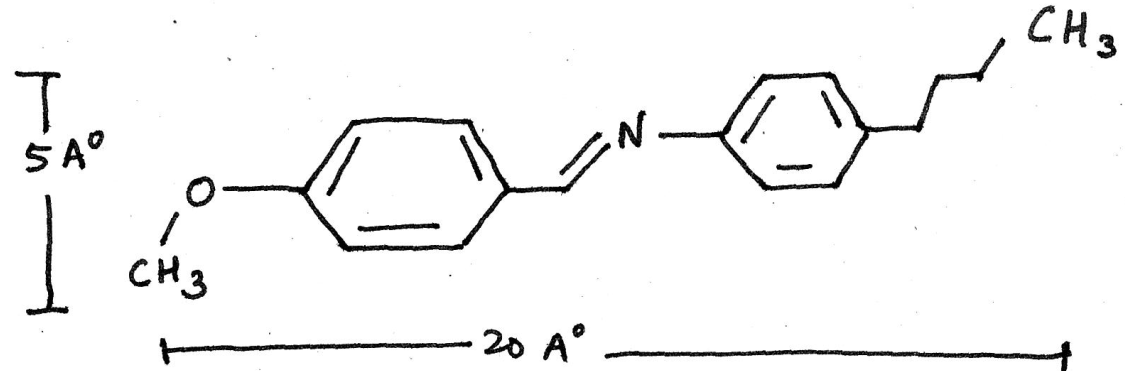
\includegraphics[width=.6\textwidth]{chapters/Figures/nematics/molecule.png}
    \caption{A rod-like molecule}
    \label{fig: molecule}
\end{figure}

\begin{figure}[!htb]
    \centering
    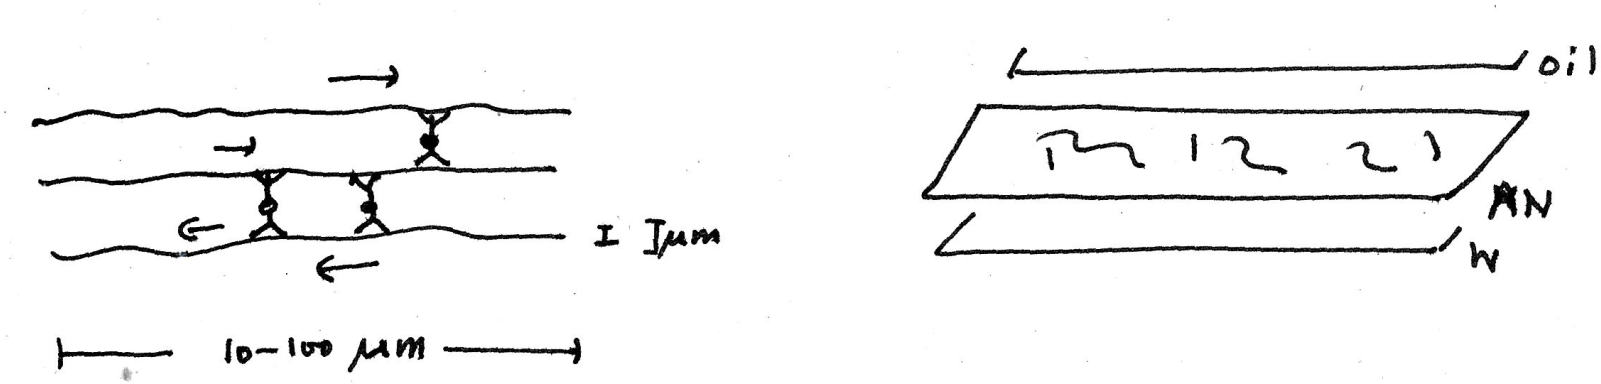
\includegraphics[width=.6\textwidth]{chapters/Figures/nematics/microtubules.png}
    \caption{A rod-like molecule}
    \label{fig: micro-tubul}
\end{figure}

What do you obtain from these experiments?
A continous churning of microtubules as long as you have ATP in the system.

Polar vs aplolar alignment can be ticky.It depends on some factors that have to be considered
For example, kinesin density, microtublue density, geometry of the boxe that confines the system.
In planar confinment, with a rectangular box, one achives nematic alignment, while a circular box give rise to polar order.
So the geometry and size matters.
Which brings us to the point that a system can be polar at small length/time-scales,, but at the level of hydrodynamic description, polarity might not survive.
It ``can vansih bacause of spatial averaging or time averaging''. (CITE COPENHAGEN 2021)

One may also consider a system of dry active nematics.
A experinatal setup is pointy rods, which are confined to a plane, and put on a shaker, as illustrated in \autoref{fig: shaker}.

\begin{figure}[!htb]
    \centering
    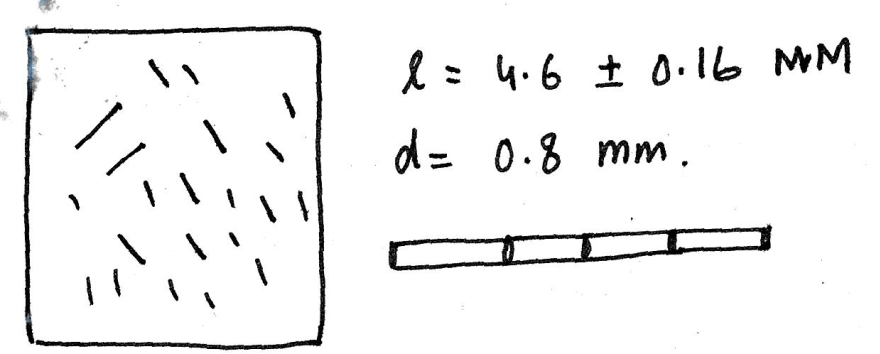
\includegraphics[width=.4\textwidth]{chapters/Figures/nematics/plate.png}
    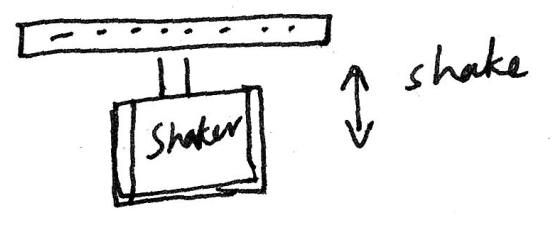
\includegraphics[width=.4\textwidth]{chapters/Figures/nematics/shaker.png}
    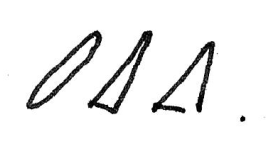
\includegraphics[width=.1\textwidth]{chapters/Figures/nematics/rods.png}
    \caption{The confined rods and shaker}
    \label{fig: shaker}
\end{figure}

In this lecture, we will ask the following questions:
Can active nematics have orientational order? 
What are the instabilities of such a system?
What roele does activity play?
In the first lecture, we will answer with a ery pictorial/qualitative resoning.
This is probably not very correct.
We then take a more systematic approach, to see what part of the qualitative approach survive.

\subsection*{Active nematic/polar activ swimmers in a fluid}

We begin by considering what happens to nematics when they act in a fluid.
As discussed in \autoref{sec: hydrodynamics of microswimmers} and in more details in \autoref{chap_hydro}, there are two types of swimmers, pushers and puelrs.
These creates different types of flow-fields, as illustrated in \autoref{fig: swimmers nematic}.
Which type of swimmer we are dealing with determine the sign of th active stress, and can have profound consequences in certain cases.

\begin{figure}[!htb]
    \centering
    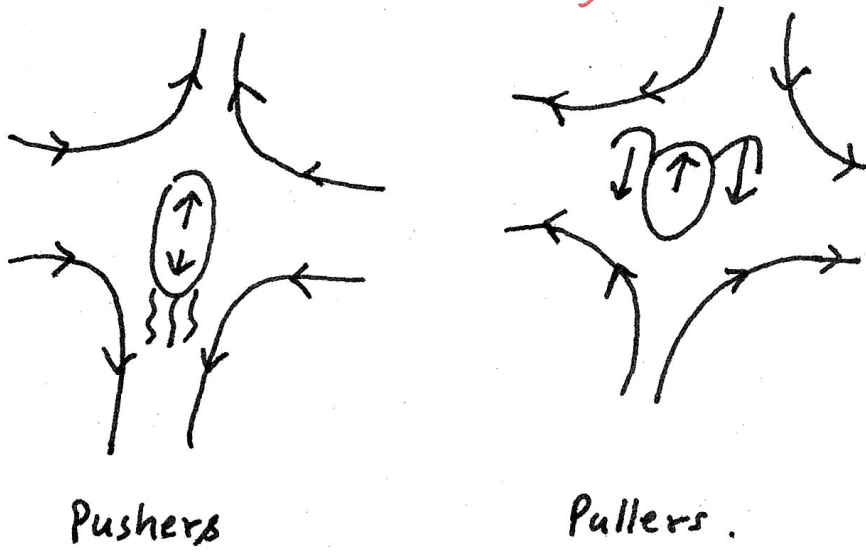
\includegraphics[width=.25\textwidth]{chapters/Figures/nematics/swimmers.png}
    \caption{Pushers and pullers create different flowfields}
    \label{fig: swimmers nematic}
\end{figure}

The microscopic models we sould have in mind are illustrated in \autoref{fig: kinesin}.

\begin{figure}[!htb]
    \centering
    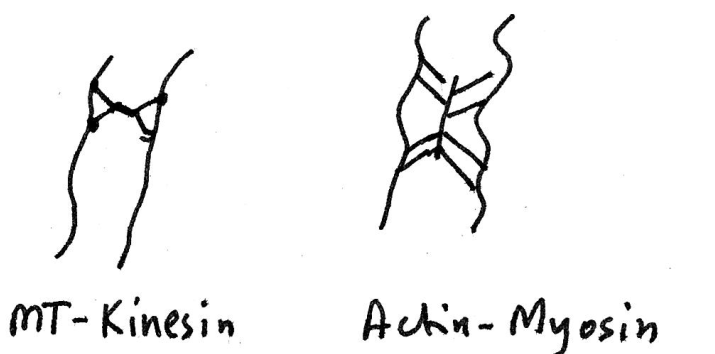
\includegraphics[width=.25\textwidth]{chapters/Figures/nematics/kinesin.png}
    \caption{Caption}
    \label{fig: kinesin}
\end{figure}

\section{Simha-Ramaswamy instability}

For a ordered state of swimmers/force dipoles, the total force will vanish, as illustrated in \autoref{fig: ordered dipoles}.
What happens when you add a bend/splay pertubation?
This velocity will try to reorient the dipoles, away from the inital state.
We see the two cases to in the middle and to the right in \autoref{fig: ordered dipoles}.
For the first case, the instability for the extensile force dipoles.
For the second case,
 contractile suspension hae a splay instability.
 What you get out of this is is simply ``active Turbulence''. 

\begin{figure}[!htb]
    \centering
    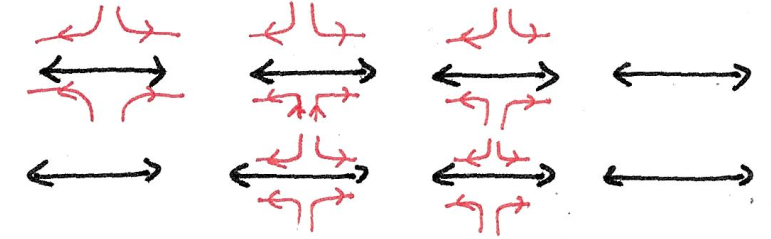
\includegraphics[width=.35\textwidth]{chapters/Figures/nematics/dipoles.png}
    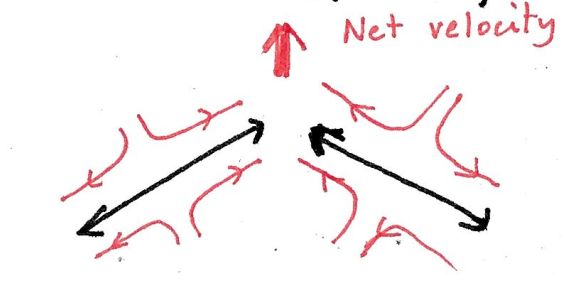
\includegraphics[width=.25\textwidth]{chapters/Figures/nematics/perturb1.png}
    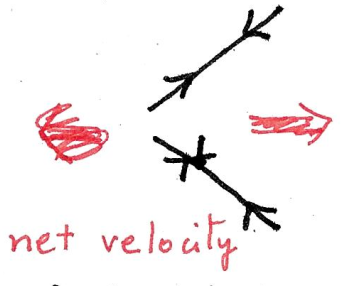
\includegraphics[width=.13\textwidth]{chapters/Figures/nematics/perturb2.png}
    \caption{The flow around ordered dipoles cancel out, leading to zero flow at large scales}
    \label{fig: ordered dipoles}
\end{figure}

\section{Finding the stresses on the fluid }

Recal the stokes equation,
%
\begin{align}
    0 &= \eta \nabla^2 \bm u - \bm \nabla P + \bm \nabla \cdot \Sigma, &
    \bm f = \bm \nabla \cdot \Sigma,
\end{align}
%
where $\Sigma$, the stress tensor, is a rank-2 tensor, and we have to find what it is.
If we consider force-dipoles with a forec $F$, the tensor should be proportional to $F$, the density of dipoles $c(\bm x, t)$, some length scale $\ell$ and something with ``OP''.\todo[noinline]{what?}

This, of course, only makes a scalar.
We have to also be able to create a rank-2 tensor.
IF we have polar order $\bm p$, we can make a tensor with $\bm p \otimes \bm p$, and the stress tensor becomes
%
\begin{align}
    \Sigma = A F \ell c(\bm x, t) \bm p(\bm x, t) \otimes \bm p (\bm x, t).
\end{align}
%
The sign of $A$ determins whether the force-dipole is extensile or contractile: $A<0$ means contractile, $A>0$ means extensile.
However, if there is no polar order, then this vanishes.
This brings us to ``nematics'' or the nemaic order parameter $Q$, as discuseed in \autoref{sec: momentum expansion}.
What does it need to respect?
The nematic symmetry.
Lets see how we can construct it.

\subsection*{The nematic order parameter}

Let $\bm \ell^\alpha$ be the unit vector for each particle, $\alpha \i \{1, \dots N\}$.
Then, 
%
\begin{align}
    \E{\bm \ell^\alpha}_\alpha = \frac{1}{N} \sum_{\alpha=1}^N \bm \ell^\alpha = 0.
\end{align}
%
Thus, $\E{\bm \ell}$ is no use to construct the nematic tensor.
We need to preserve the $\bm \ell^\alpha \leftrightarrow - \bm \ell^\alpha$ nematic symmetry.
The construction $\bm \ell^\alpha \cdot \bm \ell^\alpha$ is useless, since $\bm \ell^\alpha$ is defined as a unit vecotr.
Instead, we can define
%
\begin{align}
    Q_{ij}' = \E{(\bm \ell^\alpha \otimes \bm \ell^\alpha)_{ij}}_\alpha = \E{\ell^\alpha_i \ell^\alpha_j}_\alpha.
\end{align}
%
This is good, however
%
\begin{align}
    \mathrm{Tr} Q = 1,
\end{align}
%
always.
We want $Q$ to go to zero in the case where there is no alignment, so therefore we remove the trace,
%
\begin{align}
    Q_{ij} = \E{\ell^\alpha \cdot \ell^\alpha - \frac{1}{d}\one}.
\end{align}
%
 
Lets say there is perfect alignment along the $x$ axis, so $\ell^\alpha = (1, 0, 0)^T$.
Then, in three dimensions,
%
\begin{align}
    Q = 
    \begin{pmatrix}
        \frac{2}{3} & 0 & 0 \\
        0 & -\frac{1}{3} & 0 \\
        0 &0 & -\frac{1}{3}
    \end{pmatrix}.
\end{align}
%
In the isotropic phase, $Q = \frac{1}{d}\delta_{ij}$.
We see that $Q$ is a traceless, symmetric rank to tensor.
In two and three dimensions, these have the form
%
\begin{align}
    Q_{2\mathrm{D}} &= 
    \begin{pmatrix}
        a & b \\ b & -a
    \end{pmatrix}, &
    Q_{3\mathrm{D}} &= 
    \begin{pmatrix}
        a & c & d \\ c & b & e \\ d & e & - (a + b)
    \end{pmatrix}.
\end{align}
%


\subsection*{The scalar order parameter(???)}

\todo[inline]{there is a lot back and forth between dimensions, maybe do them one by one?}

$Q$ in 3 dimensions has 5 independent parameters.
Lets simplify our life a bit.
$Q$ is a symmetric traceless, so we can always diagonalize it, and the eigenvalues are real and the eigenvectors form an orthonormal basis.
We can write
%
\begin{align}
    \hat {\bm Q} = 
    \begin{pmatrix}
        \lambda_m & 0 & 0 \\ 0 & \lambda_s & 0 \\ 0 & 0 & - (\lambda_m + \lambda_s),
    \end{pmatrix}
\end{align}
%
where we assume that $\lambda_m$ is the larges eigenvalue. \todo[noinline]{Do we know they are positive?}

Let $\hat {\bm n}$ be an external reference vecotr, and $\theta^\alpha$ be the angle between $\bm \ell^\alpha$ and $\hat {\bm n}$.
Then, assuming uniaxial nematics, we can write
%
\begin{align}
    \hat Q_{xx} &= \E{\cos^2 \theta^\alpha - \frac{1}{3}}_\alpha&  \hat Q_{yy} & = \hat Q_{zz}.
\end{align}
%
THis means
%
\begin{align}
    \hat Q_{yy} =\hat Q_{zz} = - \frac{1}{2} \E{\cos^2\theta^\alpha - \frac{1}{3}}_\alpha.
\end{align}
%
We can thus write
%
\begin{align}
    Q &= 
    \begin{pmatrix}
        \frac{2}{3} & 0 & 0 \\
        0 & -\frac{1}{3} & 0 \\
        0 &0 & -\frac{1}{3}
    \end{pmatrix}S,&
    & S = \frac{1}{2} \E{3 \cos^2\theta^\alpha - \frac{1}{3}}_\alpha.
\end{align}
%
In two dimensions, we have
%
\begin{align}
    \hat Q = 
    \begin{pmatrix}
        \frac{1}{2} & 0 \\ 0 & - \frac{1}{2}
    \end{pmatrix}S, &&
    S = \E{\cos 2 \theta^\alpha}_\alpha.
\end{align}
%
 
In three dimensions, if $f(\theta, \phi)$ is the probability distribution of finding a single \emph{nematogen} at an orientation $(\theta, \phi)$, then
%
\begin{align}
    \E{\dots} = \int \dd \phi \int \dd \theta f(\theta, \phi) (\dots) \sin \theta  = 2 \pi \in \dd \theta f(\theta)(\dots) \sin \theta,
\end{align}
%
For perfect order,
%
\begin{align}
    f(\theta) = \frac{1}{2} [\delta(\theta) + \delta(\theta - \pi)] \implies S = 1,
\end{align}
%
while disorder means
%
\begin{align}
    f(\theta) = \const \implies \E{\cos^2\theta} = \frac{1}{3} \implies s = 0.
\end{align}
%
In general, we can write
%
\begin{align}
    Q = \frac{d}{d - 1}(\hat {\bm n} \otimes \hat {\bm n} - \frac{1}{d} \one).
\end{align}
%

In two dimensions, there is only one angle required to specify orientiation,
%
\begin{align}
    Q = s 
    \begin{pmatrix}
        \cos 2 \theta & \sin 2 \theta \\ \sin 2 \theta & - \cos 2 \theta
    \end{pmatrix}.
\end{align}
%

So, given $s(r)$ and $\hat {\bm n}(r)$, we can characterize the nematics.
$s(r)$ is the degree of alignment, while $\hat {\bm n}(r)$ is the direction in which this alignment is pointing.
If $\hat {\bm n}(r)$ is defined with respect to a rixed reference frame, then
\begin{align}
    Q = \frac{d}{d - 1}(\hat {\bm n} \otimes \hat {\bm n} - \frac{1}{d} \one).
\end{align}
%
\todo[inline]{I can't see what the difference to the earlier equation is supposed to be here\dots}

\section{Active Hydrodynamics}

Take the sotkes equation,
%
\begin{align}
    0 &= \eta \nabla^2 \bm u - \bm \nabla P + \bm \nabla \cdot \Sigma, &
    \partial_t \rho + \bm \nabla \cdot (\rho \bm u) &= 0.
\end{align}
%
We can split the stress tensor itno an active and a passive part,
%
\begin{align}
    \Sigma &= \Sigma^a + \Sigma^\gamma, &
    \Sigma^a = F \ell c(\bm x, t) Q(\bm x, t).
\end{align}
%
The passive part $\Sigma^\gamma$ comes from free energy arguments.
We will deal with it in some  time
the conentration equation is the conservation equation,
%
\begin{align}
    \partial_t c = \bm \nabla \cdot (c \bm u) = 0,
\end{align}
%
which for $c = \const$ give $\bm \nabla \cdot \bm u = 0$, which is incompressibility.
The equation for the nematic tensor is
%
\begin{align}
    \partial_t Q + \bm u  \cdot \bm \nabla Q = S - \Gamma M,
\end{align}
%
where $S$ are the flow couplings, and $M$ comes from free energy principles, which give rie to collective behavior and alignment.
To build a free eneryg, we consider that $F$ is a scalar.
We have to build it out of scalar invariants of the nemaitc tensor, the eigenvalues $\lambda_1$, $\lambda_2$ and $\lambda_3$
These follow
%
\begin{align}
    Q - \lambda_i \one = 0 \implies \lambda^3 - I \lambda^2 + I_2 \lambda - I_3 = 0.
\end{align}
%
In terms of trace and determinant of $Q$ these can be written
%
\begin{align}
    I_1 &= \mathrm{Tr}(Q) = \sum_i \lambda_i, \\
    I_2 & = \frac{1}{2} \left[\mathrm{Tr}(Q)^2 - \mathrm{Tr}(Q^2)\right]  = \lambda_1 \lambda_2 + \lambda_2 \lambda_3 + \lambda_3 \lambda_1, \\
    I_3 & = \mathrm{det}(Q) = \lambda_1 \lambda_2 \lambda_3.
\end{align}
%
With this, we get
%
\begin{align}
    F = \int \dd x \left[
        \frac{1}{2} a \mathrm{Tr}Q^2 - \frac{1}{3}b \mathrm{Tr}Q^3 + \frac{1}{4}c \left(\mathrm{Tr}Q^2\right)^2 + \frac{1}{2}K|\nabla Q|^2
    \right].
\end{align}
%

    \appendix

    \chapter{Some basics on equilibrium phase separation}
    \label{chapter: phase sep}

From now one and for simplicity, we will restrict the presentation to the case of a scalar mobility $M(\phi) > 0$.

\noindent {\it Spinodal decomposition} First, we can investigate the condition for a homogeneous configuration with $\phi = \bphi$ to be linearly stable.
Writing $\phi(\bm r,t) = \bphi + \delta \phi(\bm r,t)$, the perturbations $\delta \phi(\bm r,t)$ obey at linear order
\begin{equation} \label{eq_linear_phi}
\partial_t \delta \phi(\bm r,t) = \bar{M} \nabla^2 \left[ \left( \bar{f}'' - \bar{\kappa} \nabla^2\right)\delta \phi(\bm r,t)\right],
\end{equation}
where the bars stand for quantities evaluated at $\bphi$. 
Going into Fourier space, the growth rate associated to the mode with wavenumber $q$ is therefore $\lambda_q = -\bar{M} q^2(\bar{f}'' + \bar{\kappa} q^2)$.
As $\bar{M}$ and $\bar{\kappa}$ are both positive, the homogeneous configuration becomes unstable whenever $\bar{f}'' < 0$. 
This condition defines the so-called spinodals in the $(\bphi, k_B T$) phase diagram (Fig.~\ref{figeq}). 

%%%%%%%%%%%%%%%%%%%%%%%%%%%%
\begin{figure}[ht!]
	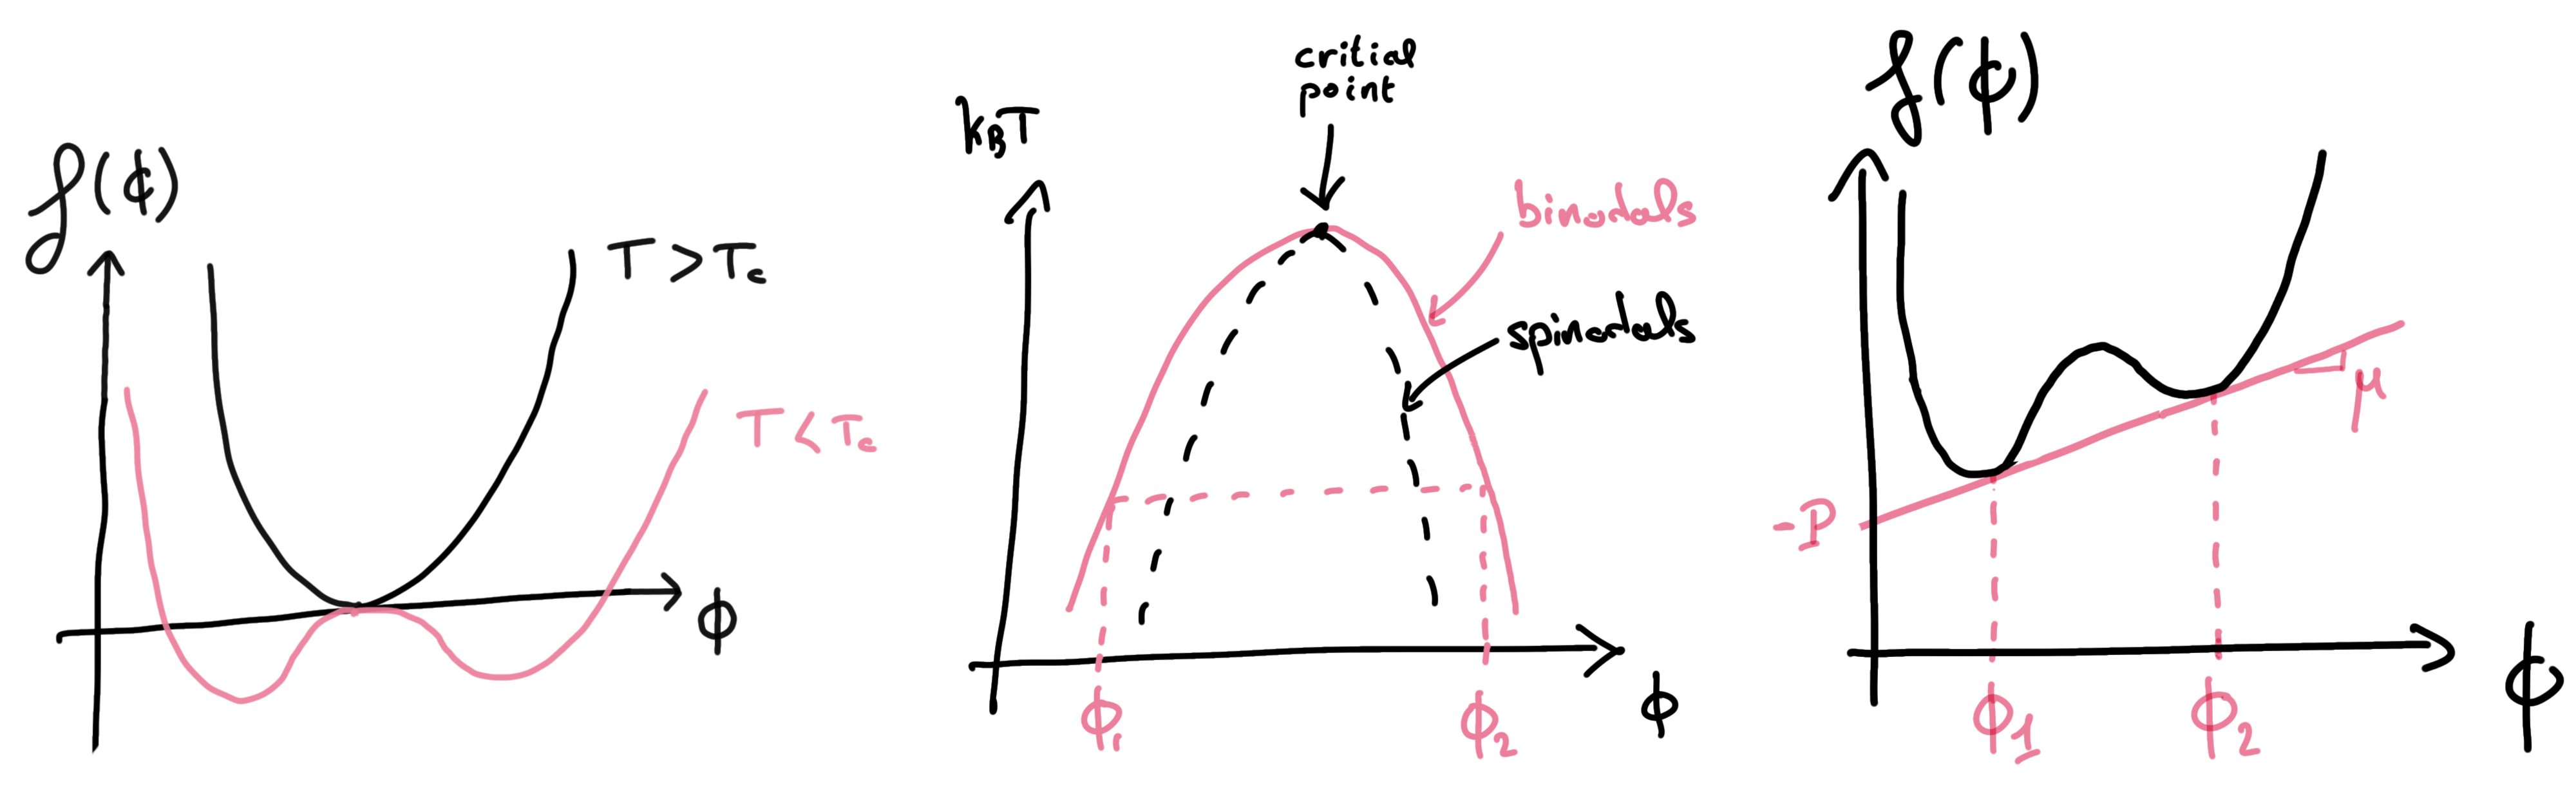
\includegraphics[width=\textwidth]{Figures/equilibrium_ps.pdf}
	\caption{Left: Typical Landau free energy landscapes above and below the critical point. 
	Center: phase diagram in the temperature $\phi$ plane showing the spinodals, binodals and critical point. 
	Right: Common tangent construction allowing to determine the coexistence densities in the phase separated regime.}
	\label{figeq}
\end{figure}
%%%%%%%%%%%%%%%%%%%%%%%%%%%%

\noindent {\it Binodals and the composition of phase separated configurations} 
The linear stability analysis and determination of the spinodals does not tell us anything about the asymptotic ($t \to \infty$) state of the system.
After the system undergoes spinodal decomposition, it goes through a coarsening regime until it phase separates into coexisting domains with different volumes and densities.
To determine the coexisting densities, we use the conservations of the total volume ${\cal V}$ and of the field $\phi$. 
We moreover work in the thermodynamic limit ${\cal V} \to \infty$ such that contributions from the interfaces can be safely neglected and we only consider the bulk contribution $f(\phi)$.
In a stationary phase separated regime where the system is partitioned into two domains with $\phi = \phi_{1,2}$ and of respective volumes ${\cal V}_{1,2}$, 
the free energy~\eqref{eq_F} thus takes the form
\begin{equation} \label{eq_F_ps}
{\cal F} = f(\phi_1) {\cal V}_1 + f(\phi_2) {\cal V}_2,
\end{equation} 
while denoting the mean value of $\phi$ as $\bphi$ the conservation constraints give
\begin{equation} \label{eq_constraints_binodals}
\phi_1 {\cal V}_1 + \phi_2 {\cal V}_2 = \bphi {\cal V}, \qquad  {\cal V}_1 + {\cal V}_2 = {\cal V} .
\end{equation} 
To determine the values $\phi_1$ and $\phi_2$, we can thus minimize the free energy~\eqref{eq_F_ps} imposing~\eqref{eq_constraints_binodals}.
This is done by adding the Lagrange multipliers ($\mu,P$) to ${\cal F}$, such that we define $\tilde{\cal F} = {\cal F} + P({\cal V}_1 + {\cal V}_2) - \mu(\phi_1 {\cal V}_1 + \phi_2 {\cal V}_2)$.
Minimizing $\tilde{\cal F}$ wrt the values of $\phi$ and volume for each of the two populations, we get
\begin{align} \label{eq_binodal_mu}
\frac{\partial \tilde{\cal F}}{\partial \phi_i}  & = {\cal V}_i (f'(\phi_i) - \mu) = 0 , \\
\label{eq_binodal_P}
\frac{\partial \tilde{\cal F}}{\partial {\cal V}_i}  & = f(\phi_i) - \mu \phi_i + P = 0 ,
\end{align}
with $i = 1,2$.
Eq.~\eqref{eq_binodal_mu} thus imposes that the chemical potential $\mu = f'(\phi_1) = f'(\phi_2)$ takes identical values in both phases (\emph{diffusive equilibrium}),
while Eq.~\eqref{eq_binodal_P} ensures the equality of pressures (\emph{mechanical equilibrium}).
Therefore, one can thus determine graphically the values of $\phi_1$ and $\phi_2$ from a common tangent construction 
on the free energy landscape. 
Indeed, the equality of chemical potentials imposes equal slopes of $f$ at $\phi_1$ and $\phi_2$, 
while equality of pressures imposes a common intercept on the vertical axis as shown in Fig.~\ref{figeq}

Varying e.g.\ the system temperatures, the coexistence values $\phi_{1,2}$ define the \emph{binodal curves},
and meet the spinodals we determined previously at the critical point. 
As shown in Fig.~\ref{figeq}, the spinodals and binodals generally do not coincide, such that there are regions of the phase diagram 
where phase separated configurations exist (and are stable) but the homogeneous state at $\phi = \bphi$ is also linearly stable.
In practice, if we now put back noise into the picture in these regions the homogeneous state will typically disappear 
not through the deterministic growth of an infinitesimal perturbation, 
but because of stochastic nucleation events which correspond to large perturbations and thus cannot be captured by linear stability analysis.
At fixed temperature below $T_c$ and for $\bphi$ lying in between the binodals, the system thus always phase separates over long times into two distinct domains 
where $\phi$ takes values $\phi_{1,2}$ and whose volumes linearly interpolate between 0 and ${\cal V}$ for $\bphi \in [\phi_1;\phi_2]$ due to the condition~\eqref{eq_constraints_binodals}, 
namely
\begin{equation}
{\cal V}_1 = \frac{\phi_2 - \bphi}{\phi_2 - \phi_1} {\cal V}, \qquad {\cal V}_2 = {\cal V} - {\cal V}_1 = \frac{\bphi - \phi_1}{\phi_2 - \phi_1} {\cal V},
\end{equation} 
which is known as the \emph{lever rule}.\\

\noindent {\it The coarsening dynamics} So far, we have discussed the linear instability of homogeneous solutions and the relative composition of phase separated phases.
Of course, another interesting aspect of phase separation concerns how one moves from one to the other. 
Without entering into details (for the interested reader see~\cite{Bray1994}), 
the coarsening process leading to phase separation can be understood by taking into account finite size effects, 
i.e.\ by considering the nonlocal contributions to the free energy which were neglected above.
Doing this, one finds that the pressure inside a spherical droplet increases with its interface curvature, 
leading to a diffusive flux from small to large droplets. 
Over long times, small droplets thus typically shrink at the expense of larger ones which is known as \emph{Ostwald ripening}.
One can moreover show that under this process the mean droplet radius universally grows as $\sim t^{1/3}$,
while the asymptotic ($t \to \infty$) state inevitably consists of two macroscopic phase separated domains. 














\section{Passive model B and Cahn-Hilliard dynamics}

\label{sec_PMB}

\subsection{The dynamical theory for conserved scalar order parameter} 

We learned from statistical mechanics that the large-scale dynamics of systems that microscopically obey detailed balance minimize a free energy.
Therefore, model B is generally written in terms of a functional ${\cal F}[\phi]$, whose expression can be generally\footnote{You can consider other terms up to order $|\nabla \phi|^2$, 
and then think of why they cannot be allowed in the expression of ${\cal F}$.} expressed as
%
\begin{equation} \label{eq_F}
{\cal F}[\phi] = \intd{r} \left[ f(\phi) + \frac{\kappa(\phi)}{2}|\nabla\phi|^2\right],
\end{equation} 
%
where we have kept terms up to order $|\nabla \phi|^2$.
In Eq.~\eqref{eq_F} $f$ denotes the `bulk' free energy density and $\kappa(\phi) > 0$ a generic constant.
The bulk contribution consists of a free energy landscape due to e.g.\ entropic effects and interactions between microscopic elements, 
while the $\kappa$ term describes the cost of interfaces.

The dynamical equation for $\phi$ then takes the general form
\begin{equation} \label{eq_phi}
\partial_t \phi(\bm r,t) = - \nabla \cdot \bm J(\phi) ,
\end{equation}
where the current $\bm J = \bm J_{\rm D} + \bm J_{\rm S}$ has a deterministic and stochastic contributions.
$\bm J_{\rm D}$ is set by the chemical potential:
\begin{equation} \label{eq_JD}
\bm J_{\rm D}(\phi) = - \bm M(\phi) \cdot \nabla \mu(\phi), \qquad \mu(\phi) = \frac{\delta {\cal F}}{\delta \phi} = f'(\phi) - \kappa(\phi) \nabla^2\phi - \frac{\kappa'(\phi)}{2}|\nabla\phi|^2 .
\end{equation}
The stochastic part $\bm J_{\rm S}$ can be determined using the fluctuation dissipation relation:
\begin{equation} \label{eq_JS}
\bm J_{\rm S}(\bm r,t) = \sqrt{2 k_B T} \bm \sigma(\phi) \cdot \bm \Lambda(\bm r,t), \qquad \Lambda_i(\bm r,t)\Lambda_j(\bm r',t') = \delta_{ij}\delta^d(\bm r - \bm r')\delta(t - t'),
\end{equation}
with $\sigma_{ik}(\phi)\sigma_{jk}(\phi) = M_{ij}(\phi)$ (Einstein summation is implied).

\noindent {\it Exercise: Show that Eqs.~(\ref{eq_phi}-\ref{eq_JS}) imply the stationary Boltzmann distribution ${\cal P}_{\rm s}[\phi] = \exp\left(-\tfrac{{\cal F}[\phi]}{k_B T} \right)$ for the stochastic field $\phi$. 
Hint: the Fokker-Planck equation associated with~\eqref{eq_phi} is given by 
\begin{equation*}
\partial_t {\cal P}[\phi,t] = \intd{x} \frac{\delta}{\delta \phi}\left[ \nabla \cdot \left( {\cal P}[\phi,t] \bm J_{\rm D} - k_B T \bm M(\phi) \cdot \nabla \frac{\delta}{\delta \phi} {\cal P}[\phi,t]  \right) \right] .
\end{equation*}
}

The stochastic contribution to Eq.~\eqref{eq_phi} is usually written to study dynamical effects due to fluctuations (such as the roughening of interfaces, or when one studies critical points using the dynamical renormalization group). In these lectures we will focus on the mean field properties of the models and thus drop the contribution from the noise ($\bm J_{\rm S} = \bm 0$).

In these notes, we will keep the expression of the free energy density $f(\phi)$ general. 
Its expression of course depends on the model of interest, below we describe two popular ones: 
\begin{itemize}
\item {\bf The Flory-Huggins theory of polymer solutions.} Considering polymers in a solvent with respective volume fractions $\phi = v \rho$ and $\phi_{\rm sol} = v_{\rm sol} \rho_{\rm sol}$, 
the incompressibility of the solution implies that $\phi + \phi_{\rm sol} = 1$.
The Flory-Huggins free energy is then given by
$f_{\rm FH}(\phi) = k_B T \left[ \tfrac{1}{v} \phi \ln(\phi) + \tfrac{1}{v_{\rm sol}} (1-\phi)\ln(1-\phi) \right] + \chi \phi(1-\phi)$ where the first term accounts for the entropy contribution due to mixing of the polymer in the solvent, while the second term ($\propto \chi$) accounts for interactions. In the case where the latter are attractive, $\chi < 0$. For more details see e.g.~\cite{Eisele1990}. 
\item {\bf Cahn-Hilliard (Landau).} In general, the free energy can expanded in powers of $\phi$: $f_{\rm CH}(\phi) = \sum_i \tfrac{a_k}{k}\phi^k$ with the $\{a_k\}$ real coefficients allowed by the symmetries of the problem. 
Such expansion is generally considered as formally valid close to a critical point where $\phi$ is small (typically $\phi = (\rho - \rho_c)/\rho_c$) such that one usually truncates it at order $k = 4$.
Note that $f_{\rm CH}$ can be obtained from $f_{\rm FH}$ by expanding the logarithms.
\end{itemize}









    \chapter{Coarse-graining of the mean field active Brownian particles model}
    \label{appendxi: BBKGY}

We first recall the definition of the microscopic model:
\begin{subequations}
\begin{align} \label{eq_Langevin_ABP_APP}
    \odv{\bm r_i}{t} & = v_0 \hat {\bm e}(\theta_i) - \frac{1}{\zeta} \nabla_{\bm r_i} U(\{\bm r_j\}) + \sqrt{ 2 D } \bm \xi_i, \\
    \odv{\theta_i}{t} & = \sqrt{ 2 D_r } \chi_i.
\end{align}
\end{subequations}
See Eq.~\eqref{eq_Langevin_int_ABPs} for a definition of all the terms.

Below, we denote $N$ the total particle number and $\calP_N(\{\bm r_i,\theta_i\},t)$ the $N$-body particle distribution.
From standard stochastic calculus, $\calP_N$ obeys the Fokker-Planck equation
\begin{equation} \label{eq_FPN}
    \partial_t \calP_N = \sum_{i=1}^{N} \nabla_{\bm r_i}\cdot \left[ \left( \frac{1}{\zeta} \nabla_{\bm r_i}U - v_0 \hat{\bm e}(\theta_i) + D\nabla_{\bm r_i} \right)\calP_N\right] + D_r \sum_{i=1}^{N} \partial_{\theta_i\theta_i}^2 \calP_N ,
\end{equation}
where, to lighten notations, we make the dependencies of the distribution in the degrees of freedom and time implicit.

Equation~\eqref{eq_FPN} is exact. However, it is of limited practical use as it describes a system with $3N$ microscopic degrees of freedom with a partial differential equation (PDE) for a distribution with $3N$ independent variables. 
Our goal now is to derive a simpler description of the system, essentially by integrating out `fast' processes which do not affect the dynamics over large scales.
To achieve this, we now consider the single-body distribution
\begin{equation} \label{eq_FP_P1}
    \calP(\bm r,\theta,t) = N \int \prod_{j=2}^N [\rmd^2 \bm r_j \rmd \theta_j] \calP_N(\{\bm r,\theta,\bm r_2,\theta_2,\ldots,\bm r_N,\theta_N\},t),
\end{equation}
obtained by integrating $\calP_N$ over $3(N-1)$ degrees of freedom and where the $N$ factor on the rhs accounts for the fact that the particles are indistinguishable.  
Note that here for simplicity we have dropped the `1' subscript. 
Integrating Eq.~\eqref{eq_FPN} over $3(N-1)$ degrees of freedom, we find that $\calP$ obeys
\begin{equation} \label{eq_FP1}
    \partial_t \calP = \nabla \cdot \left[ - \bm J_{\rm eff} - v_0 \hat{\bm e}(\theta) \calP + D\nabla \calP \right] + D_r \partial_{\theta\theta}^2 \calP ,
\end{equation}
where the effective flux coming from the interaction term reads
\begin{align*}
    \bm J_{\rm eff} & = -\frac{1}{\zeta} N \int \prod_{j=2}^N [\rmd^2 \bm r_j \rmd \theta_j] \, \calP_N(\{\bm r,\theta,\ldots,\bm r_N,\theta_N\},t) \sum_{j \ne 1} \nabla u(|\bm r - \bm r_j|) \\
    & = -\frac{1}{\zeta} \int \rmd^2 \bm r' \, \tilde{\calP}_2(\bm r,\theta,\bm r',t) \nabla u(|\bm r - \bm r'|) \\
    & = -\frac{1}{\zeta} \int \rmd^2 \bm r' \, \tilde{\calP}_2(\bm r,\theta,\bm r',t) u'(|\bm r - \bm r'|) \frac{\bm r - \bm r'}{|\bm r - \bm r'|} ,
\end{align*}
where 
\begin{equation}
    \tilde{\calP}_2(\bm r,\theta,\bm r',t) = N(N-1) \int \rmd\theta' \prod_{j=3}^N [\rmd^2 \bm r_j \rmd \theta_j] \calP_N(\{\bm r,\theta,\bm r',\theta',\ldots,\bm r_N,\theta_N\},t) ,
\end{equation}
denotes the two body probability density to find a particle at position $\bm r$ with an orientation $\theta$ while another particle is at position $\bm r'$ with an arbitrary orientation. 
    
Due to the presence of pairwise interactions, the equation for $\calP$ is coupled to the two-body particle distribution. Similarly, if we had derived the equation for $\tilde{\calP}_2$ we would have found that it depends on the three-body distribution, etc. 
This structure commonly appears when one coarse-grains interacting systems, and is known as the \emph{BBGKY hierarchy}, where the acronym stands for Bogoliubov–Born–Green–Kirkwood–Yvon. To proceed further, we truncate the BBGKY hierarchy in order to get a closed equation for $\calP$. This can be done by means of various approximation schemes, the most common one being the molecular chaos hypothesis (or `Stosszahlansatz' for German speakers) which can be used to derive e.g.\ the Boltzmann equation for dilute gases. The molecular chaos assumption consists in factorizing the two-body particle distribution into the product of two single-body distributions.    
This amounts to assume that the positions and/or velocities of two particles on average decorrelate between collisions. This approximation works decently for low particle density, but of course becomes increasingly worse as the density becomes high.
Here, we therefore write instead
\begin{equation} \label{eq_P2}
    \tilde{\calP}_2(\bm r,\theta,\bm r',t) = \calP(\bm r,\theta,t) \, \rho(\bm r',t) \, g(|\bm r - \bm r'|,\varphi|\bm r,\theta,t),
\end{equation}
where $\rho$ denotes the particle density field, while $g(|\bm r - \bm r'|,\varphi|\bm r,\theta,t)$ 
is the conditional probability to find another 
particle at position $\bm r'$ given that there is another particle at position $\bm r$ moving along $\theta$, the angle $\varphi$ being that formed by the vectors $\bm r' - \bm r$ and $\hat{\bm e}(\theta)$.

Setting $g=1$ in Eq.~\eqref{eq_P2} corresponds to the molecular chaos assumption. 
Getting an explicit expression for $g$, however, would require to consider the dynamics of the two-body distribution. In general, such approach is quite tedious and we won't pursue it here.
For quantitative descriptions, a simpler approach is to measure $g$ directly from simulations of the microscopic dynamics~\eqref{eq_Langevin_ABP_APP}. 
Doing this in a dilute suspension, one finds that $g$ is generally maximal 
at $\varphi = 0$, i.e.\ that there is more chance for a tagged particle to find another one at its front (where here `front' and `back' are defined wrt the particle polarity $\hat{\bm e}(\theta)$) than behind it~\cite{Bialk_2013}.

Using~\eqref{eq_P2}, we now rewrite the effective current as
\begin{align}
    \bm J_{\rm eff} & = -\frac{1}{\zeta} \calP(\bm r,\theta,t) \int \rmd^2 \bm r' \, \rho(\bm r',t) g(|\bm r - \bm r'|,\varphi|\bm r,\theta,t) u'(|\bm r - \bm r'|) \frac{\bm r - \bm r'}{|\bm r - \bm r'|} , \\
    & = \frac{1}{\zeta} \calP(\bm r,\theta,t) \int_0^\infty s \rmd s \int_0^{2\pi} \rmd\varphi \, \rho(\bm r + s\hat{\bm e}(\theta + \varphi),t) g(s,\varphi|\bm r,\theta,t) u'(s) \hat{\bm e}(\theta + \varphi) ,
    \end{align}
where $\bm s = \bm r' - \bm r = s \hat{\bm e}(\theta + \varphi)$.
Assuming that $u$ is sufficiently short-ranged such that we can neglect variations of $\rho$ over the length scale of the interaction, while supposing that $g$ is homogeneous and stationary: $g(s,\varphi|\bm r,\theta,t) \simeq g(s,\varphi)$,
we moreover get that $\bm J_{\rm eff} = \tfrac{1}{\zeta} \calP(\bm r,\theta,t) \bm F_{\rm eff}(\bm r,\theta,t)$, with
\begin{equation}
    \bm F_{\rm eff}(\bm r,\theta,t) = -\rho(\bm r,t) \bm \omega(\theta) = \rho(\bm r,t) \int_0^\infty s \rmd s \, u'(s) \int_0^{2\pi} \rmd \varphi \,  g(s,\varphi) \bm \hat{\bm e}(\varphi+\theta).
\end{equation}
To simplify $\bm F_{\rm eff}$ further, we note that
\begin{equation}
    \hat{\bm e}_\perp(\theta)\cdot\bm \omega(\theta) = -\int_0^\infty s \rmd s \, u'(s) \int_0^{2\pi} \rmd \varphi \,  g(s,\varphi) \sin(\varphi) = 0.
\end{equation}
where $\hat{\bm e}_\perp(\theta) = \hat{\bm e}(\theta+\pi/2)$ is orthogonal to the self-propulsion direction of the tagged particle.
The cancelling of the intergal over $\varphi$ comes from the left-right symmetry of the active particles, which imposes that $g(s,\varphi)$ is an even function of $\varphi$.
We thys get
$\bm \omega(\theta) = \omega_\| \hat{\bm e}(\theta)$,
where the parameter $\omega_\|$ is given by
\begin{equation}
    \omega_\| = -\int_0^\infty s \rmd s \, u'(s) \int_0^{2\pi} \rmd \varphi \,  g(s,\varphi) \cos(\varphi).
\end{equation}

Putting back the explicit expression of $\bm J_{\rm eff}$ into Eq.~\eqref{eq_FP_P1}, we finally end up with a drift-diffusion-type equation:
\begin{equation} \label{eq_FP_P}
    \partial_t \calP = -\nabla \cdot \left[ v_{\rm eff}(\rho) \hat{\bm e}(\theta) \calP - D\nabla \calP \right] + D_r \partial_{\theta\theta}^2 \calP ,
\end{equation}
where $v_{\rm eff}(\rho) = v_0 - \omega_\|\rho/\zeta$ is the effective self-propulsion velocity at the mean field level.
\begin{itemize}
    \item The main effect of the presence of activity is to induce an anisotropic behavior of the correlation function $g$ w.r.t. the angle $\varphi$. As a consequence, activity renormalizes the self-propulsion velocity. In a passive system, one would indeed get $\bm \omega = 0$ by symmetry.
    \item For repulsive interactions between the particles $u'(r) < 0$. Moreover, we know that $g(r,\varphi)$ is maximal in the sector $-\tfrac{\pi}{2} \le \varphi \le \tfrac{\pi}{2}$ where $\cos(\varphi) \ge 0$, so one generally expects $\omega_\| > 0$. Therefore, our derivation reveals that the main effect of coupling self-propulsion with interactions is to slow down particles in dense regions ($v_{\rm eff} < v_0$ for $\rho > 0$). As one can already anticipate, this phenomenon amounts to having effective attractive interactions between the particles despite their absence at the microscopic level.
    Note that the linear decay of $v_{\rm eff}(\rho)$ was observed in numerical simulations of repelling ABPs~\cite{CatesMIPS}.
\end{itemize}


    \chapter{Active model B}
    \label{section: active model B top down}

In~\autoref{chapter: phase sep} we have briefly reviewed the physics of phase separation at equilibirum.
In~\autoref{chap_scalar}, however, we have seen that active phase separation generally leads to a density current with terms that cannot be derived from a free energy functional.
Namely, we found
\begin{align} \label{eq_neq_J}
\bm J[\rho] & = - \rho M(\rho)\nabla\mu_{\rm neq}(\rho) + \zeta(\rho)(\nabla^2\rho)\nabla\rho, \\
\mu_{\rm neq}(\rho) & = f'(\rho) - \kappa(\rho) \nabla^2\rho + \lambda(\rho)|\nabla\rho|^2 . \nonumber
\end{align}
In particular, when the relation $2\lambda(\rho) + \kappa'(\rho) = 0$ is not satisfied, $\mu_{\rm neq}$ cannot be written as $\delta {\cal F}/ \delta \rho$.
Below, we show how when setting $\zeta(\rho) = 0$ one can formally evaluate the binodal densities associated to a phase-separated configuration. 

As was demonstrated in~\cite{Solon2018}, an effective free energy structure can be recovered through a mapping of $\rho$ and ${\cal F}$ to generalized thermodynamic variables.
Namely, let us consider the one to one mapping $\rho\to\psi$ and the functional ${\cal G}$ such that $\mu_{\rm neq} = \delta{\cal G}/\delta\psi$.
Writing, ${\cal G} = \intd{r} [g(\rho) + \tfrac{1}{2}B(\rho)|\nabla\psi|^2]$, we get
\begin{equation}
\frac{\delta {\cal G}}{\delta \psi} = \frac{g'(\rho)}{\psi'(\rho)} +\frac{1}{2}\frac{B'(\rho)}{\psi'(\rho)}|\nabla\psi|^2 - \nabla \cdot ( B(\rho)\nabla\psi) ,
\end{equation}
where primes denote derivatives wrt $\rho$.
Using that $\nabla\psi = \psi'\nabla\rho$, we obtain after straightforward algebra
\begin{align}
\mu_{\rm neq} & = \frac{g'(\rho)}{\psi'(\rho)} - B(\rho) \psi'(\rho) \nabla^2\rho  - \left[\psi''(\rho) B(\rho) + \frac{1}{2} B'(\rho)\psi'(\rho)\right]|\nabla\rho|^2 \\
& = f'(\rho) - \kappa(\rho) \nabla^2\rho + \lambda(\rho) |\nabla\rho|^2. \nonumber
\end{align}
Equating the r.h.s.\ of the above expressions term by term, we thus get
\begin{equation}
g(\rho) = \int^\rho \rmd\tilde{\rho} \, f'(\tilde{\rho}) \psi'(\tilde{\rho}) , \qquad
B(\rho) = \frac{\kappa(\rho)}{\psi'(\rho)} , \qquad
\kappa(\rho)\psi''(\rho) = -[2\lambda(\rho) + \kappa'(\rho)]\psi'(\rho).
\end{equation}
It can easily be check that that in the case where $2\lambda(\rho) + \kappa'(\rho) = 0$, the third equality above implies that $\psi = \rho$ up to a constant term which can be set to zero without loss of generality.
From the above, the dynamics of $\rho$ can now be written as minimizing a free-energy-like functional:
\begin{equation}
\partial_t \rho = \nabla\cdot \left[ \rho M (\rho) \nabla\frac{\delta {\cal G}}{\delta\psi}\right] ,
\end{equation}
but where, in contrast with the equilibrium case, the minimization of ${\cal G}$ is performed over the auxiliary variable $\psi$ and not $\rho$ itself. 

To identify the generalized pressure, we now note that the dynamics of $\rho$ can be generally expressed in terms of the stress tensor $\bm T$:
\begin{align}
\partial_t \rho & = \nabla\cdot \left [\rho M(\rho) \nabla \frac{\delta {\cal F}}{\delta\rho} \right] = -\nabla\cdot\left[ M(\rho) \nabla \cdot \bm T\right] , \nonumber \\
\label{eq_stress}
T_{ij} & = \delta_{ij} \left[ F - \rho\frac{\delta {\cal F}}{\delta\rho} \right] - \frac{\partial F}{\partial (\partial_j \rho)}\partial_i \rho ,
\end{align}
with $F(\rho,\nabla\rho)$ defined from ${\cal F} = \int\dd \bm r F(\rho,\nabla\rho)$.

\textit{{\bf Homework:} Demonstrate Eq.~\eqref{eq_stress}.}\\

It appears clearly from Eq.~\eqref{eq_stress} that the local diagonal part of the stress tensor corresponds to the pressure as defined from Eq.~\eqref{eq_binodal_P},
while in general the nondiagonal part defines an anisotropic pressure.
Therefore, neglecting nonlocal contributions as in the previous section we conclude from the above mapping that the generalized pressure for active model B reads
\begin{equation} \label{eq_genP}
\Pi = \psi \mu  - g(\psi) =  \psi \frac{\rmd g}{\rmd \psi} - g(\psi) .
\end{equation}
Together, equalities of pressure and chemical potential between both phases define a common tangent construction in terms of the variables $\psi$ and $g$, which
allows to determine the binodal densities and consequently the volume of each phase. 
The resulting phase diagram for active model B is therefore similar to the equilibirum one shown in Fig.~\ref{figeq}.



    \bibliographystyle{ieeetr}
    \bibliography{ref.bib}

    \phantomsection
    \addcontentsline{toc}{section}{To do/Notes}
    
    \setcounter{tocdepth}{1}
    \listoftodos
    
    \section*{Notes}
    \begin{itemize}
        \item Should we use $\bm \nabla$, for consistent vector notation?
    \end{itemize}

\end{document}
